
\chapter{APLICACIÓN ALERTRES}\label{resultados_app}


%%%%%%%%%%%%%%%%%%-------------- IMPLEMENTACION  --------------%%%%%%%%%%%%%%%%%%

\section{Implementación del Prototipo}\label{implementacionProt}

En este apartado se realiza una recopilación de los resultados de la implementación del prototipo, incluyendo los requisitos necesarios para su ejecución y una descripción general de las distintas pantallas resultantes de la final y última versión. 

El prototipo evolucionó en dos fases: una primera versión inicial y una segunda versión más completa, estructurada como tres prototipos integrados en una misma aplicación, con el objetivo de mejorar la usabilidad según el perfil del usuario\footnote{Tras la revisión con los tutores, se consideró que una estructura modular permitiría una interacción más intuitiva y adaptada a las necesidades de cada tipo de usuario.}.

\subsection{Requisitos Previos}

Para ejecutar el prototipo es necesario tener instalados una serie de herramientas y entornos en el equipo\footnote{Ante cualquier problema siguiendo los siguientes pasos, por favor ponerse en contacto con la autora para intentar solucionarlos, a tráves del correo nairodgom@alum.us.es}. Dado que se trata de una implementación funcional básica, estos componentes permiten poner en marcha tanto la base de datos como el entorno de desarrollo y ejecución de la aplicación.

En concreto, son necesarias:
\begin{itemize}
    \item \textbf{MariaDb y su interfaz HeidiSQL} para crear las tablas y la base de datos que empleada para almacenar y utilizar la información recogida por la aplicación\footnote{Se ha utilizado MariaDB por recomendación de los tutores, aunque podrían haberse utilizado otros sistemas de gestión de BBDD.}. En la Figura \ref{diagrama_tablas} se pueden observar todas las tablas creadas en la base de datos de AlertRes, las cuales deben replicarse\footnote{En el código del backend con los endpoints de cada tabla está disponible el código SQL para la creación de la tabla correspondiente.}. Además, en el anexo \ref{Anexo:InteraccionBBDD} se tienen definidas todas las interacciones de la aplicación con la base de datos creada.\cite{mariadb,heidisql}

    \item \textbf{Node.js} que actúa como entorno de ejecución para el backend del prototipo, permitiendo gestionar dependencias, iniciar el servidor y ejecutar los distintos módulos desarrollados.\cite{nodejs}

    \item \textbf{Visual Studio Code} con la extensión ESLint se emplea como entrono de desarrollo principal. La extensión ESLint facilita mantener un estilo de código homogéneo y detectar errores durante la implementación.\cite{vscode}
\end{itemize}

Una vez instalados estas herramientas, es necesario descargar la carpeta AlertResV2 disponible en el repositorio de GitHub de este trabajo, \url{https://github.com/NaiaraGadea/TFM_AppBusquedaYRescate/} Dicha carpeta contiene todos los ficheros necesarios para la ejecución del prototipo, incluyendo el código fuente, los archivos de configuración y los recursos asociados. Tras su descarga se deberá abrir el proyecto desde Visual Studio Code.

Se deberá crear y modificar el archivo .env de la carpeta Backend como se muestra en la imagen \ref{fichero_env}, en función de la contraseña y el puerto necesarios para acceder a la base de datos y definidos al crear la base de datos (\textit{Ver imagen \ref{inicioHEIDISQL}}). 

\figura{0.85}{img/Resultados/alertresDB/ficheroENV.jpeg}{Fichero .env necesario con la información de la BBDD. \textit{Fuente propia.}}{fichero_env}{keepaspectratio}

\figura{0.7}{img/Resultados/alertresDB/pantallaInicioHEIDISQL.jpeg}{Pantalla de inicio de HeidiSQL. \textit{Fuente propia.}}{inicioHEIDISQL}{keepaspectratio}

También, se deben modificar los archivos api.js y server.js en función de la dirección IP del WiFi utilizado. Para conocer la dirección IP en Windows se abre el terminal y se escribe el comando ipconfig y se busca la IP de la red LAN, como se puede observar en la captura \ref{web_inicio0}:

\figura{0.8}{img/ipconfig.png}{Dirección IP necesaria para el backend. \textit{Fuente propia.}}{web_inicio0}{keepaspectratio}

Seguidamente, para poder abrir y trabajar bien con la app se activará el Backend con la línea de código sobre la ruta del proyecto:
\begin{center}
\texttt{npm run start:backend}
\end{center}
Si todo va correctamente se deberá de ver algo similar a:
\begin{center}
\texttt{AlertRes API escuchando en http://localhost:4000}
\end{center}
Después se activará el Frontend mediante:
\begin{center}
\texttt{cd Frontend}

\texttt{npx expo start --clear}
\end{center}
Si hay algún problema se recomienda aplicar en la ruta principal antes de activar el backend:
\begin{center}
\texttt{npm install}
\end{center}


Una vez aparezcan las opciones para abrir nuestra aplicación, se recomienda usar la web, ya que es mucho más rápida y no suele dar problemas. Para ello, se escribirá en el terminal `w'~ y debería abrirse automáticamente una pestaña en el navegador donde al cabo de unos segundos se muestra la aplicación lista para su uso. Otra opción interesante es escanear el código QR desde el móvil con la aplicación Expo Go donde se podrá ver realmente como una aplicación móvil.

Después de activar el backend y el frontend, y tras abrir el prototipo en la web o en la app, se podrá navegar libremente por la aplicación creada\footnote{Para que funcione correctamente el prototipo en la app de Expo Go, se recomienda esperar un par de minutos para que termine de cargar internamente la aplicación.}.

%%%%%%%%%%%%%%%%%%%%%%%%%%%%%%%% PANTALLAS %%%%%%%%%%%%%%%%%%%%%%%%%%%%%%%%

%%%%%%%%%%%%%%%%%%%%%%%%%%%%%%%% D. DE USO %%%%%%%%%%%%%%%%%%%%%%%%%%%%%%%%
    \subsection{Navegación}    
    En la figura \ref{DFlujo} se muestra el diagrama navegacional del funcionamiento del prototipo. Este diagrama se ha realizado a modo de diagrama de flujo. En el diagrama se incluyen las principales pantallas y botones. En colores azules se encuentran aquellas pantallas y botones realizados con éxito, mientras que en color naranja encontramos aquellos componentes que no se han terminado de desarrollar o no han llegado a implementarse. Los elementos amarillos corresponden con una integración de datos en alguna de las tablas de la base de datos de AlertRes.
    
    \figura{1}{img/DiagramaFlujo.png}{Diagrama navegacional del prototipo inicial creado. \textit{Fuente propia.}}{DFlujo}{keepaspectratio}

    Tras realizar una revisión global del prototipo se consensuó que se iba a modificar y realizar tres diseños de pantalla diferentes en función del perfil al que iba a estar destinado. Por ello, se han creado tres diagramas diferentes disponibles en las figuras \ref{DFlujo_Voluntarios}, \ref{DFlujo_Grupos} y \ref{DFlujo_Miembros}.

    \clearpage
    
    \figura{1}{img/DiagramaFlujoVoluntarios.png}{Diagrama navegacional del prototipo creado para el perfil de voluntarios. \textit{Fuente propia.}}{DFlujo_Voluntarios}{keepaspectratio}


    %\figura{1.05}{img/DiagramaFlujoGrupos.png}{Diagrama navegacional del prototipo creado para el perfil de grupos o jefes de grupos. \textit{Fuente propia.}}{DFlujo_Grupos}{keepaspectratio}

    \begin{figure} [htb!]
        \centering
        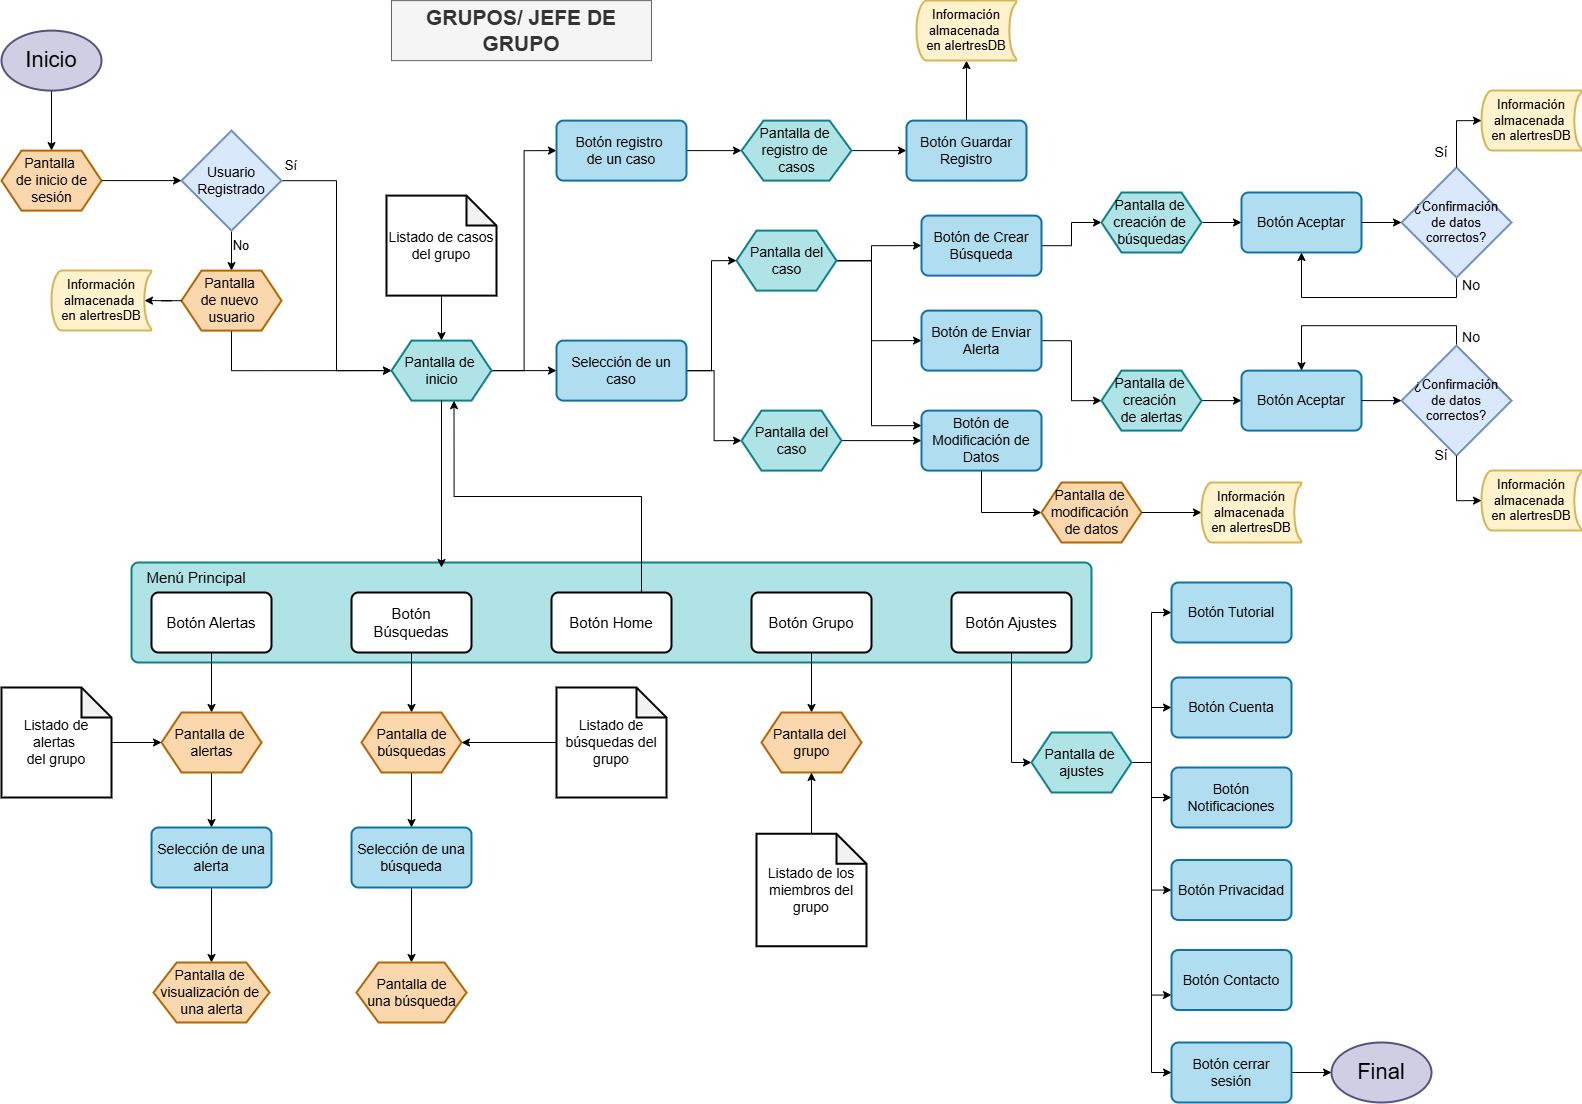
\includegraphics[width=1.3\linewidth, angle=270, keepaspectratio]{img/DiagramaFlujoGrupos.png}
        \caption{Diagrama navegacional del prototipo creado para el perfil de grupos o jefes de grupos. \textit{Fuente propia.}}
        \label{DFlujo_Grupos}
    \end{figure}
    
\clearpage
\vspace{15cm}

    \figura{1}{img/DiagramaFlujoMiembros.png}{Diagrama navegacional del prototipo creado para el perfil de miembros. \textit{Fuente propia.}}{DFlujo_Miembros}{keepaspectratio}
    
\vspace{30cm}



%%%%%%%%%%%%%%%%%%%%%%%%%%%%% PANTALLAS DEL PROTOTIPO %%%%%%%%%%%%%%%%%%%%%%%%%%%%%
    \subsection{Pantallas principales del prototipo implementado}
     
     Como se ha mencionado previamente, inicialmente se desarrolló un primer prototipo que utilizaba la misma interfaz para todos los tres tipos usuarios, lo que hacía que ciertas funcionalidades estuviesen visibles pero a su vez bloquedas en función del tipo de usuario, algo que tras reflexionar se consideró como poco funcional lo que llevó a la realización del segundo prototipo y final. Algunas de las pantallas de ese primer prototipo se recogen en la figura \ref{capturasAlertResV1}. Teniendo en cuenta esto, en este apartado se presentan las princpales pantallas y funcionalidades del último prototipo final implementado. 

     \figura{1}{img/Resultados/PantallasPrototipo1.png}{Algunas pantallas del primer prototipo. \textit{Fuente propia.}}{capturasAlertResV1}{keepaspectratio}

     El prototipo final recoge tres interfaces diferentes para cada tipo de usuario, consiguiendo una mejor visualización y usabilidad por parte de los usuarios. Estas interfaces están unidas por una misma pantalla a modo de inicio de sesión, donde se selecciona el usuario con el que se desea acceder. En las figuras \ref{capAlertResV2_Grupos}--\ref{capAlertResV2_Miembros} se encuentran recogidas todas las pantallas principales para cada tipo de usuario.
     
     \figura{1}{img/Resultados/DiagramaPantallasGrupo.png}{Resumen de las pantallas del segundo prototipo implementado para un usuario con rol de grupo. \textit{Fuente propia.}}{capAlertResV2_Grupos}{keepaspectratio}
     
     \figura{1}{img/Resultados/DiagramaPantallasVoluntario.png}{Resumen de las pantallas del segundo prototipo implementado para un usuario con rol de voluntario. \textit{Fuente propia.}}{capAlertResV2_Voluntarios}{keepaspectratio}

     \figura{1}{img/Resultados/DiagramaPantallasMiembro.png}{Resumen de las pantallas del segundo prototipo implementado para un usuario con rol de miembro de un grupo. \textit{Fuente propia.}}{capAlertResV2_Miembros}{keepaspectratio}


\clearpage
     \subsubsection{Pantalla de inicio de sesión}
     Es la primera pantalla que se mostrará tras abrir el prototipo. Esta pantalla es auxiliar y su objetivo es simular una pantalla de inicio de sesión.

     Tiene distintos componentes relevantes:
     \begin{itemize}
         \item Imagen del logo de AlertRes.
         \item Desplegable de selección de usuario entre aquellos registrados en la tabla \texttt{users} de la base de datos.
         \item Botón `Entrar con usuario seleccionado' para acceder a la pantalla de inicio correspondiente al usuario seleccionado en el desplegable.
         \item Botón `Crear nuevo usuario' para registrar a un nuevo usuario de la aplicación.
         
     \end{itemize}

     \figura{0.35}{img/Resultados/Captura_AlertRes_inicioSesion.jpg}{Pantalla de inicio de sesión. \textit{Fuente propia.}}{app_inicioSesion}{keepaspectratio}



     \subsubsection{Pantalla de registro de un nuevo usuario}

     Esta pantalla es accesible a través del botón que se encuentra en la pantalla de inicio de sesión: `Crear nuevo usario'. 
     
     La pantalla cuenta con distintos campos que debe rellenar el interesado para crear un nuevo usuario (nombre, apellidos, DNI, teléfono, email...). Además, se muestra un desplegable donde el usuario debe seleccionar su rol entre `Voluntario'~ o `Grupo'~\footnote{Los miembros de un grupo deben realizar un primer registro como usuarios voluntarios y luego el jefe de grupo desde un usario `Grupo'~ dará de alta al miembro desde la pantalla de información del grupo y se cambiará automáticamente el rol de `Voluntario'~ a `Miembro'~ de un grupo}. En caso de seleccionar el rol de usuario `Grupo', se desplegarán automáticamente otros campos rellenables donde introducir la información del grupo.

     En el backend esta información se recoge en las tablas \texttt{people} y \texttt{users}.

     \figura{0.35}{img/Resultados/Captura_AlertRes_registroUsuario.jpg}{Pantalla de registro de un nuevo usuario. \textit{Fuente propia.}}{app_registroUsuario}{keepaspectratio}



     \subsubsection{Pantalla de casos del grupo}
     Esta pantalla es la pantalla de inicio de los usuarios con rol de `Grupo'~ y únicamente está disponible para esos usuarios.

     La pantalla recoge todos los casos del grupo tanto los que se encuentran actualmente activos como los que no. En cada caso se muestra información básica del incidente y una etiqueta que muestra si el caso está actualmente activo o no. Asimismo, se puede seleccionar el caso para acceder a su información en la pantalla del caso.

     Además, esta pantalla cuenta con otros elementos como:
     \begin{itemize}
     \item Un campo identificativo donde se muestra el nombre del grupo y del jefe regristrado.
     \item Botón `Registrar caso'~desde donde se podrá acceder a una nueva pantalla donde registrar un caso nuevo.
     \end{itemize}

     En la parte inferior se encuentra el menú principal que llevará al resto de pantallas (pantalla de información del grupo, de búsquedas, de alertas y de ajustes) a las que tiene acceso el usuario que ha iniciado sesión con rol de grupo.

     \figura{0.35}{img/Resultados/Captura_AlertRes_casosGrupo.jpg}{Pantalla de casos del grupo logueado. \textit{Fuente propia.}}{app_casosGrupo}{keepaspectratio}




     \subsubsection{Pantalla de registro de casos}
     A esta pantalla se accede desde el botón de la pantalla anterior y contiene una serie de campos rellenables donde se recopila toda la información del incidente, de la persona desaparecida y del propio denunciante. Estos campos incluyen todos los atributos que se incluirán en las tablas \texttt{missing people}, \texttt{cases}, \texttt{people} y \texttt{reporters} de la base de datos. La inclusión en la base de datos no se realizará hasta presionar el botón de `Guardar'.

     En la parte inferior se encuentra el menú principal que llevará al resto de pantallas a las que tiene acceso el usuario que ha iniciado sesión con rol de grupo.

     \figura{0.33}{img/Resultados/Captura_AlertRes_nuevoCaso.jpg}{Pantalla de creación de un nuevo caso. \textit{Fuente propia.}}{app_nuevoCaso}{keepaspectratio}


     

     \subsubsection{Pantalla de información de un caso}
     Esta pantalla está únicamente disponible para grupos y recoge toda la información disponible en la base de datos relativa al incidente y a la persona desaparecida del caso que se haya seleccionado. Además, cuenta con cuatro botones principales:
     \begin{itemize}
         \item Botón de modificación de los datos, en caso de que sea necesario modificar algún campo erróneo del caso. Este botón se encuentra disponible tanto para casos cuyo expediente se encuentra en activo como para los cerrados.
         \item Botón de creación de una alerta que llevará a la pantalla correspondiente para la emisión de una alerta sobre el caso. Únicamente está disponible para los casos que se encuentran actualmente activos.
         \item Botón de creación de una búsqueda que llevará al a pantalla correspondiente, en caso de que fuese necesario organizar una búsqueda sobre el terreno. Únicamente se encuentra disponible para los casos que se enucentran actualmente activos.
         \item Botón de cierre del caso, que únicamente está disponible para casos abiertos y que lleva a la pantalla de cierre del caso desde donde se podrá cambiar el estado del caso y rellenar la información post-intervención.
     \end{itemize}
     
     En la parte inferior se encuentra el menú principal que llevará al resto de pantallas a las que tiene acceso el usuario que ha iniciado sesión con rol de grupo.

     %\figura{0.35}{img/Resultados/Captura_AlertRes_infoCaso.png}{Pantalla de información de un caso. \textit{Fuente propia.}}{app_infoCaso1}{keepaspectratio}

     %\figura{0.35}{img/Resultados/Web_AlertaEnviada.png}{Pantalla de información de un caso con sus botones. \textit{Fuente propia.}}{app_infoCaso2}{keepaspectratio}

     \begin{figure}
        \centering
        % Primera imagen
        \begin{subfigure}{0.35\textwidth}
            \centering
            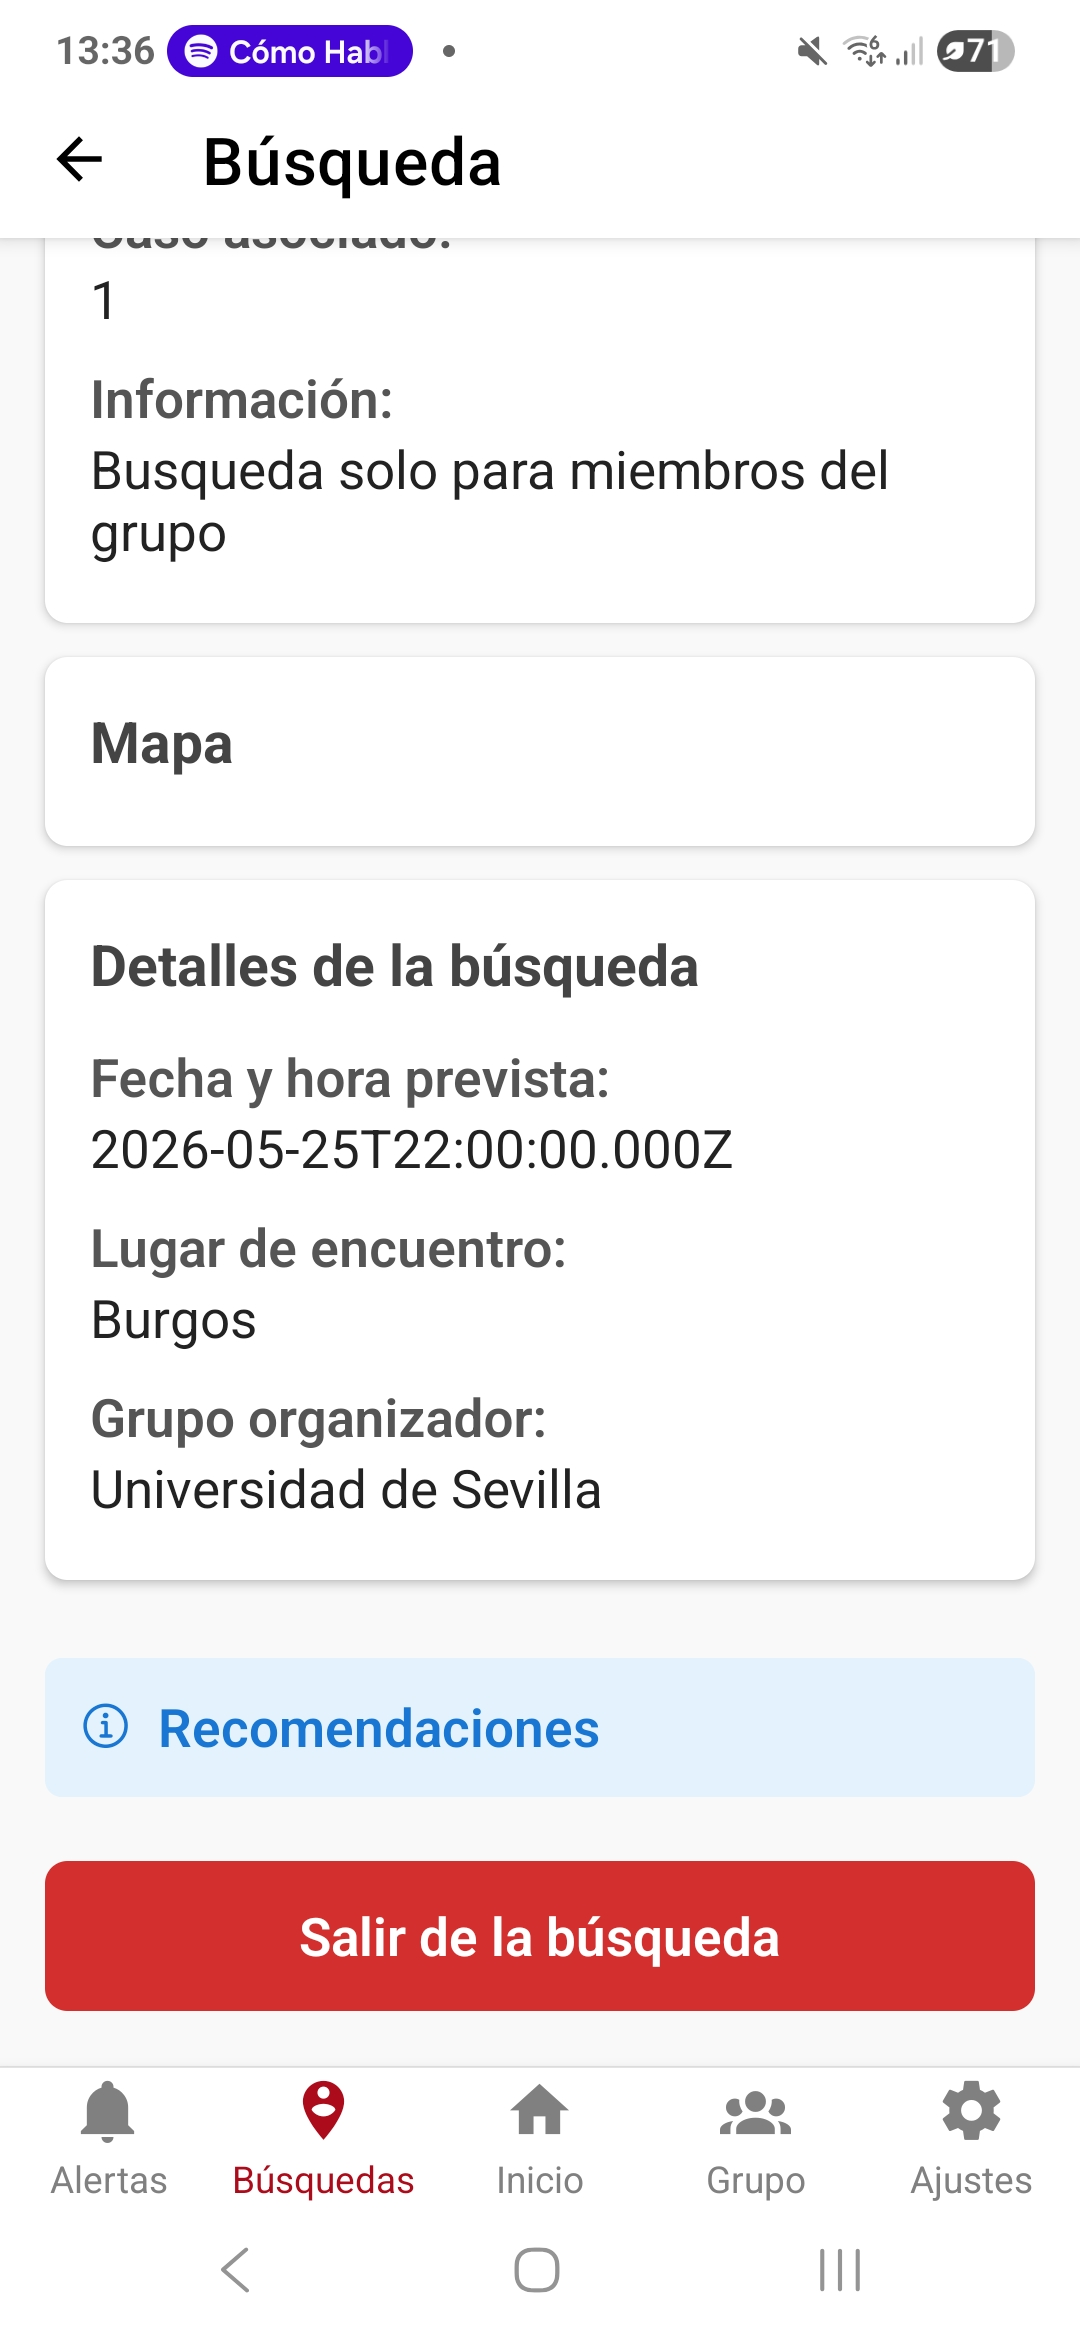
\includegraphics[width=\linewidth]{img/Resultados/Captura_AlertRes_infoCaso.jpg}
        \end{subfigure}
        \hfill
        % Segunda imagen
        \begin{subfigure}{0.35\textwidth}
            \centering
            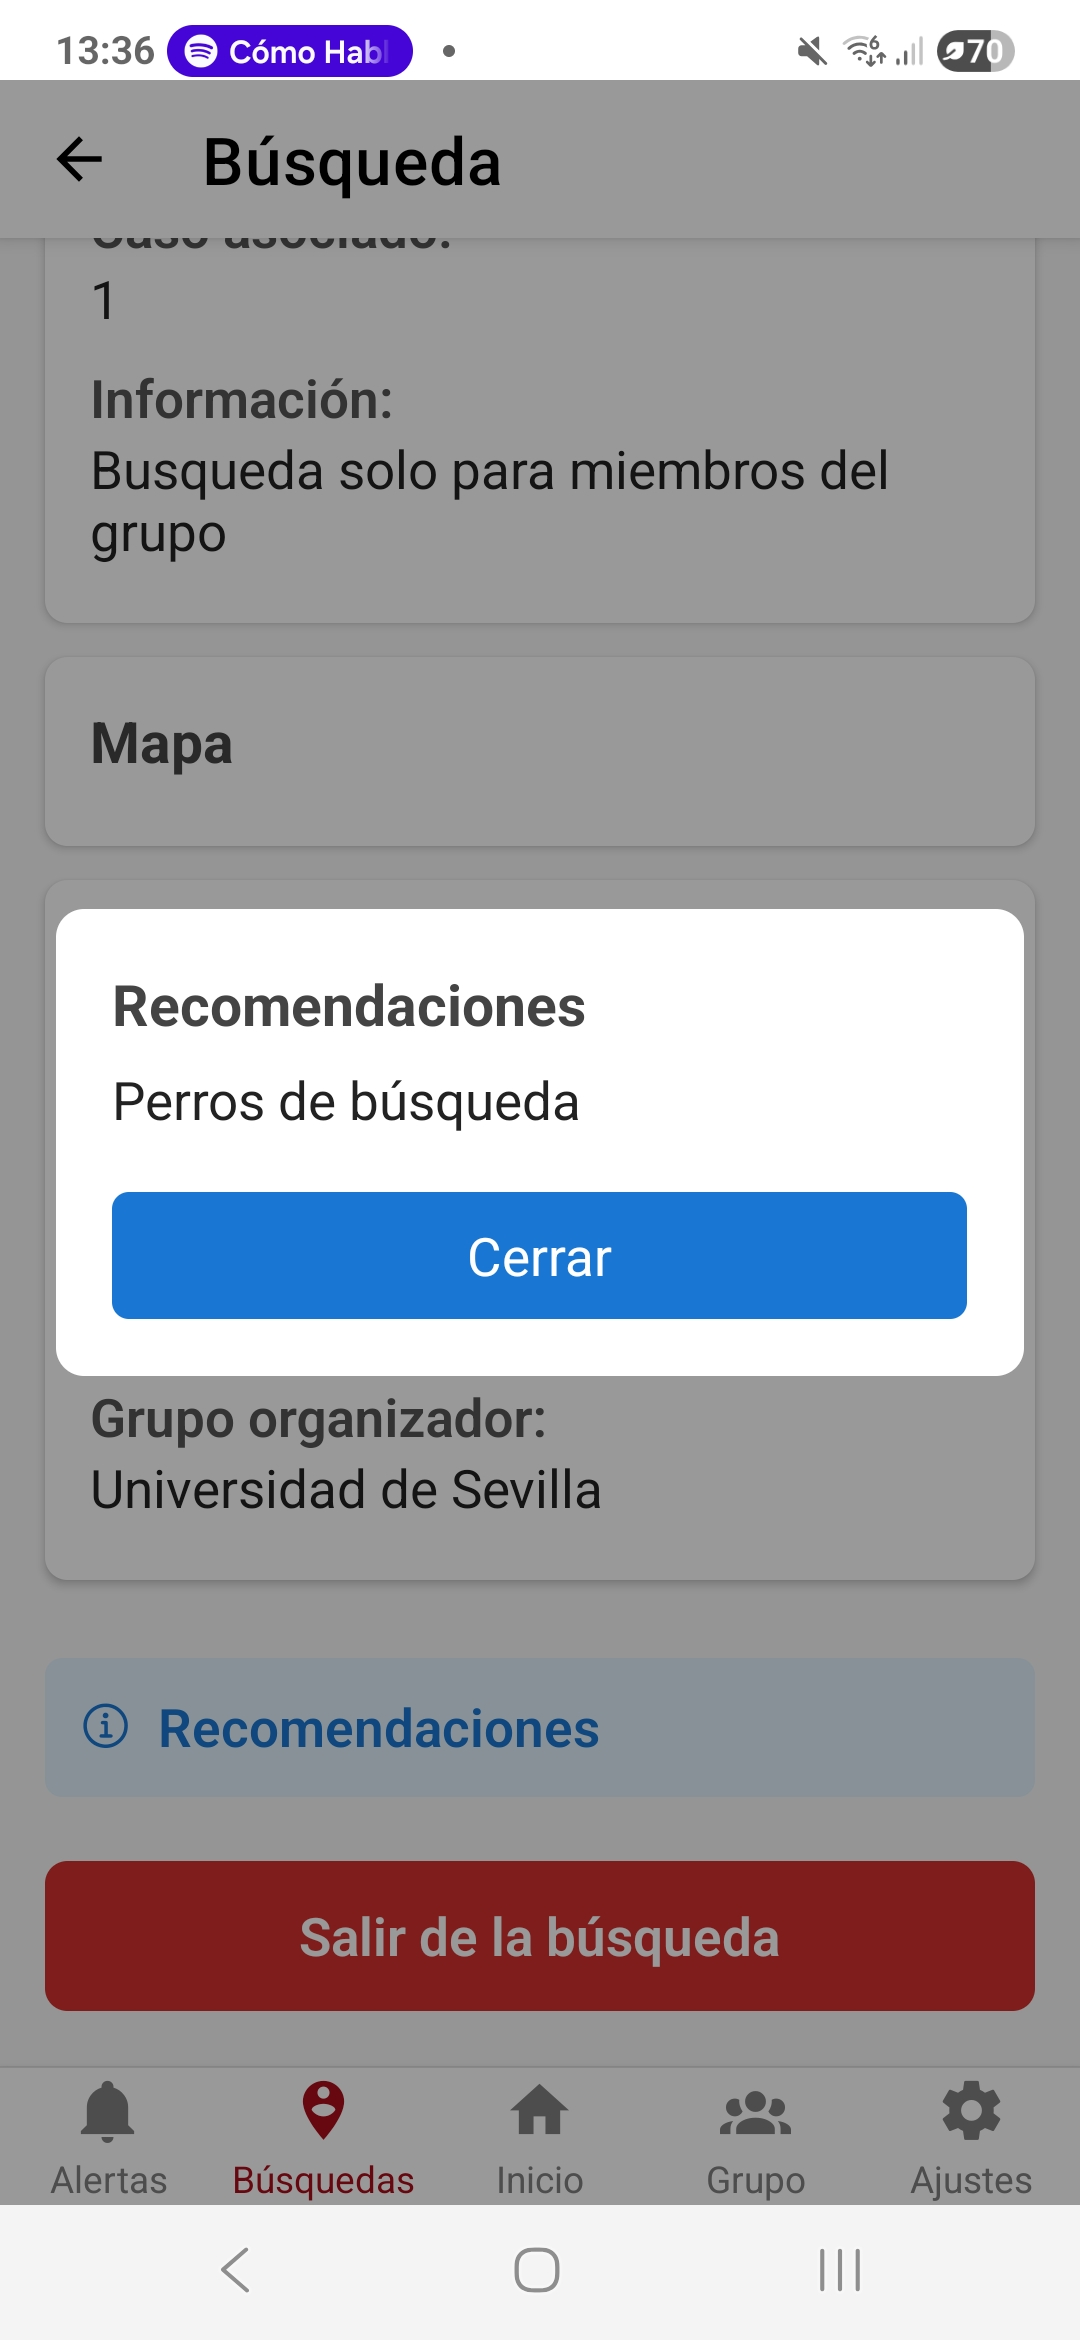
\includegraphics[width=\linewidth]{img/Resultados/Captura_AlertRes_infoCaso2.jpg}
        \end{subfigure}
        \hfill
        % Tercera imagen
        \begin{subfigure}{0.35\textwidth}
            \centering
            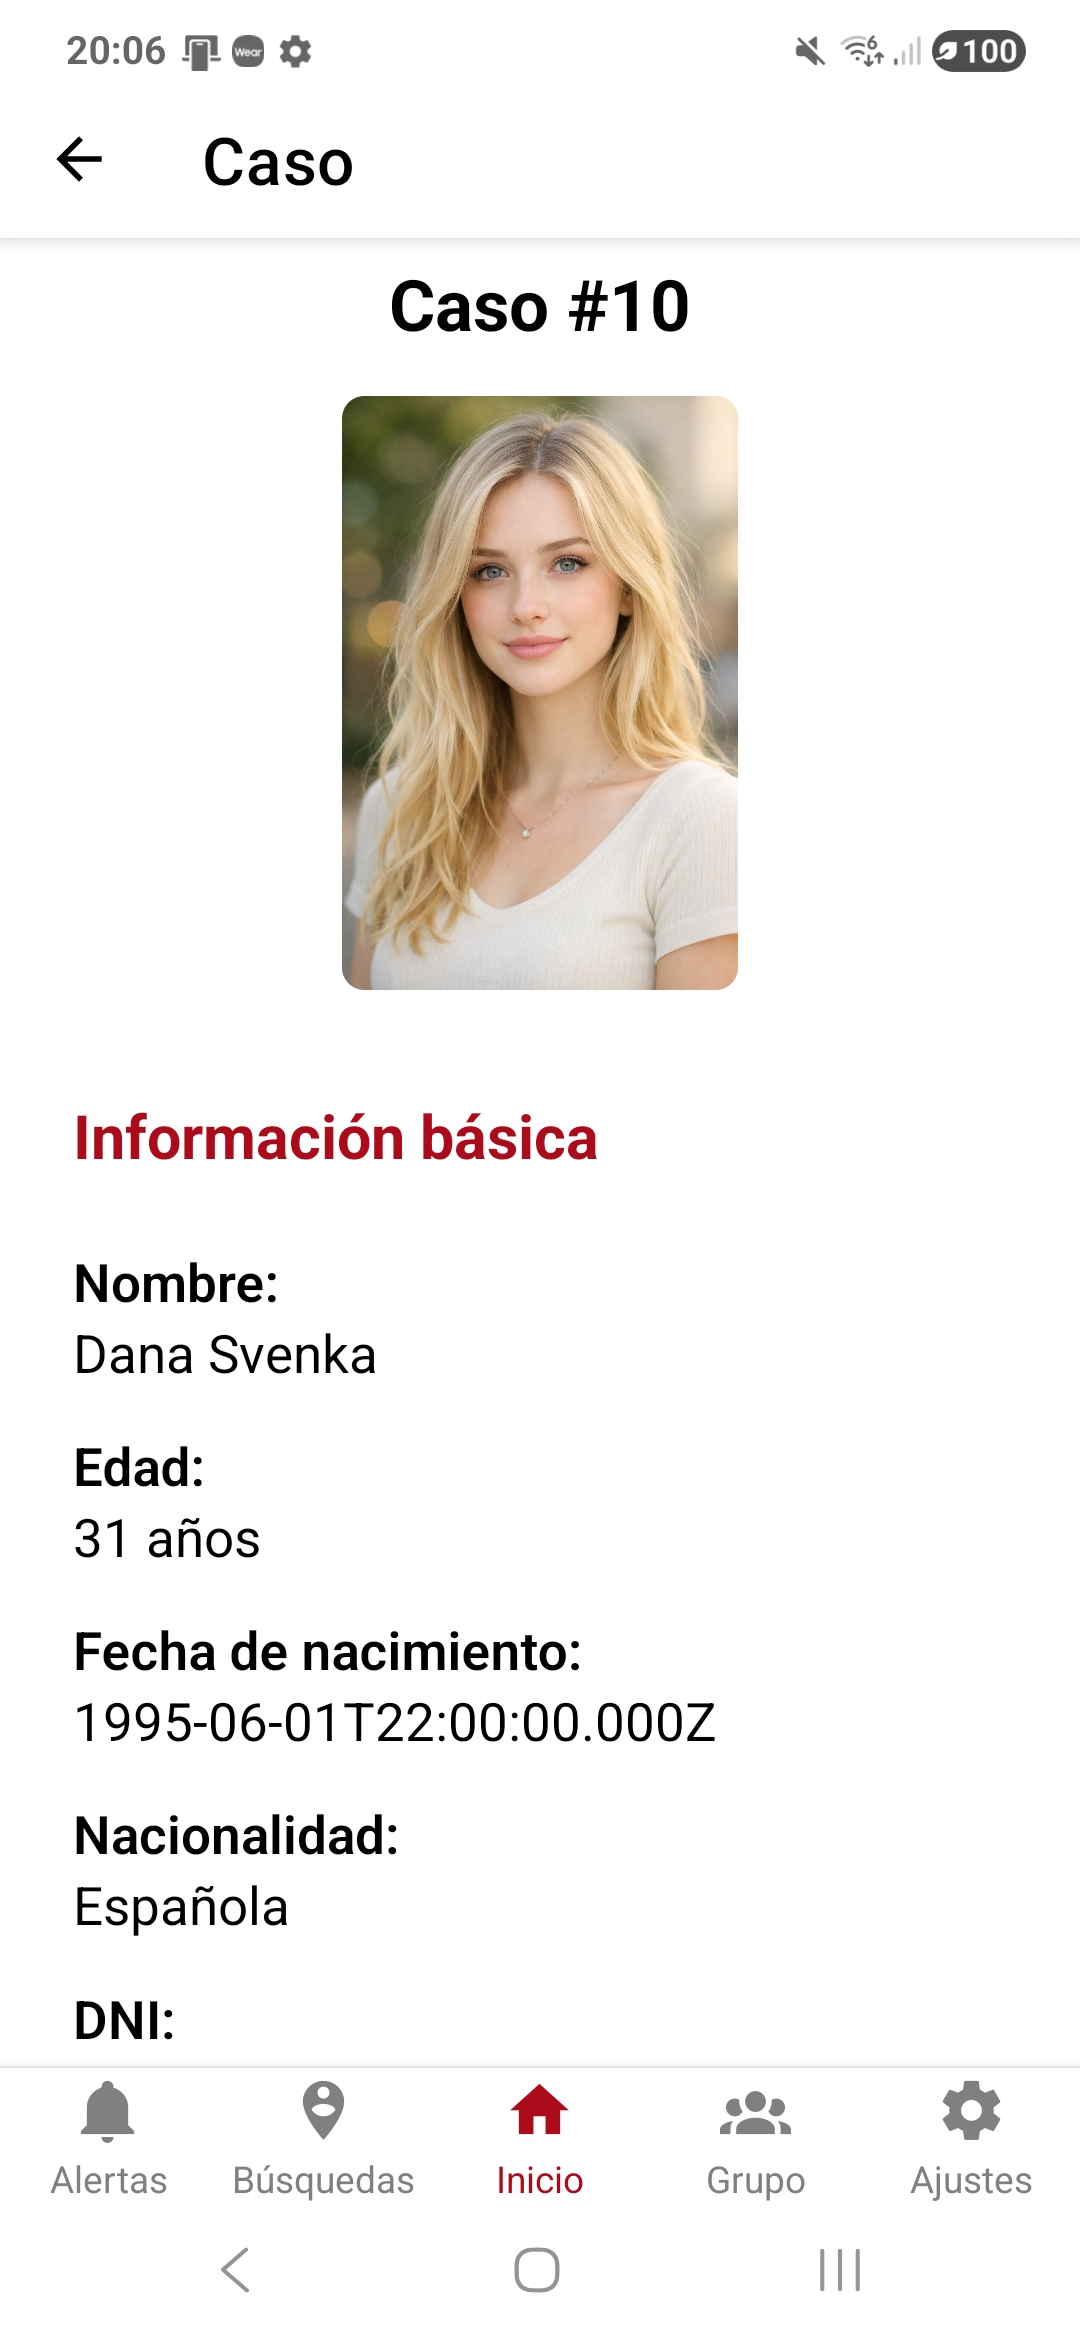
\includegraphics[width=\linewidth]{img/Resultados/Captura_AlertRes_infoCaso3.jpg}
        \end{subfigure}
        \hfill
        % Cuarta imagen
        \begin{subfigure}{0.35\textwidth}
            \centering
            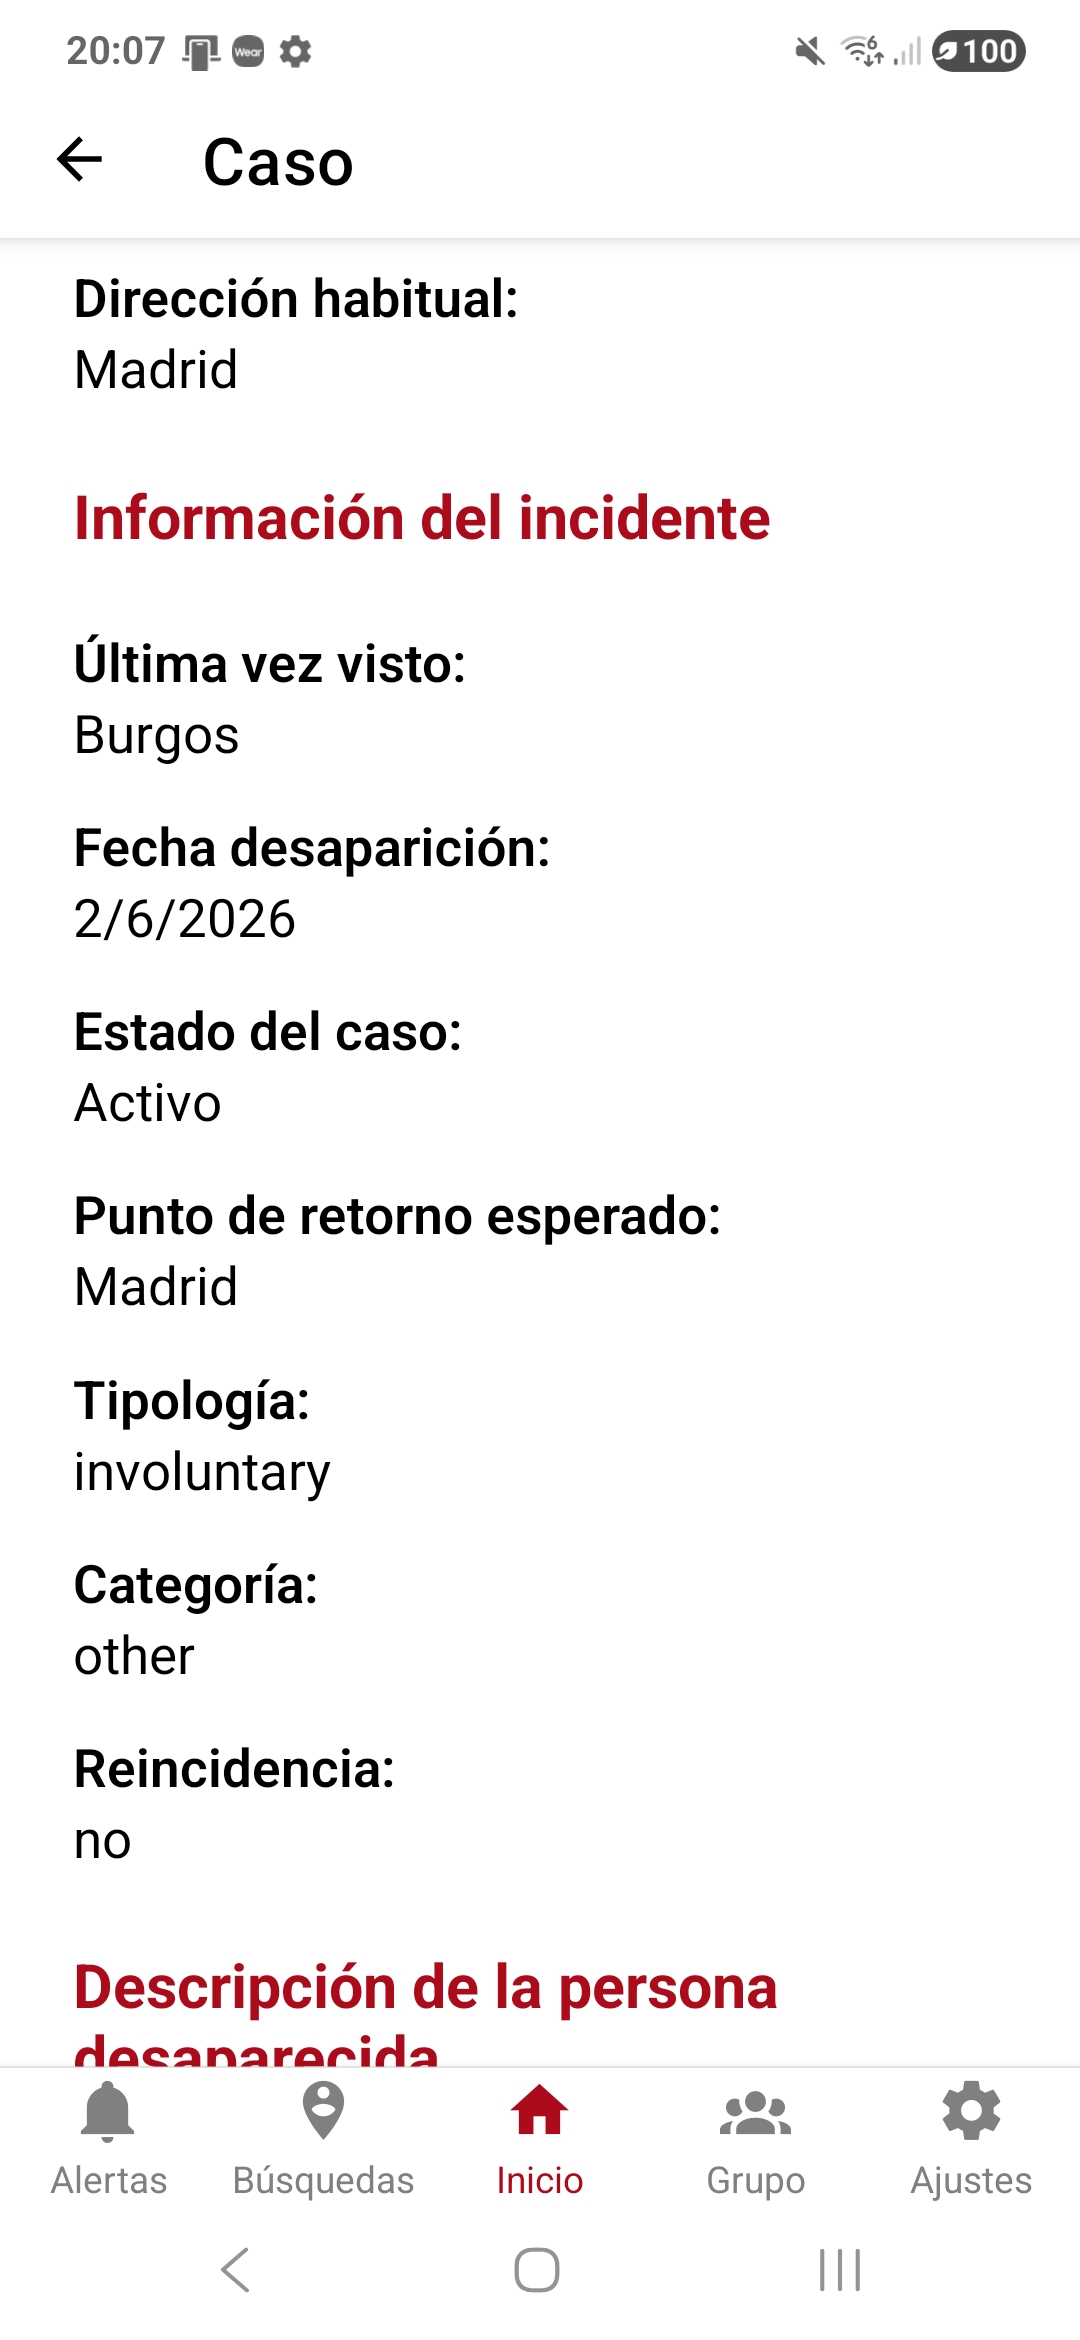
\includegraphics[width=\linewidth]{img/Resultados/Captura_AlertRes_infoCaso4.jpg}
        \end{subfigure}
        \hfill
        \caption{Pantalla de información de un caso con sus botones. \textit{Fuente propia.}}
        \label{app_infoCaso}
    \end{figure}

    \clearpage

     \subsubsection{Pantalla de creación de búsquedas}
     La pantalla de creación de búsquedas se utiliza para lo que su nombre indica y es accesible desde la pantalla que recoge la información de un caso que se encuentra activo. Desde aquí se recoge la información complementaria para la creación de la búsqueda, como el lugar y la fecha de encuentro o las recomendaciones para los participantes en la búsqueda. Esta información luego se añade a la base de datos en la tabla \texttt{searches}.

     En la parte inferior se encuentra el menú principal que llevará al resto de pantallas a las que tiene acceso el usuario que ha iniciado sesión con rol de grupo.


    \begin{figure}[h!]
        \centering
        % Primera imagen
        \begin{subfigure}{0.35\textwidth}
            \centering
            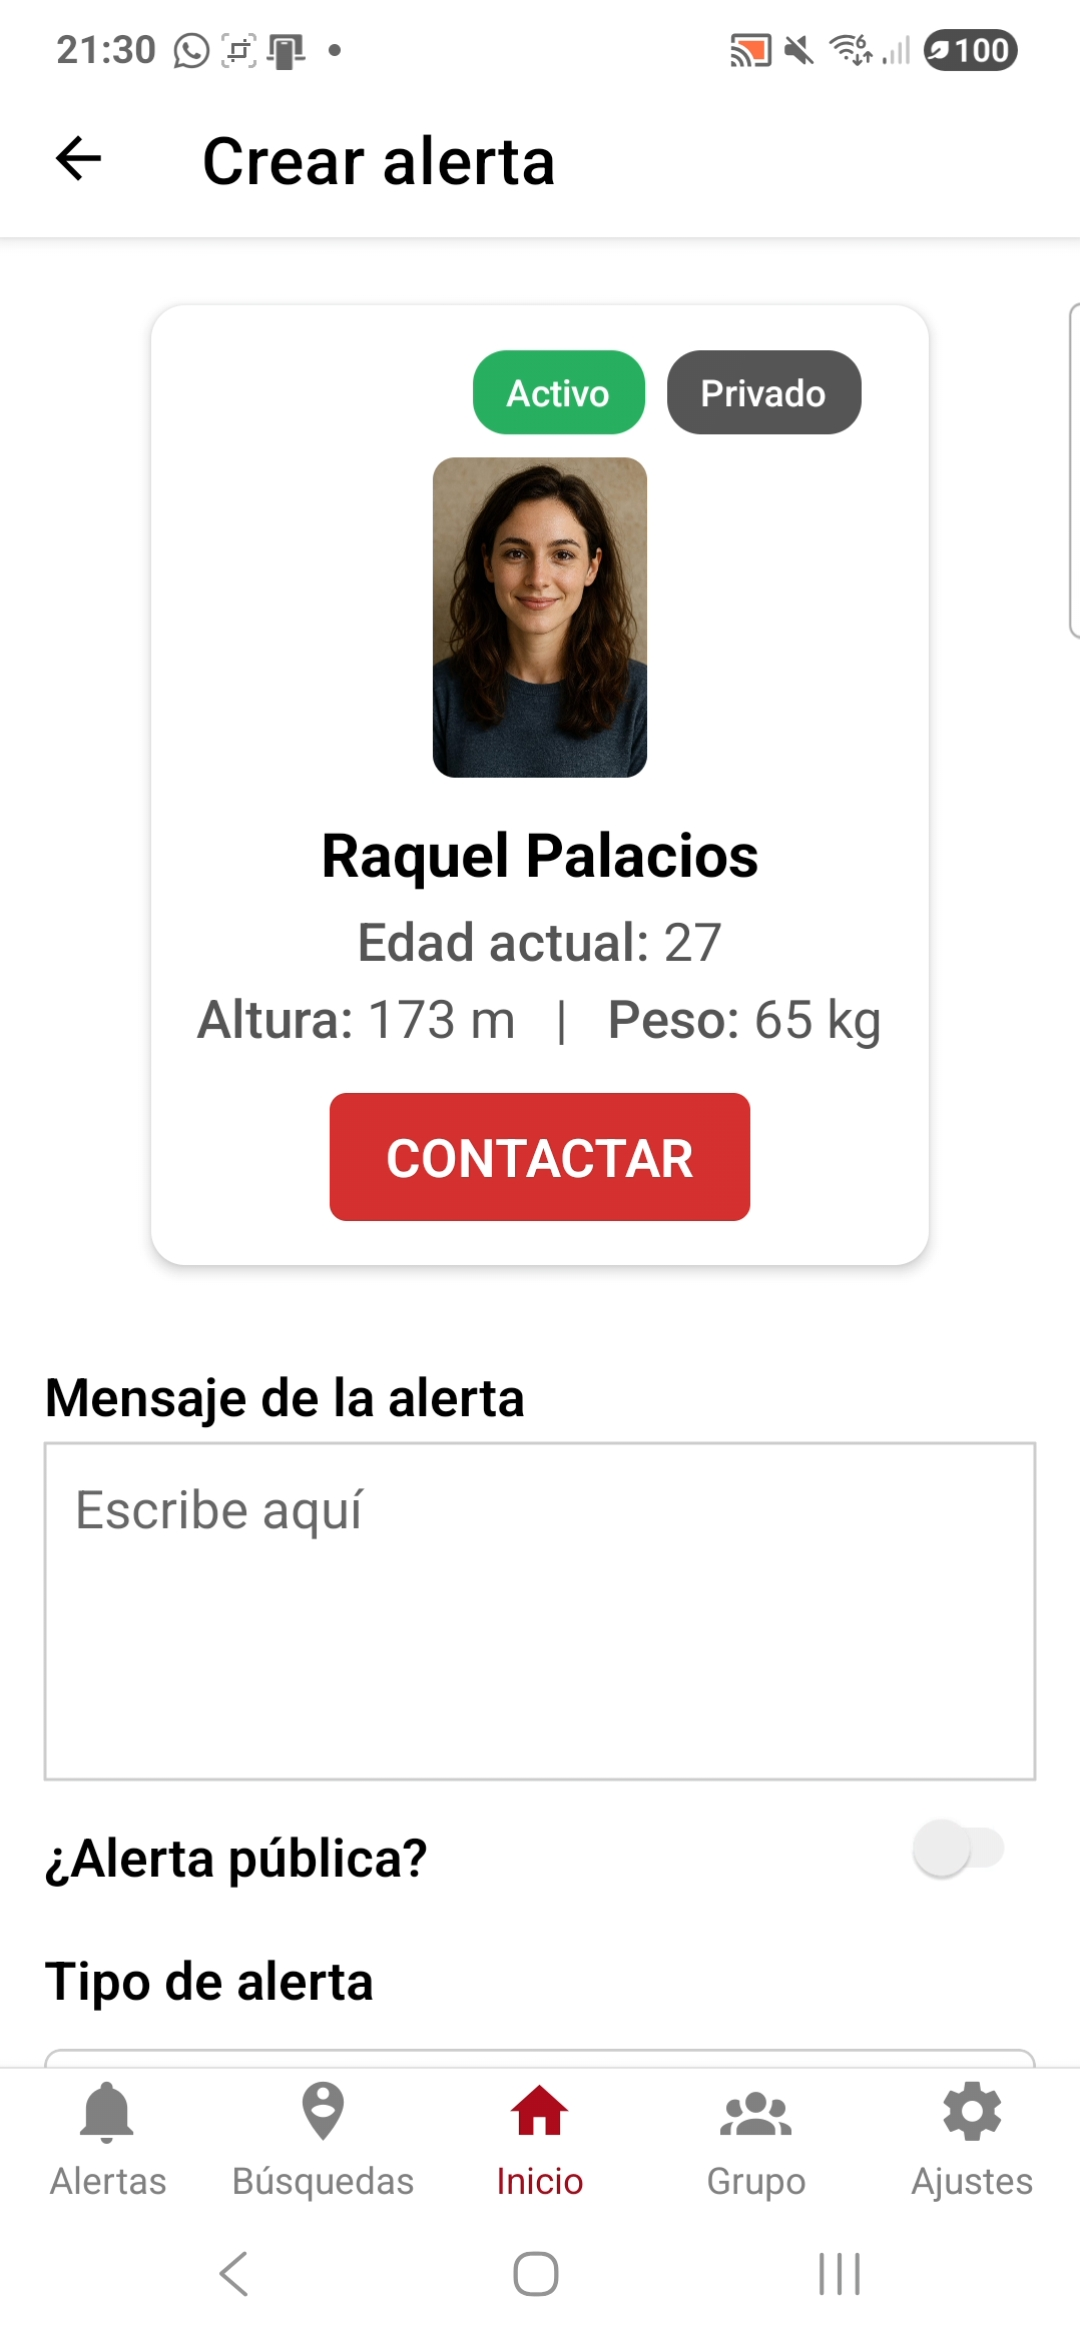
\includegraphics[width=\linewidth]{img/Resultados/Captura_AlertRes_nuevaBusqueda.jpg}
        \end{subfigure}
        \hfill
        % Segunda imagen
        \begin{subfigure}{0.35\textwidth}
            \centering
            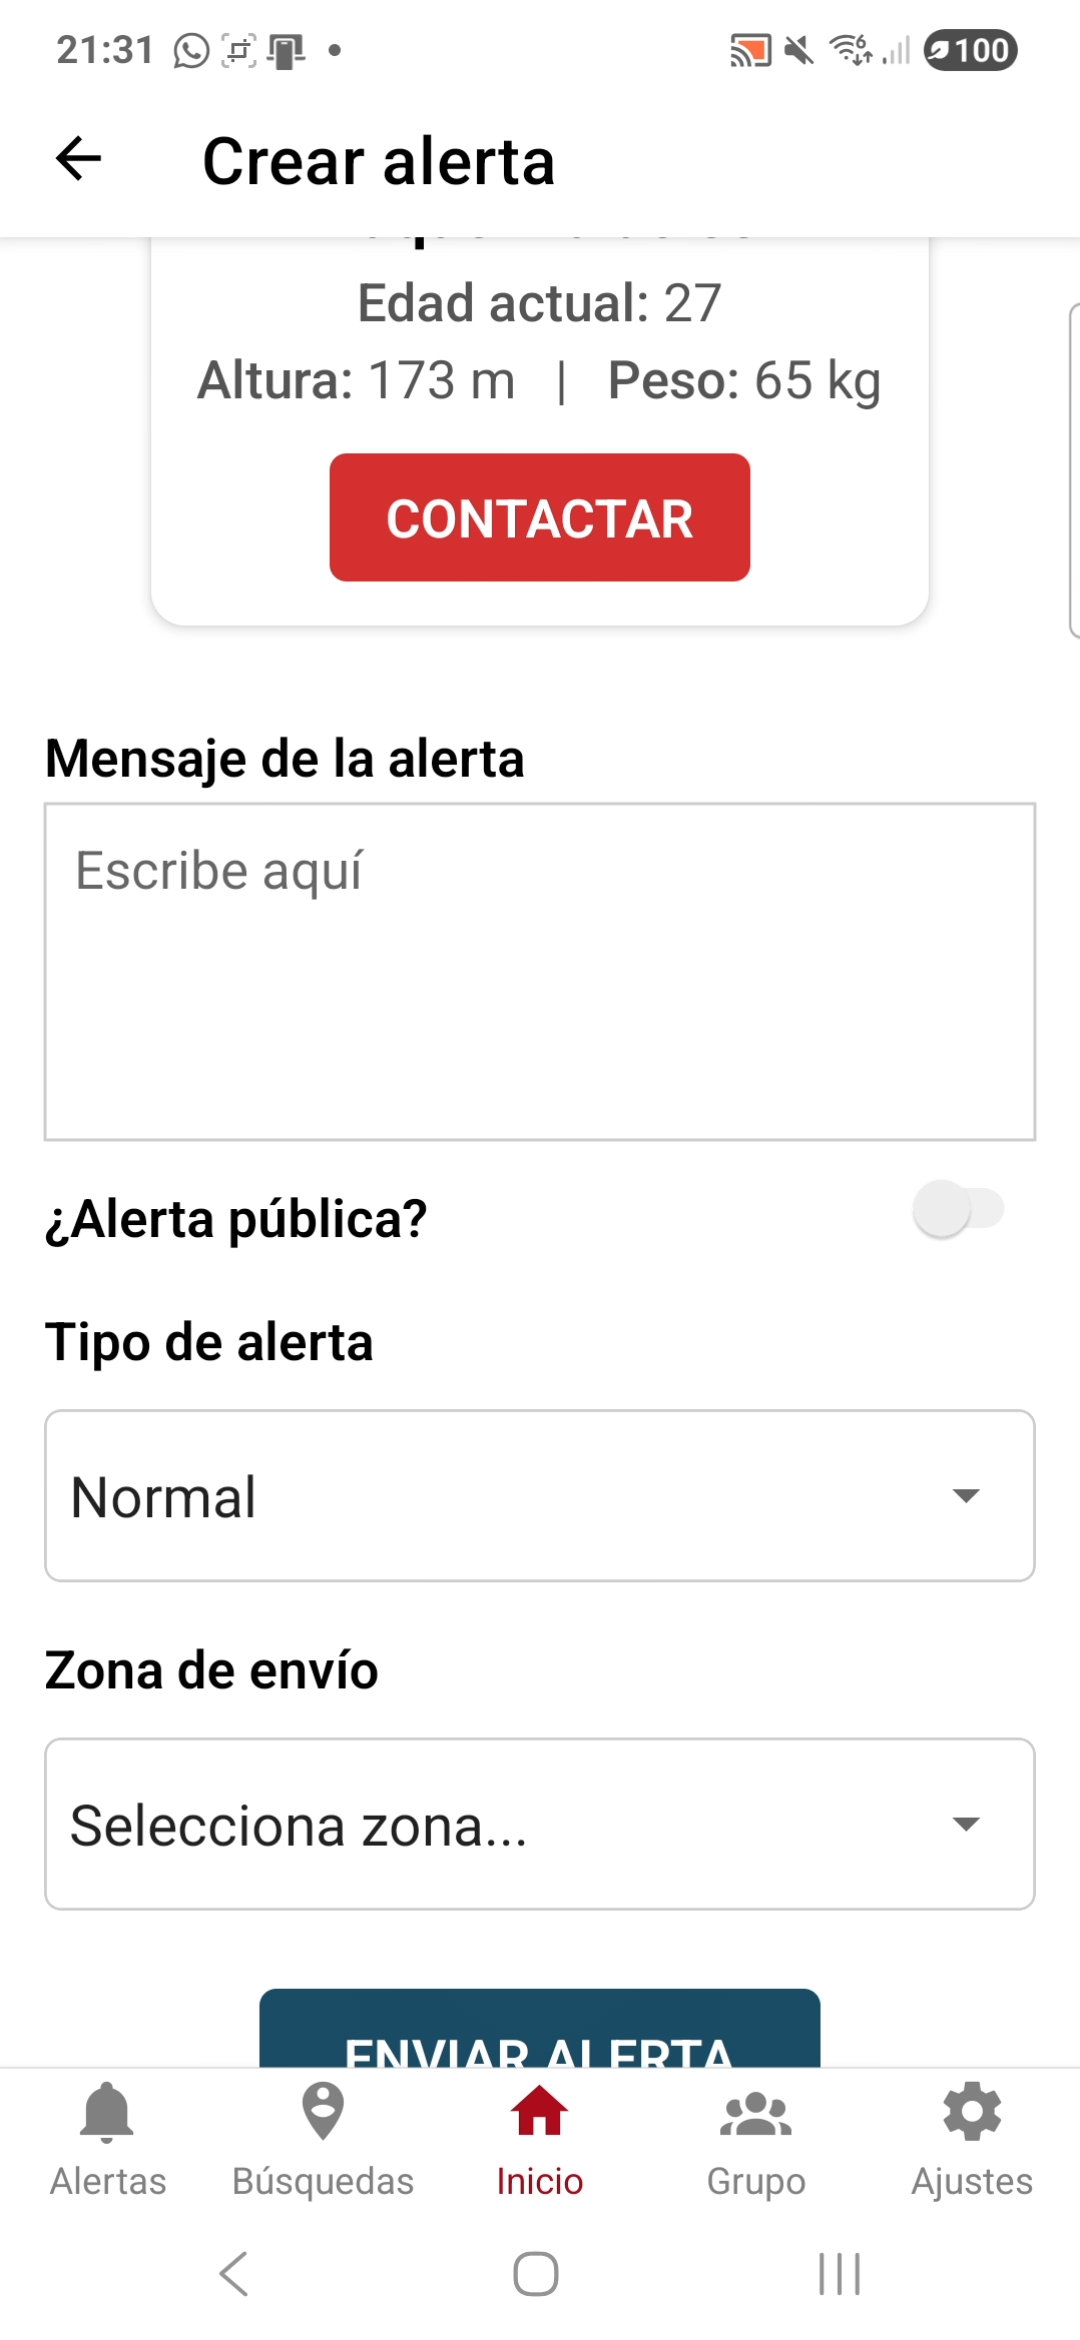
\includegraphics[width=\linewidth]{img/Resultados/Captura_AlertRes_nuevaBusqueda2.jpg}
        \end{subfigure}
        \caption{Pantalla de creación de búsquedas. \textit{Fuente propia.}}
        \label{app_nuevaBusqueda}
    \end{figure}

     %\figura{0.35}{img/Resultados/Web_AlertaEnviada.png}{Pantalla de creación de búsquedas. \textit{Fuente propia.}}{app_nuevaBusqueda}{keepaspectratio}


     \subsubsection{Pantalla de creación de alertas}
     La pantalla de creación de alertas, al igual que la de creación de búsquedas, solo es accesible desde la pantalla de información de un caso que se encuentra activa. Esta pantalla recoge los campos complementarios necesarios para lanzar una alerta sobre el caso a la población, lo que se considera alerta pública, o a los propios miembros del grupo, que se considera alerta privada. Algunos de los campos a completar son el tipo de alerta, un mensaje o la zona de envío de la misma. Esta información se recogerá en la tabla \texttt{alerts} de la base de datos.
     
\vspace{1cm}

     En la parte inferior se encuentra el menú principal que llevará al resto de pantallas a las que tiene acceso el usuario que ha iniciado sesión con rol de grupo.

     \begin{figure}[h!]
        \centering
        % Primera imagen
        \begin{subfigure}{0.35\textwidth}
            \centering
            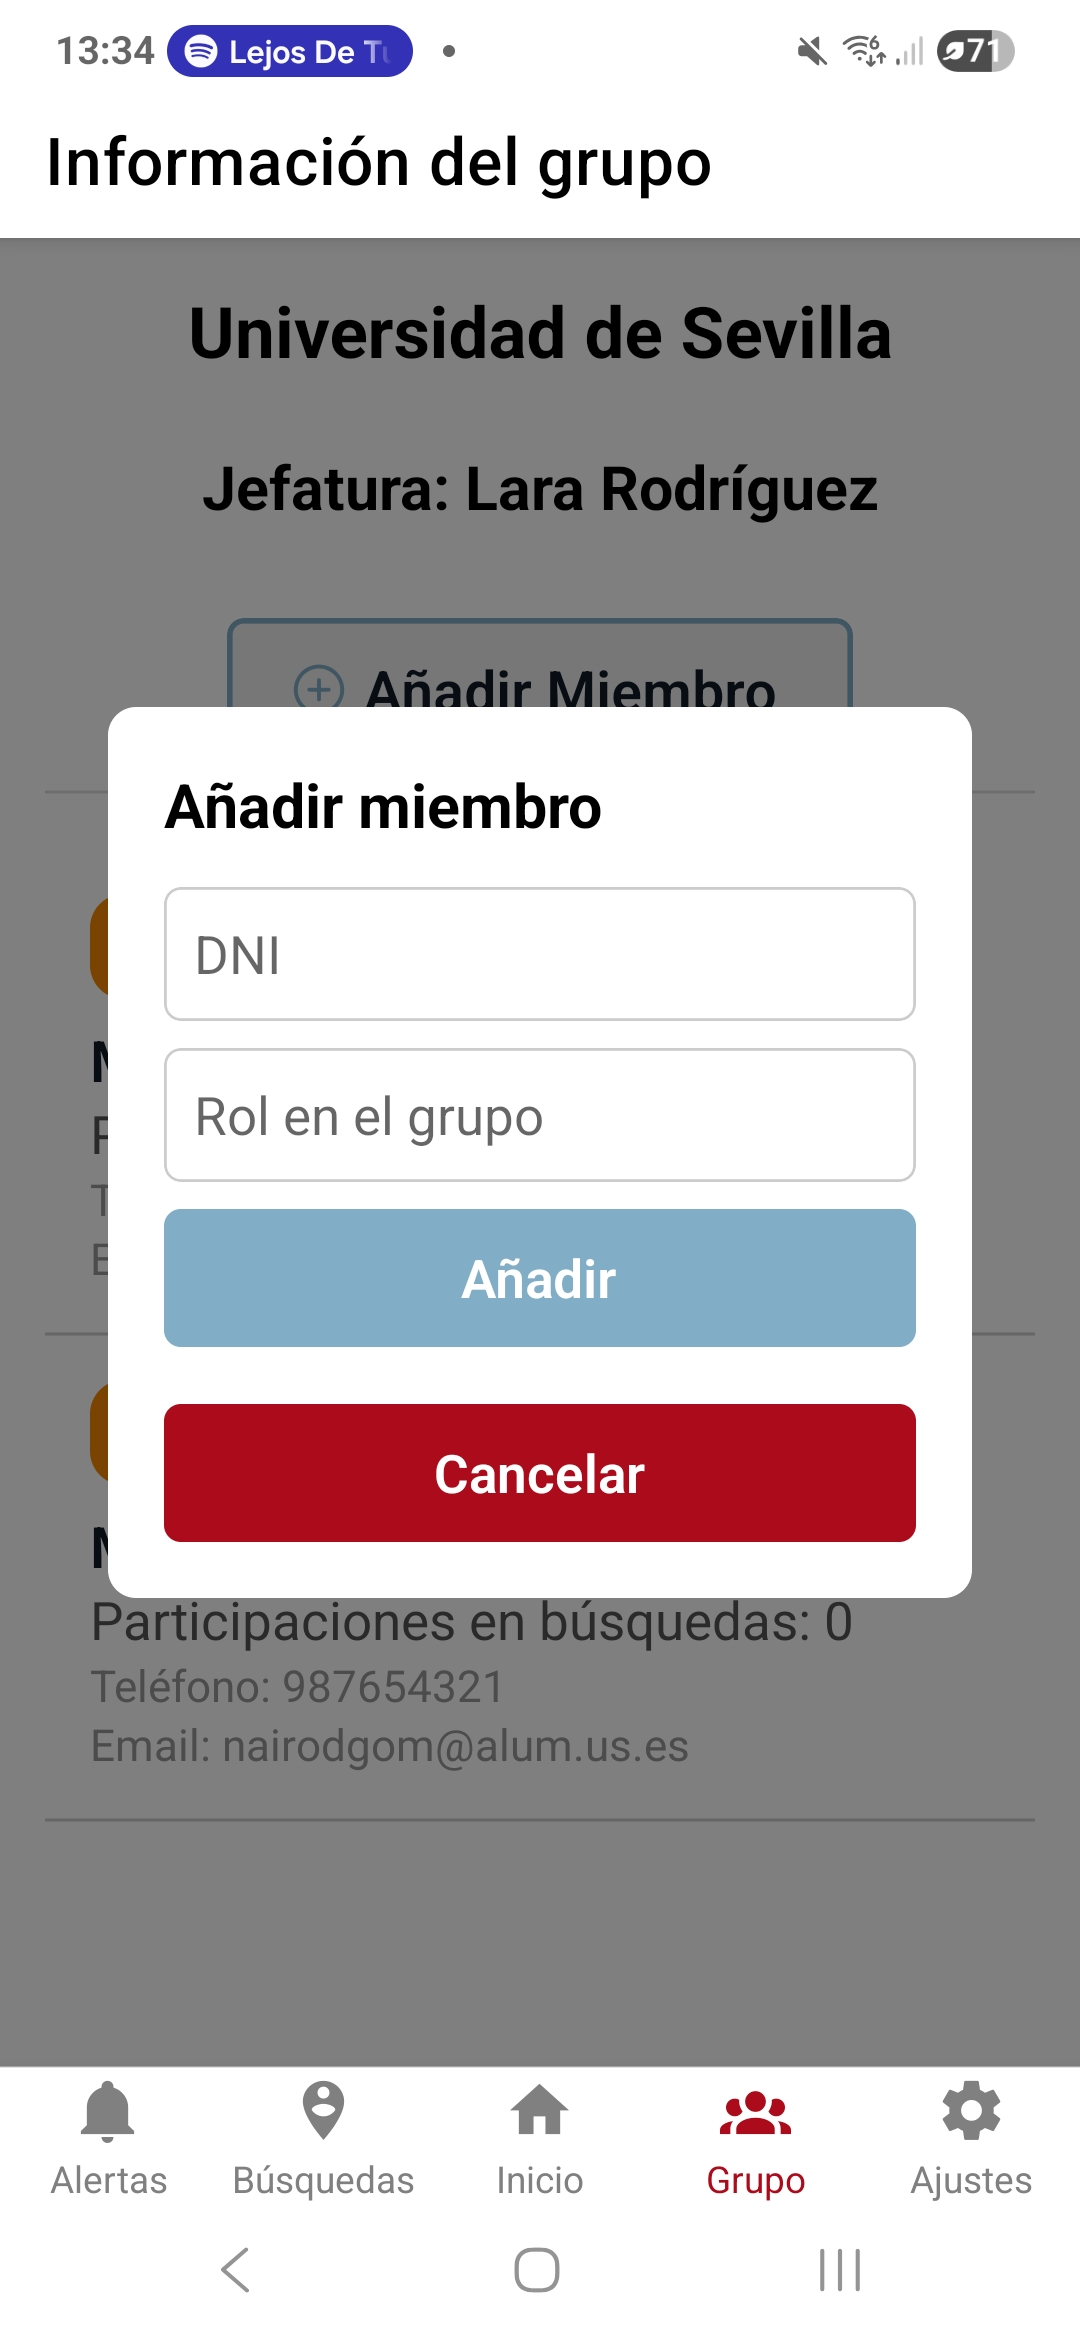
\includegraphics[width=\linewidth]{img/Resultados/Captura_AlertRes_nuevaAlerta.jpg}
        \end{subfigure}
        \hfill
        % Segunda imagen
        \begin{subfigure}{0.35\textwidth}
            \centering
            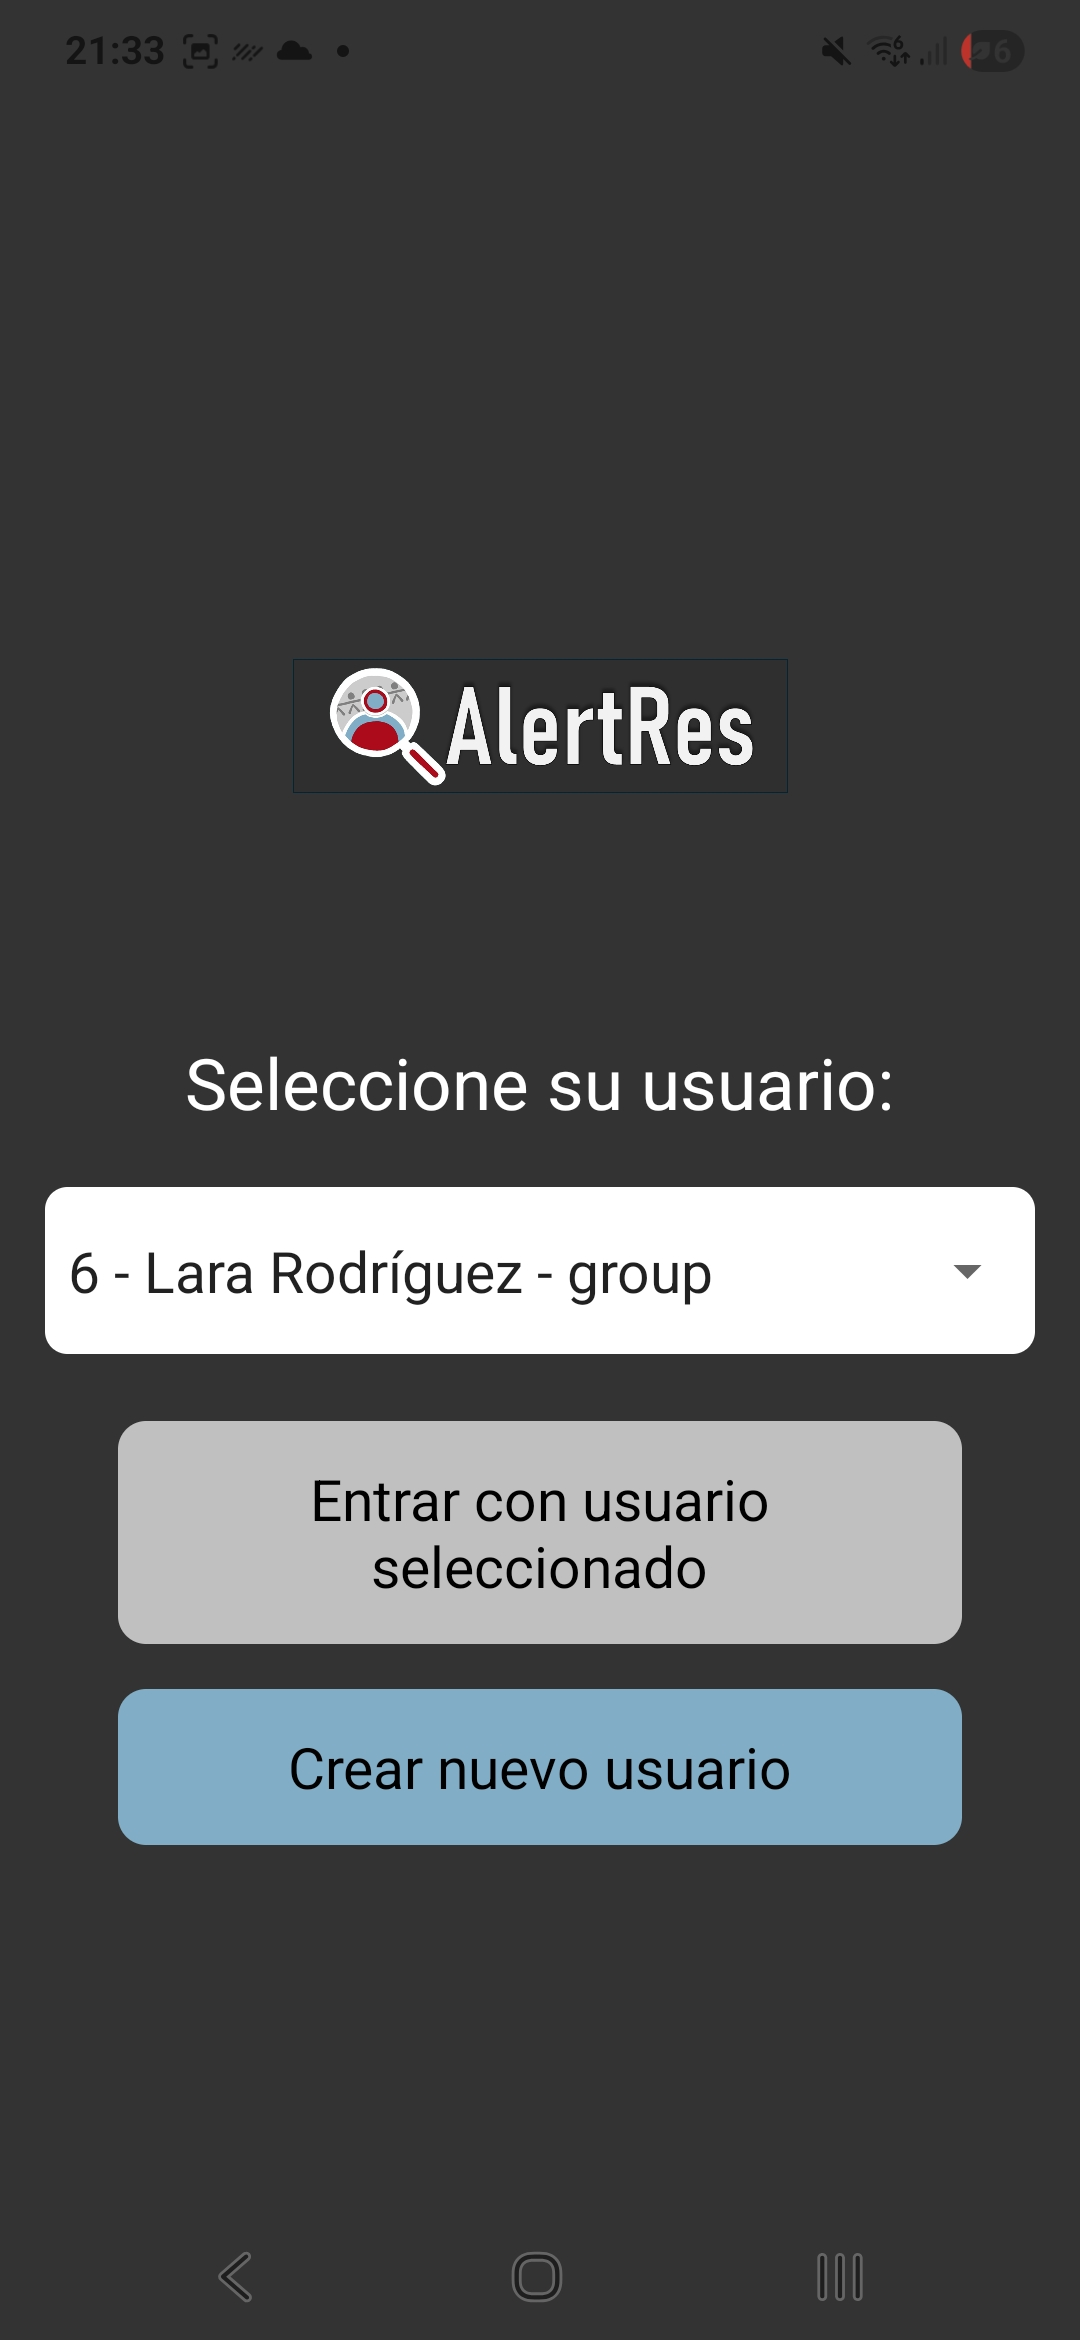
\includegraphics[width=\linewidth]{img/Resultados/Captura_AlertRes_nuevaAlerta2.jpg}
        \end{subfigure}
        \caption{Pantalla de creación de alertas. \textit{Fuente propia.}}
        \label{app_nuevaAlerta}
    \end{figure}

     %\figura{0.35}{img/Resultados/Web_AlertaEnviada.png}{Pantalla de creación de una alerta. \textit{Fuente propia.}}{app_nuevaAlerta}{keepaspectratio}

    \subsubsection{Pantalla de alertas}
    Esta pantalla es la pantalla Home de los usuarios con rol de `Miembros'~ y de `Voluntarios'. Mientras que los usuarios con rol `Grupo'~ tendrán acceso a esta pantalla desde el apartado de `Alertas'~ del menú inferior.
    
    En esta pantalla se puede ver la lista de desaparecidos de los cuales se han lanzado alertas de colaboración. Esta lista de alertas se realiza con una serie de solicitudes GET a la base de datos.
    
    En función del rol del usuario logueado se mostrarán las alertas únicamente públicas o el conjunto de alertas públicas y del grupo al que pertenece el usuario.

    Cada ítem de la lista de alertas cuenta con un resumen de la información del desaparecido y etiquetas que indican si el caso está actualmente activo y si se trata de un caso con alerta pública o privada. Además, ese ítem cuenta con un botón `Contactar' desde el que se accede a la pantalla de información de la alerta y el apartado de contacto con el grupo responsable.

    \begin{figure}
        \centering
        % Primera imagen
        \begin{subfigure}{0.31\textwidth}
            \centering
            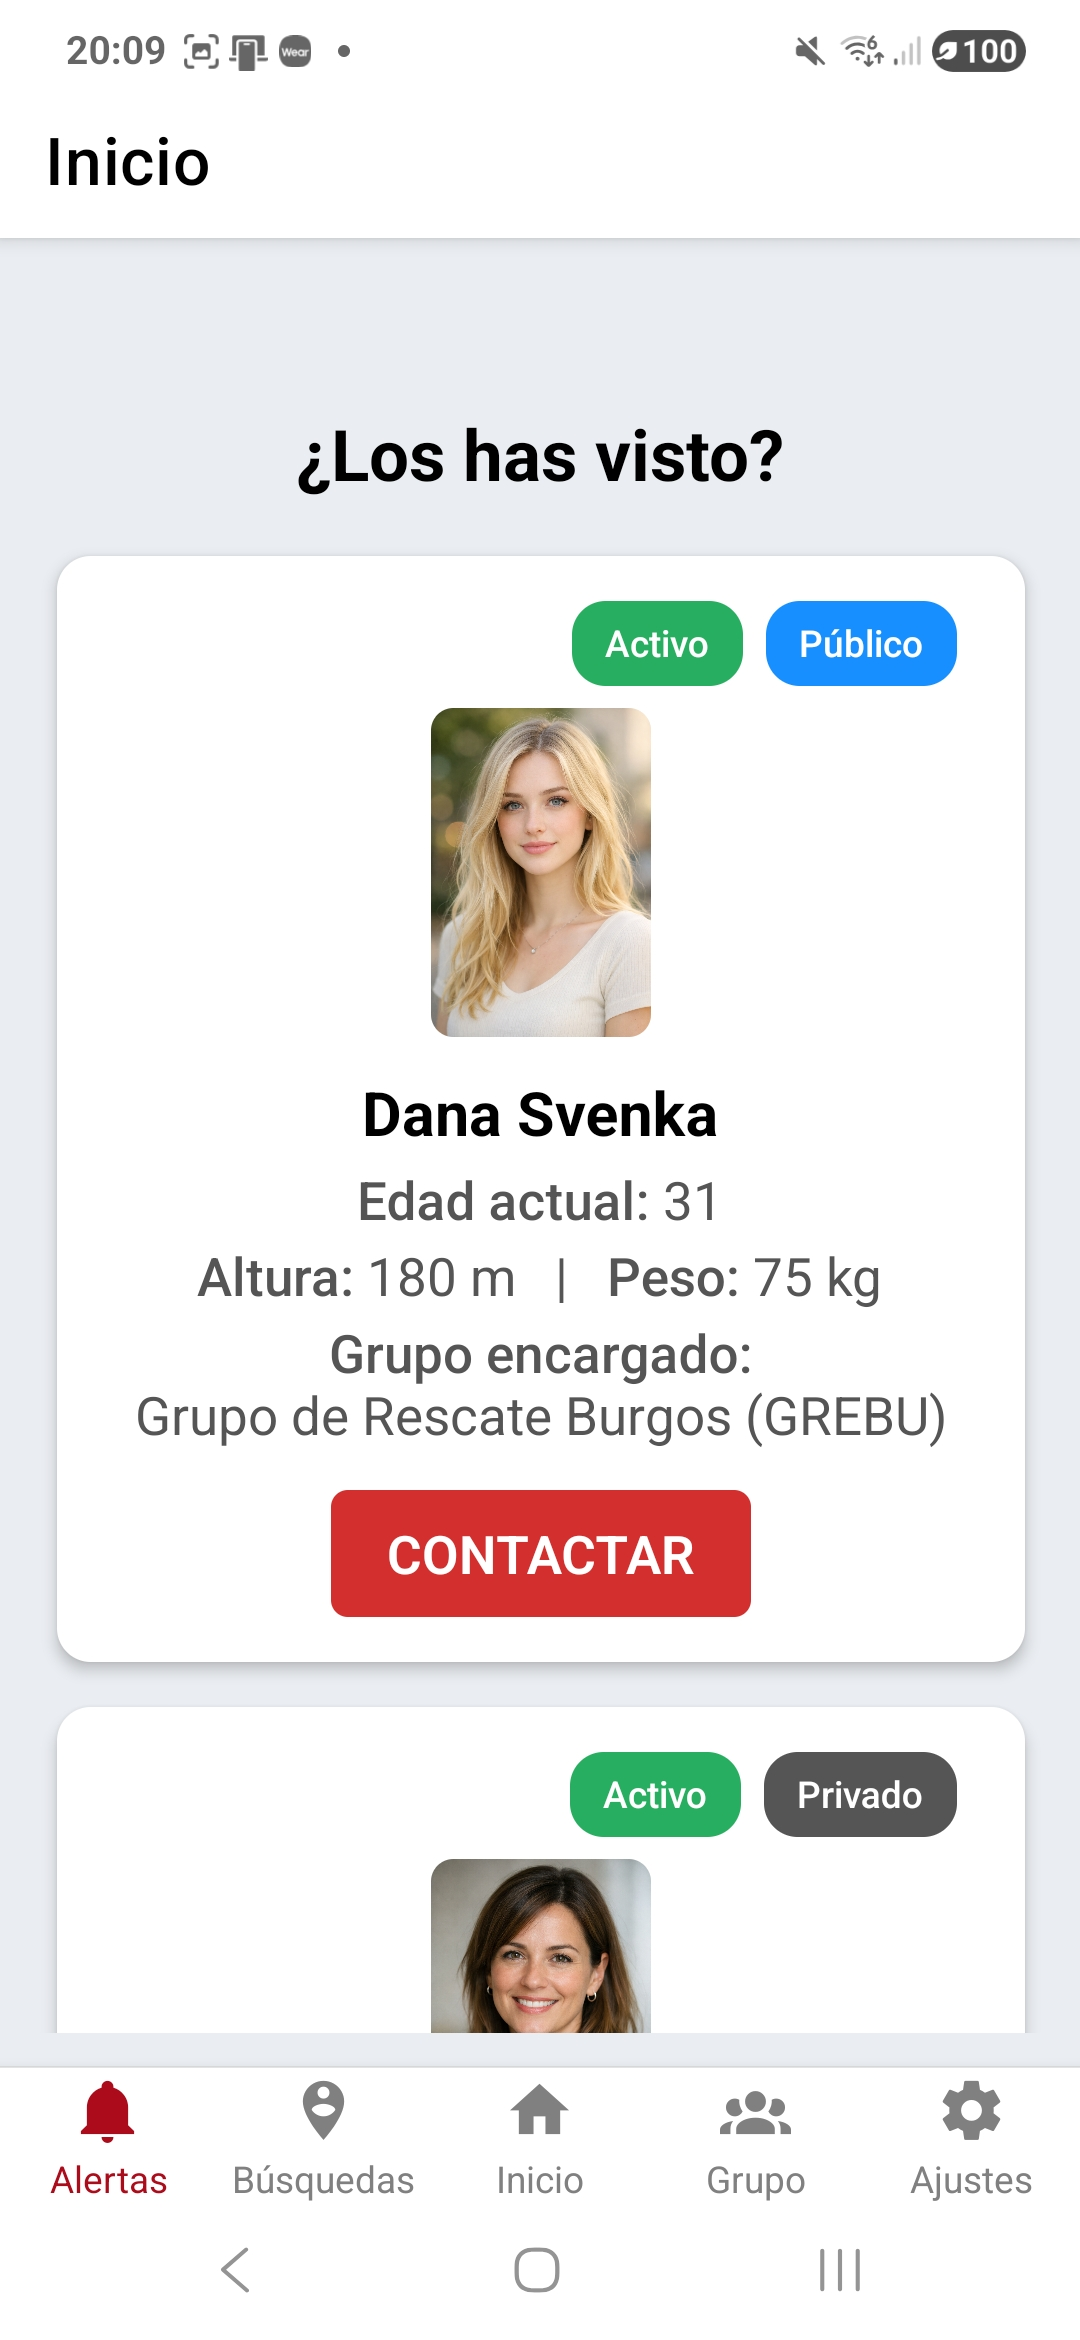
\includegraphics[width=\linewidth]{img/Resultados/Captura_AlertRes_alertasVoluntario.jpg}
            \caption{Voluntarios.}
        \end{subfigure}
        \hfill
        % Segunda imagen
        \begin{subfigure}{0.31\textwidth}
            \centering
            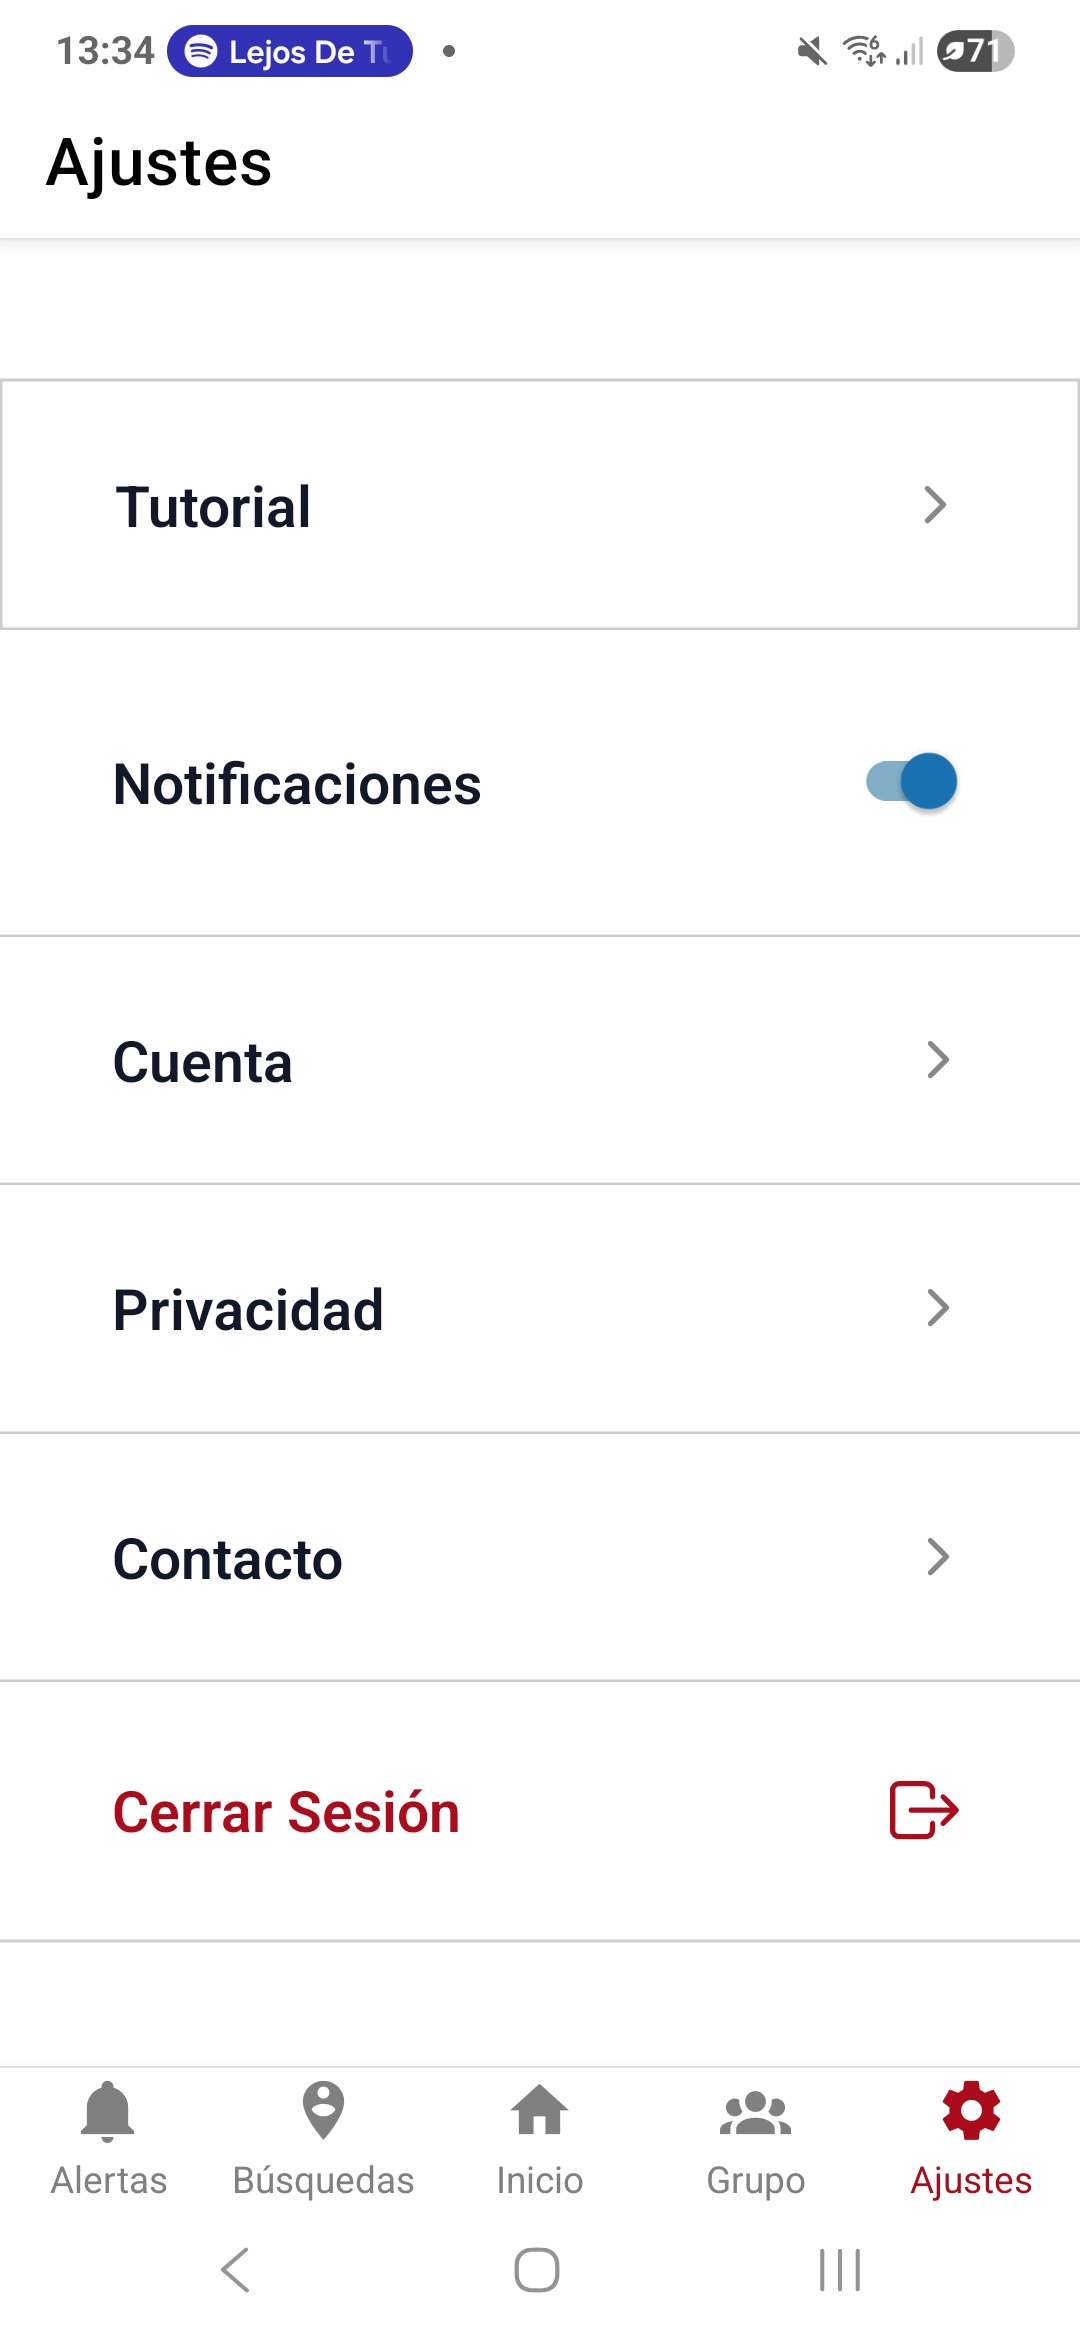
\includegraphics[width=\linewidth]{img/Resultados/Captura_AlertRes_alertas.jpg}
            \caption{Grupos.}
        \end{subfigure}
        \hfill
        % Tercera imagen
        \begin{subfigure}{0.31\textwidth}
            \centering
            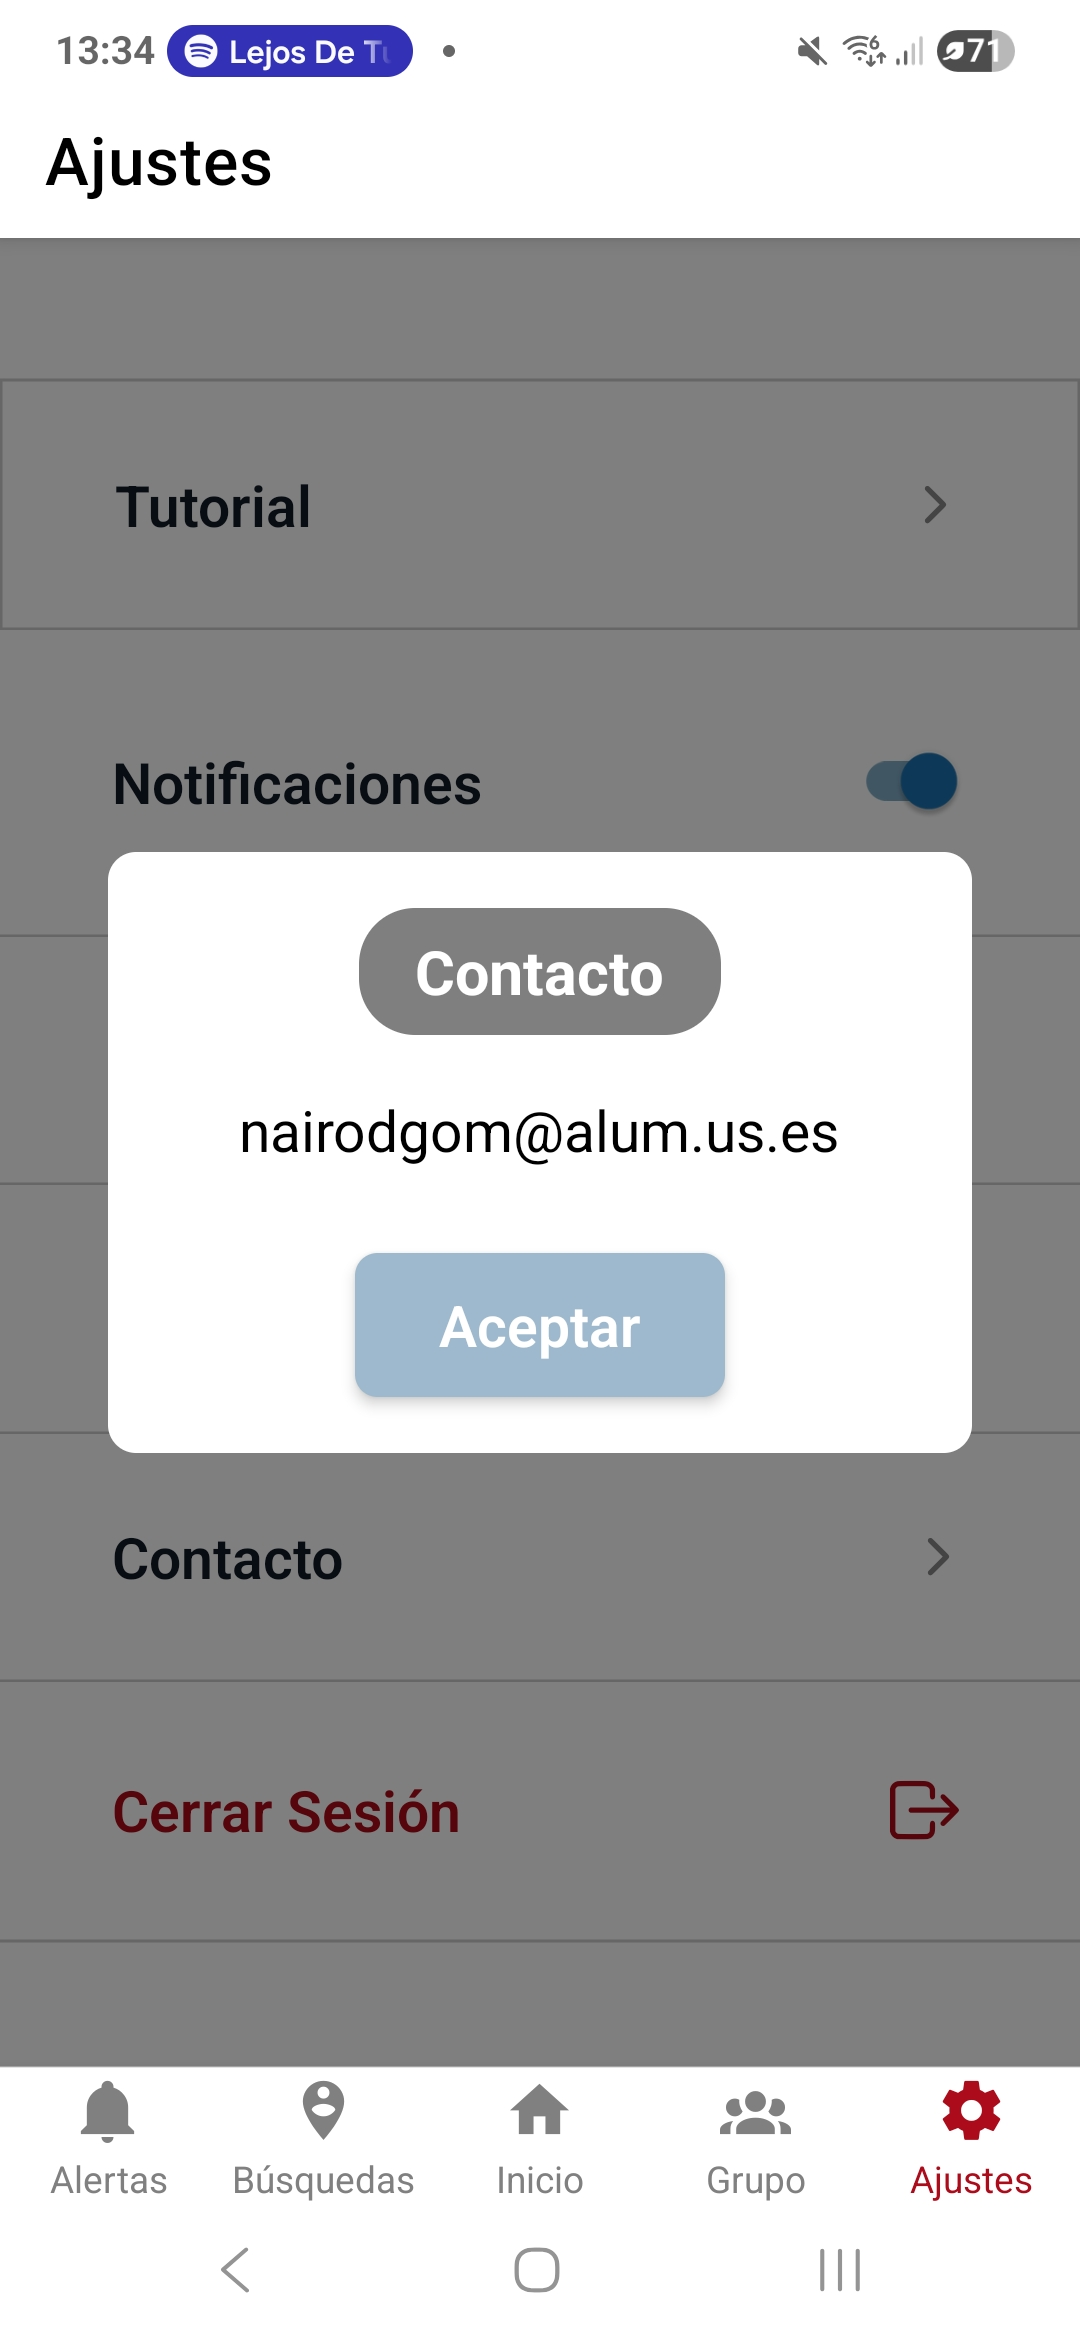
\includegraphics[width=\linewidth]{img/Resultados/Captura_AlertRes_alertasMiembros.jpg}
            \caption{Miembros de grupos.}
        \end{subfigure}
        \hfill
        \caption{Pantalla de alertas. \textit{Fuente propia.}}
        \label{app_alertas}
    \end{figure}


    %\figura{0.35}{img/Resultados/Captura_AlertRes_alertas}{Pantalla de alertas, ejemplo de un usuario grupo. \textit{Fuente propia.}}{app_alertas}{keepaspectratio}
    
    %\figura{0.35}{img/Resultados/Web_AlertaEnviada.png}{Pantalla de alertas para voluntarios. \textit{Fuente propia.}}{app_alertas2}{keepaspectratio}



    \subsubsection{Pantalla de información de una alerta}
    Pantalla que recoge la información básica de la alerta seleccionada para identificación de la persona desaparecida. Además, cuenta con apartado con con la información del grupo responsable y un campo donde poder contactar directamente con los responsables del caso para cualquier comunicación.

    Entre la información que se muestra en esta pantalla se encuentra: la foto del desaparecido, fecha de desaparición, edad actual, última localización conocida, características físicas (altura, peso, color de pelo y de ojos, constitución física...) y etiquetas con el estado del caso y si se trata de una alerta pública o privada.

    Asimismo, esta pantalla cuenta con un botón con el que compartir directamente la alerta por redes sociales.
    
    En la parte inferior se encuentra el menú principal que llevará al resto de pantallas a las que tiene acceso el usuario que ha iniciado sesión.

    \begin{figure}
        \centering
        % Primera imagen
        \begin{subfigure}{0.31\textwidth}
            \centering
            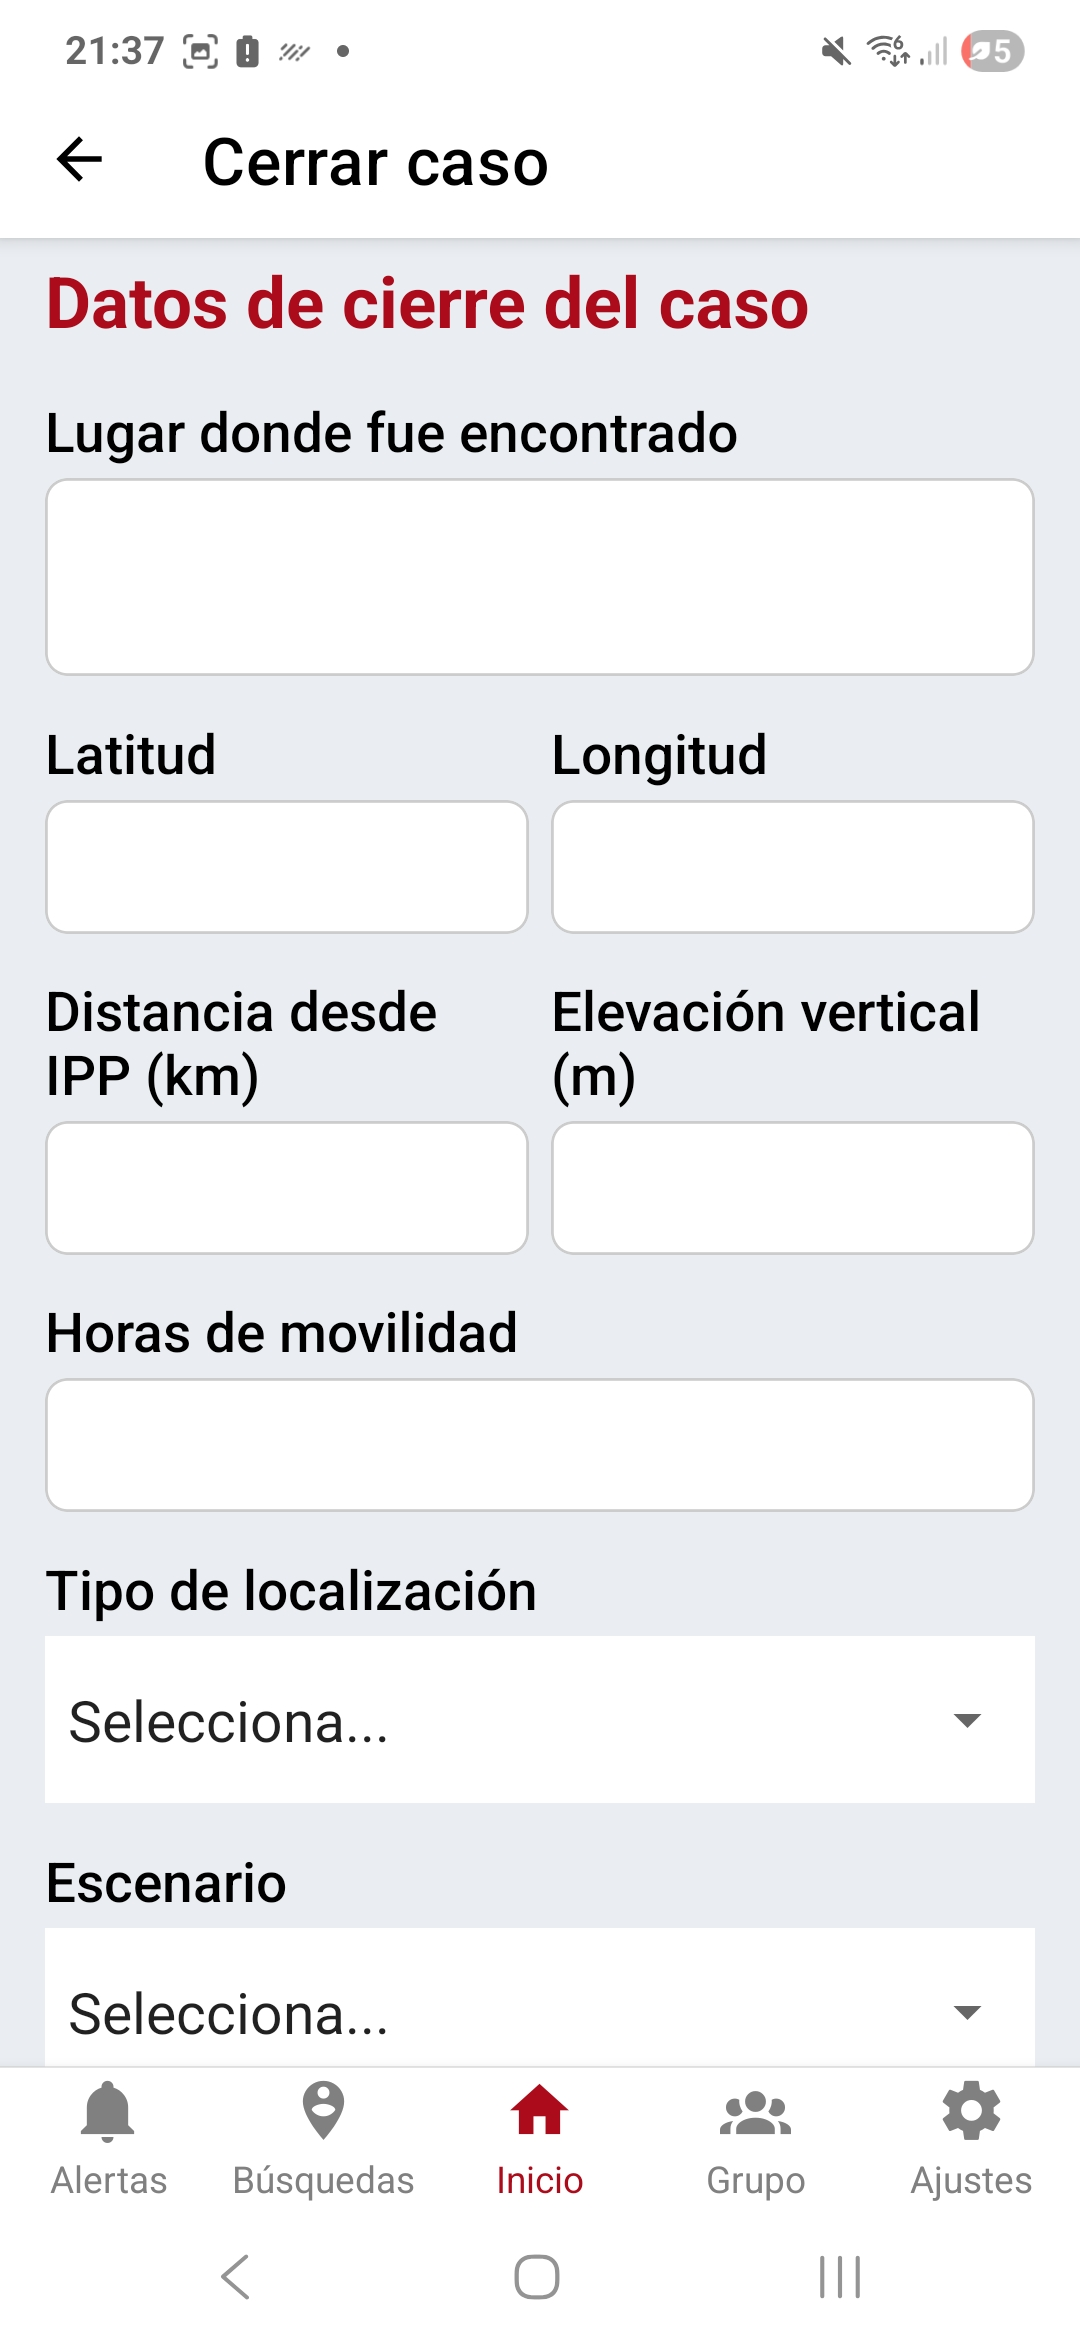
\includegraphics[width=\linewidth]{img/Resultados/Captura_AlertRes_infoAlerta.jpg}
        \end{subfigure}
        \hfill
        % Segunda imagen
        \begin{subfigure}{0.31\textwidth}
            \centering
            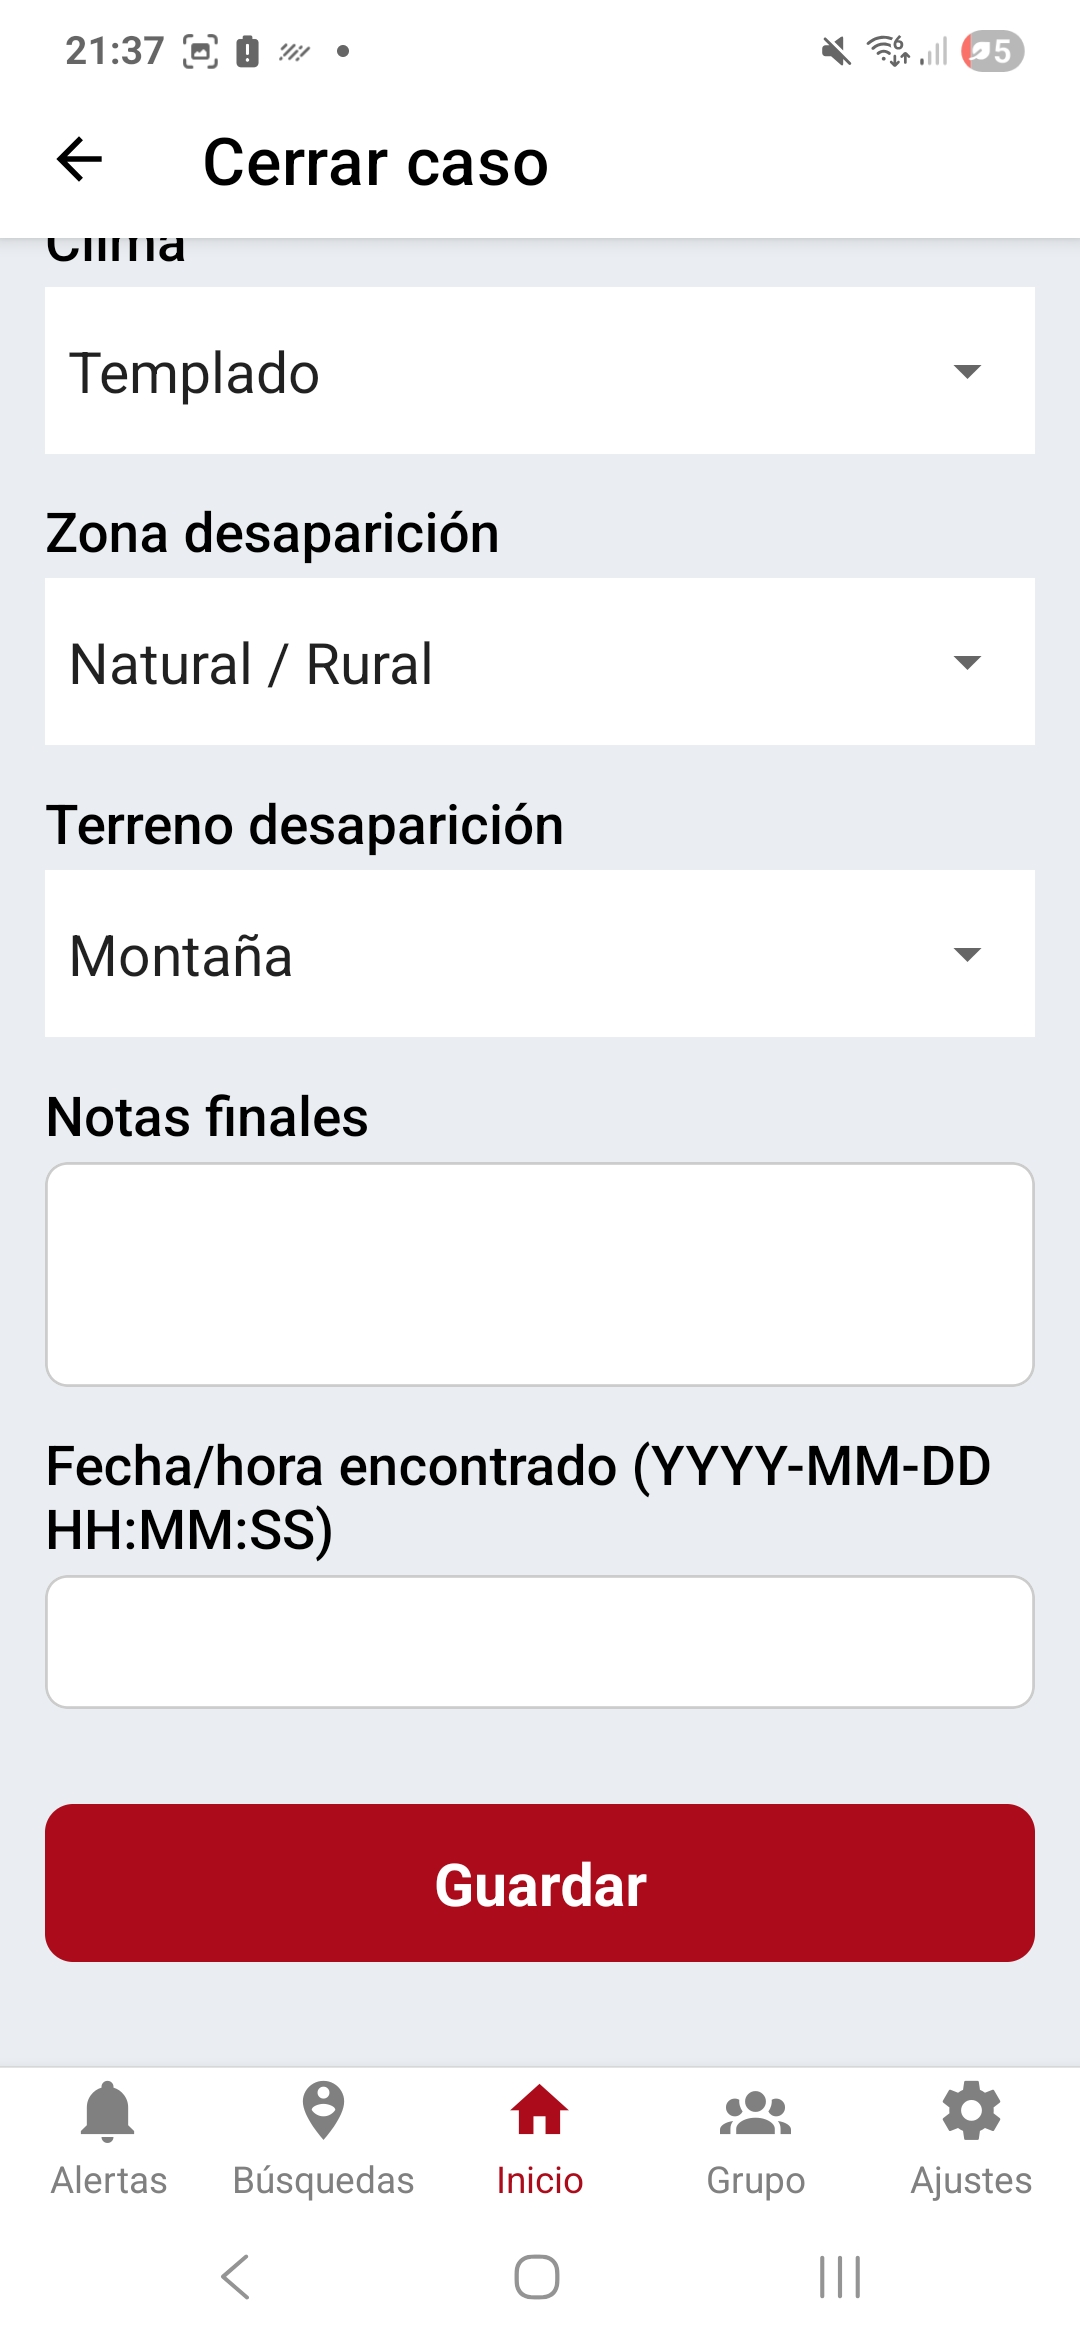
\includegraphics[width=\linewidth]{img/Resultados/Captura_AlertRes_infoAlerta2.jpg}
        \end{subfigure}
        \hfill
        % Tercera imagen
        \begin{subfigure}{0.31\textwidth}
            \centering
            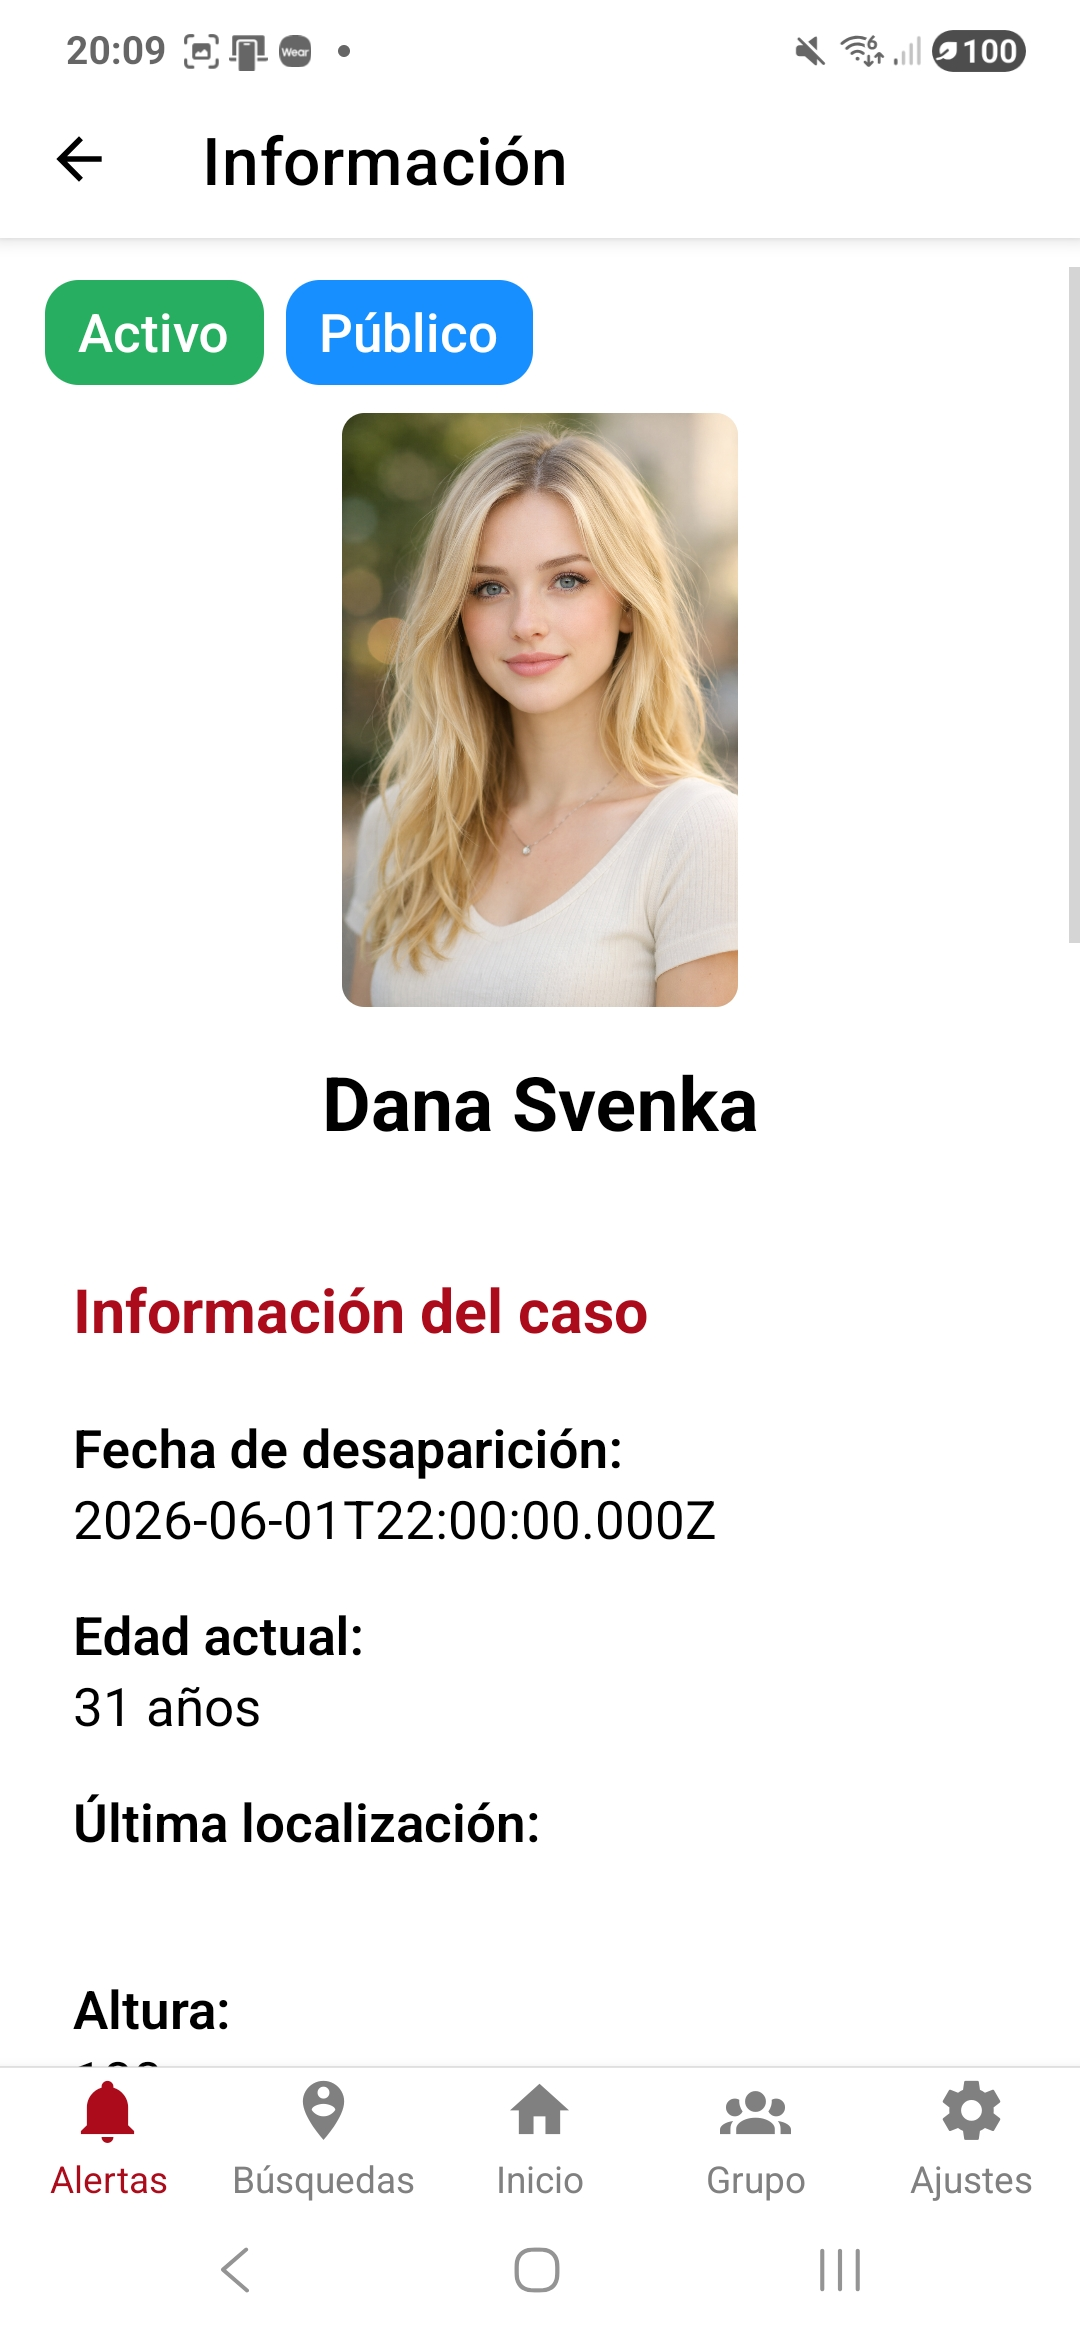
\includegraphics[width=\linewidth]{img/Resultados/Captura_AlertRes_infoAlerta3.jpg}
        \end{subfigure}
        \hfill
        \caption{Pantalla de información de una alerta. \textit{Fuente propia.}}
        \label{app_infoAlerta}
    \end{figure}

    %\figura{0.35}{img/Resultados/Web_AlertaEnviada.png}{Pantalla de información de una alerta. \textit{Fuente propia.}}{app_infoAlerta}{keepaspectratio}



    \subsubsection{Pantalla de búsquedas}

    Pantalla que recoge una lista con todas las búsquedas activas actualmente. Esta lista se obtiene desde el backend con una serie de solicitudes tipo GET a las distintas tablas, siendo la principal la tabla \texttt{searches}.
    
    En función del rol del usuario se tendrá acceso únicamente a búsquedas públicas o, en caso de pertenecer a un grupo, las búsquedas privadas del mismo. 

    Cada búsqueda estará identificada con el nombre de la persona desaparecida, el lugar donde se llevará a cabo y la fecha de creación de la misma. Además, también cuentan con dos etiquetas informativas:
    \begin{itemize}
        \item Una etiqueta relativa al estado siendo verde si se encuentra activa o roja si está cerrada.
        \item Otra relativa a la visibilidad, que puede ser naranja si es pública o gris si es privada  Además, también se indica el grupo encargado de la búsqueda.
    \end{itemize}

    En caso de seleccionar una búsqueda la aplicación abrirá un modal de inscripción a esa búsqueda (\textit{Ver Imagen \ref{app_busquedasmodal}}), en caso de aceptar quedará registrado en la base de datos, en la tabla \texttt{search participants} y navegará a la pantalla de información de la búsqueda especificada. Una vez aceptado participar en una búsqueda no volverá a salir el modal para esa búsqueda. Además, se incrementará el contador de participaciones en búsquedas con el que cuentan todos los usuarios.

    Como en el resto de pantallas, en la parte inferior se encuentra el menú principal que permite navegar al resto de pantallas a las que tiene acceso el usuario que ha iniciado sesión.

    \begin{figure}[h!]
        \centering
        % Primera imagen
        \begin{subfigure}{0.31\textwidth}
            \centering
            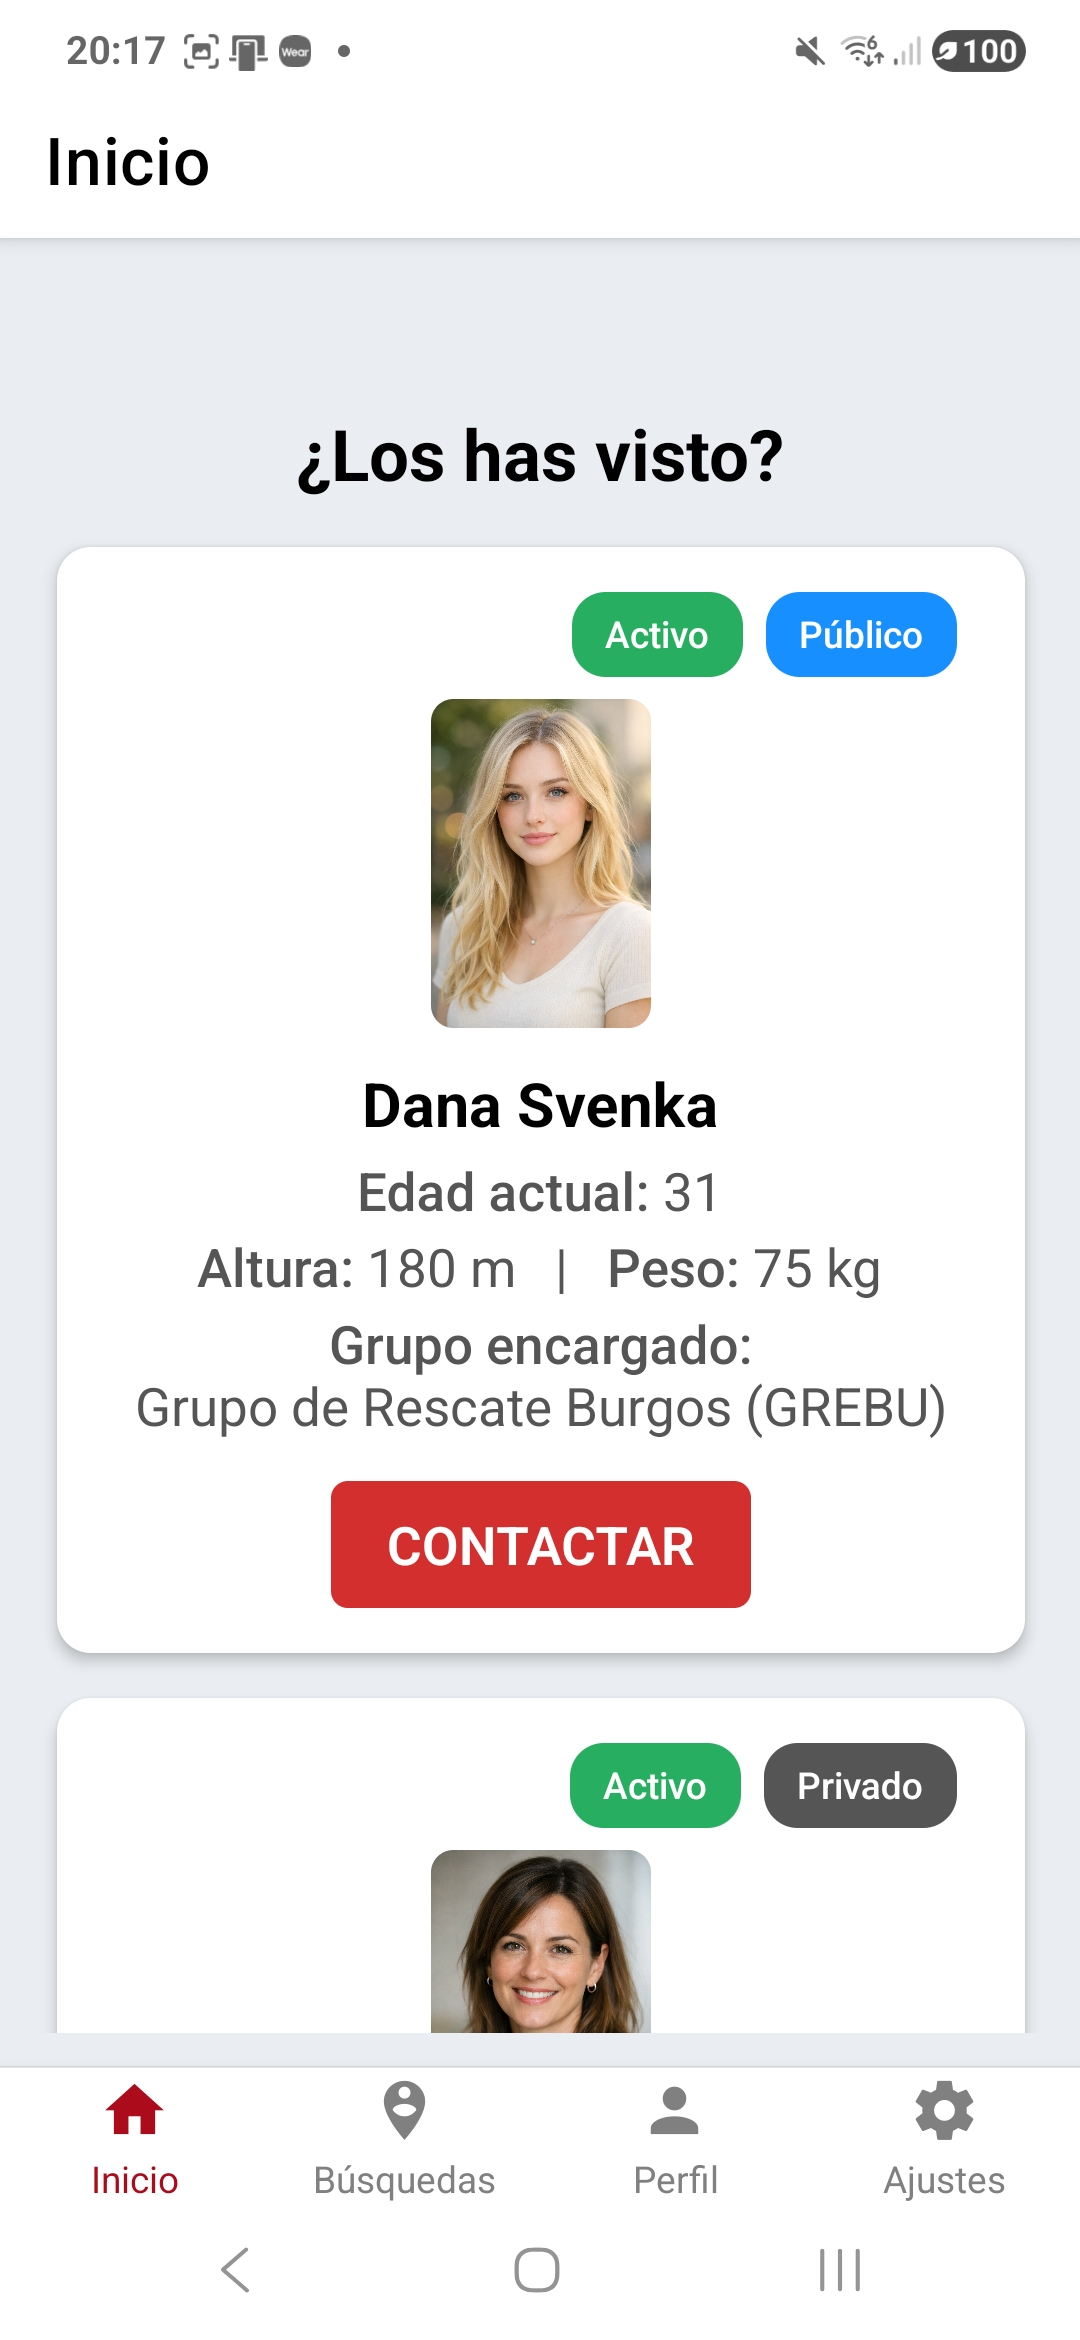
\includegraphics[width=\linewidth]{img/Resultados/Captura_AlertRes_busquedas.jpg}
            \caption{Grupos.}
        \end{subfigure}
        \hfill
        % Segunda imagen
        \begin{subfigure}{0.31\textwidth}
            \centering
            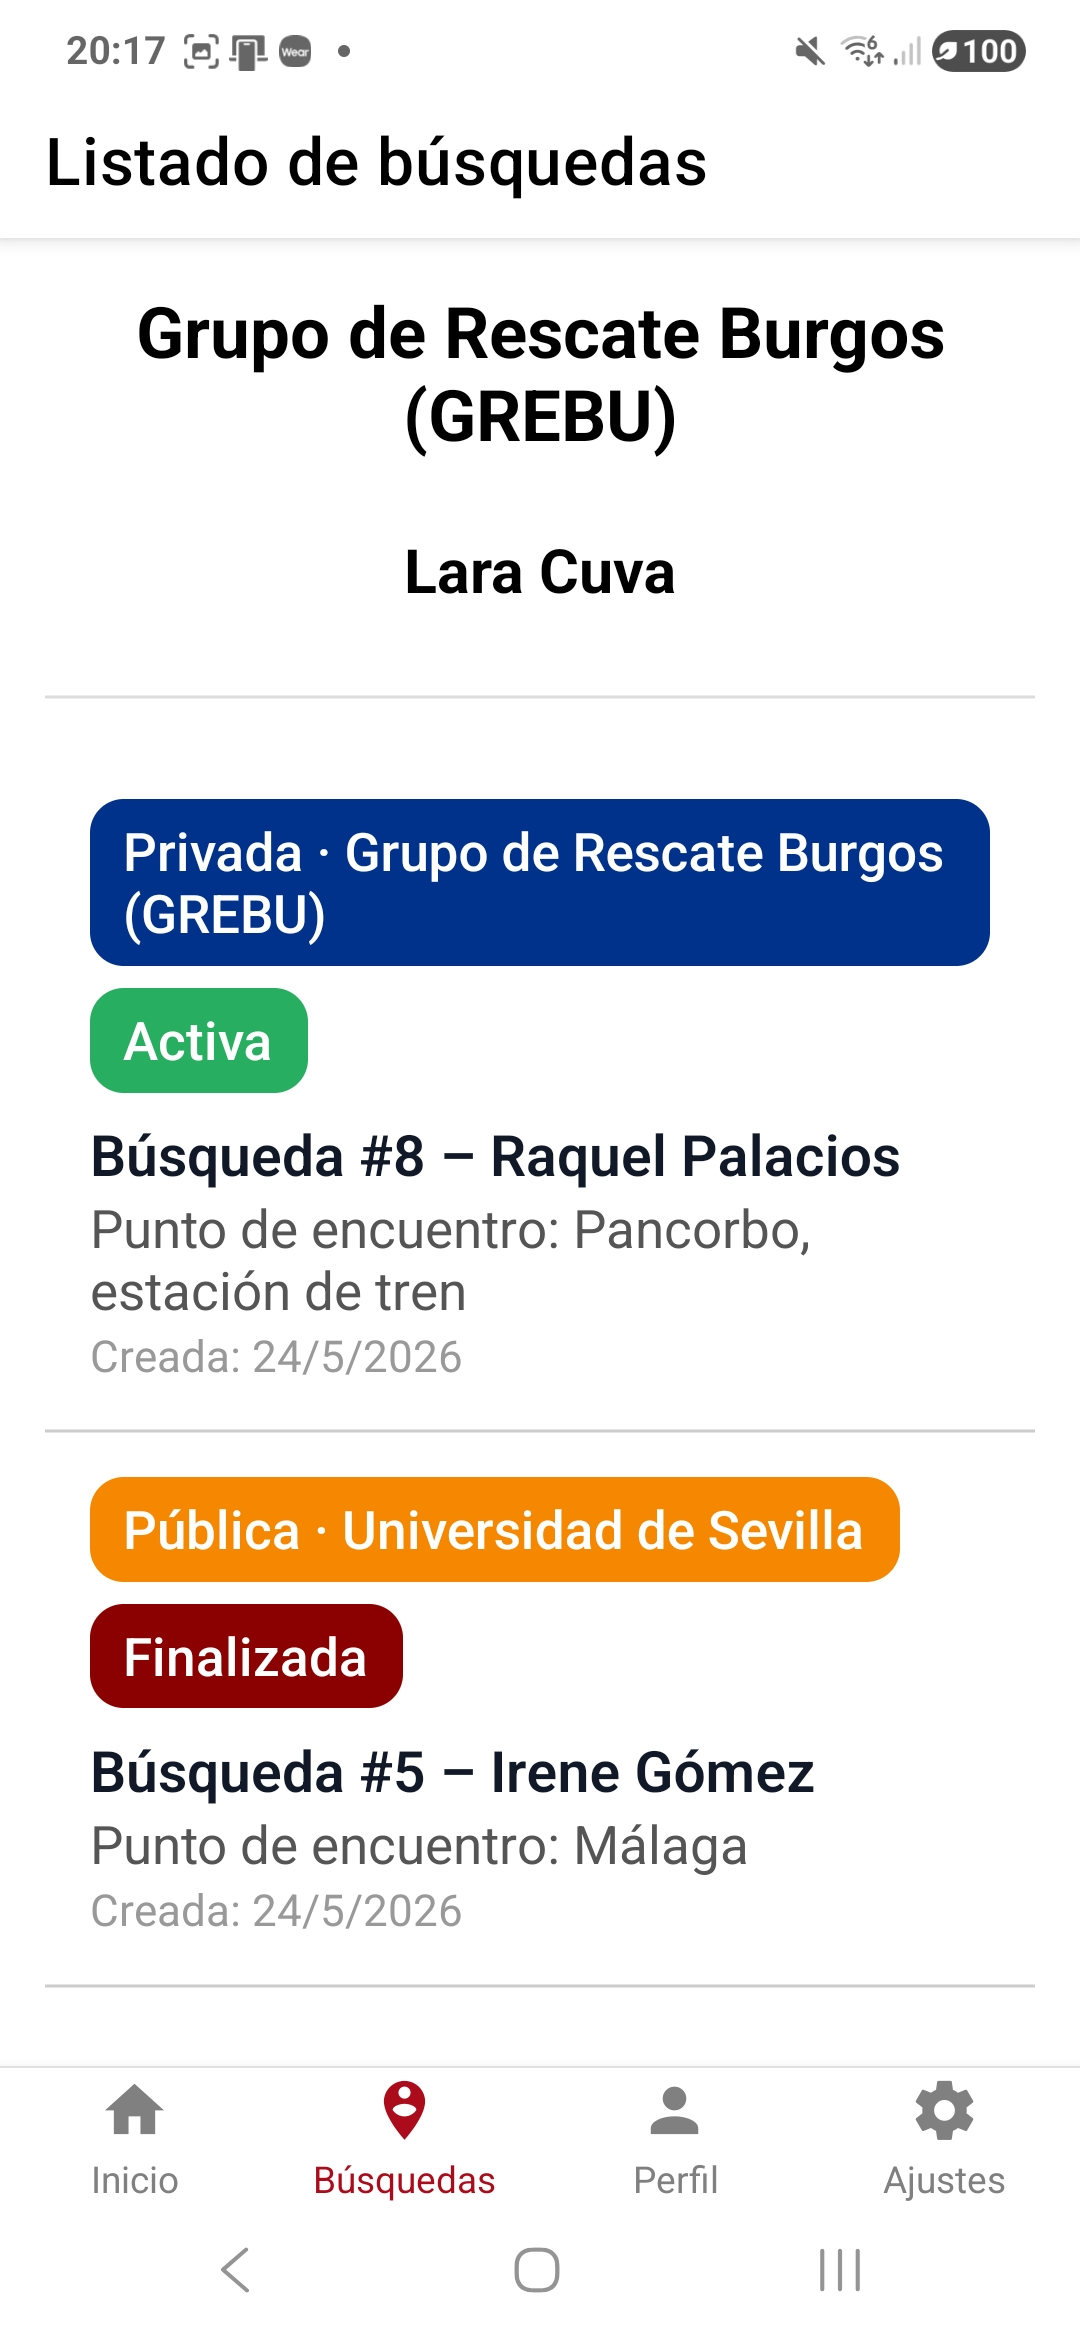
\includegraphics[width=\linewidth]{img/Resultados/Captura_AlertRes_busquedasVoluntario.jpg}
            \caption{Voluntarios.}
        \end{subfigure}
        \hfill
        % Tercera imagen
        \begin{subfigure}{0.31\textwidth}
            \centering
            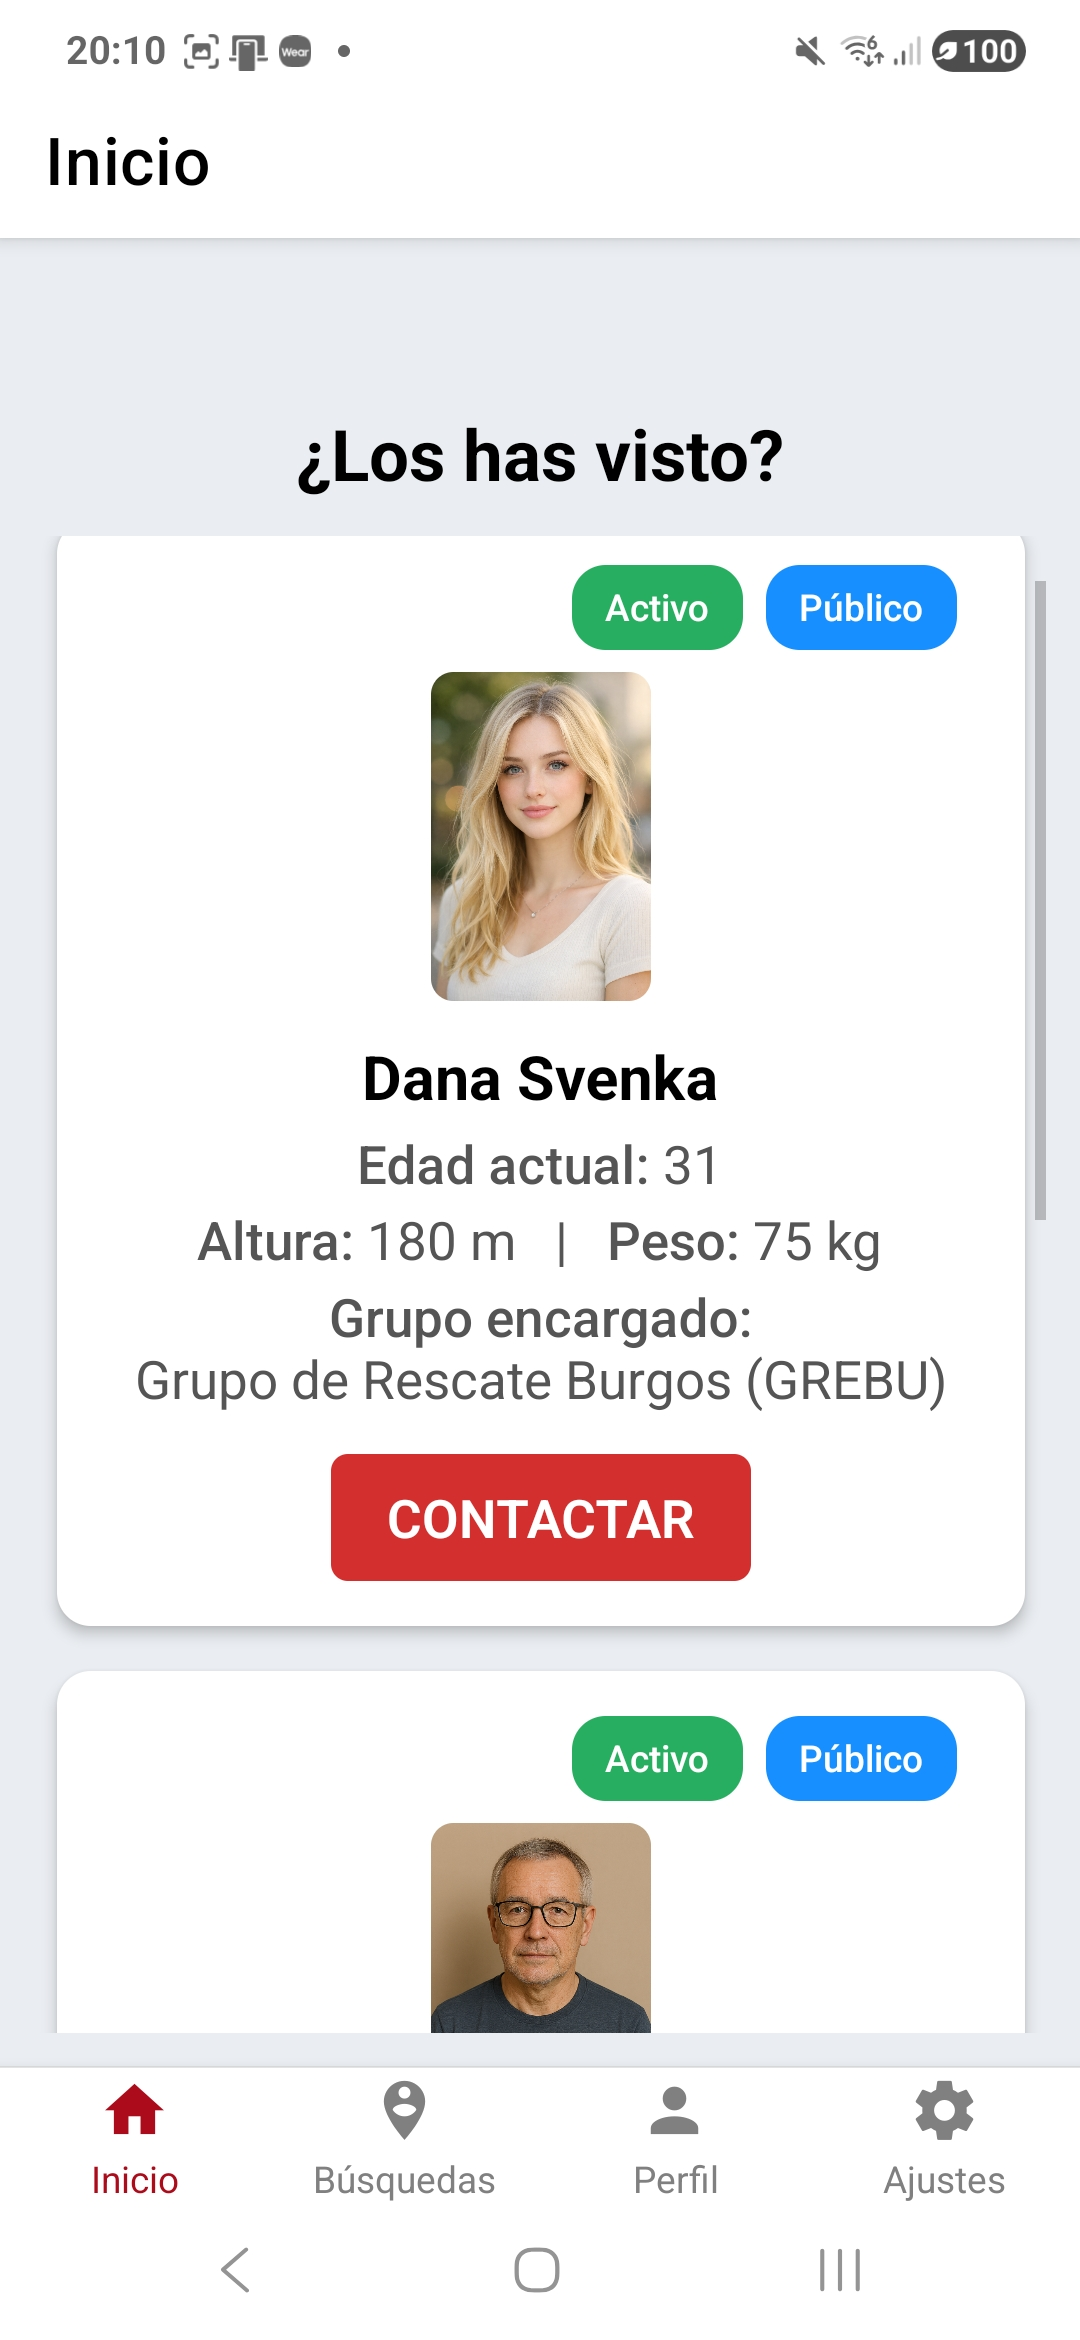
\includegraphics[width=\linewidth]{img/Resultados/Captura_AlertRes_busquedasMiembro.jpg}
            \caption{Miembros de grupos.}
        \end{subfigure}
        \caption{Pantalla con el listado de búsquedas en las que puede participar el usuario. \textit{Fuente propia.}}
        \label{app_busquedas}
    \end{figure}

    %\figura{0.35}{img/Resultados/Captura_AlertRes_busquedas.jpg}{Pantalla con el listado de búsquedas en las que puede participar el usuario. \textit{Fuente propia.}}{app_busquedas}{keepaspectratio}

    \begin{figure}[h!]
        \centering
        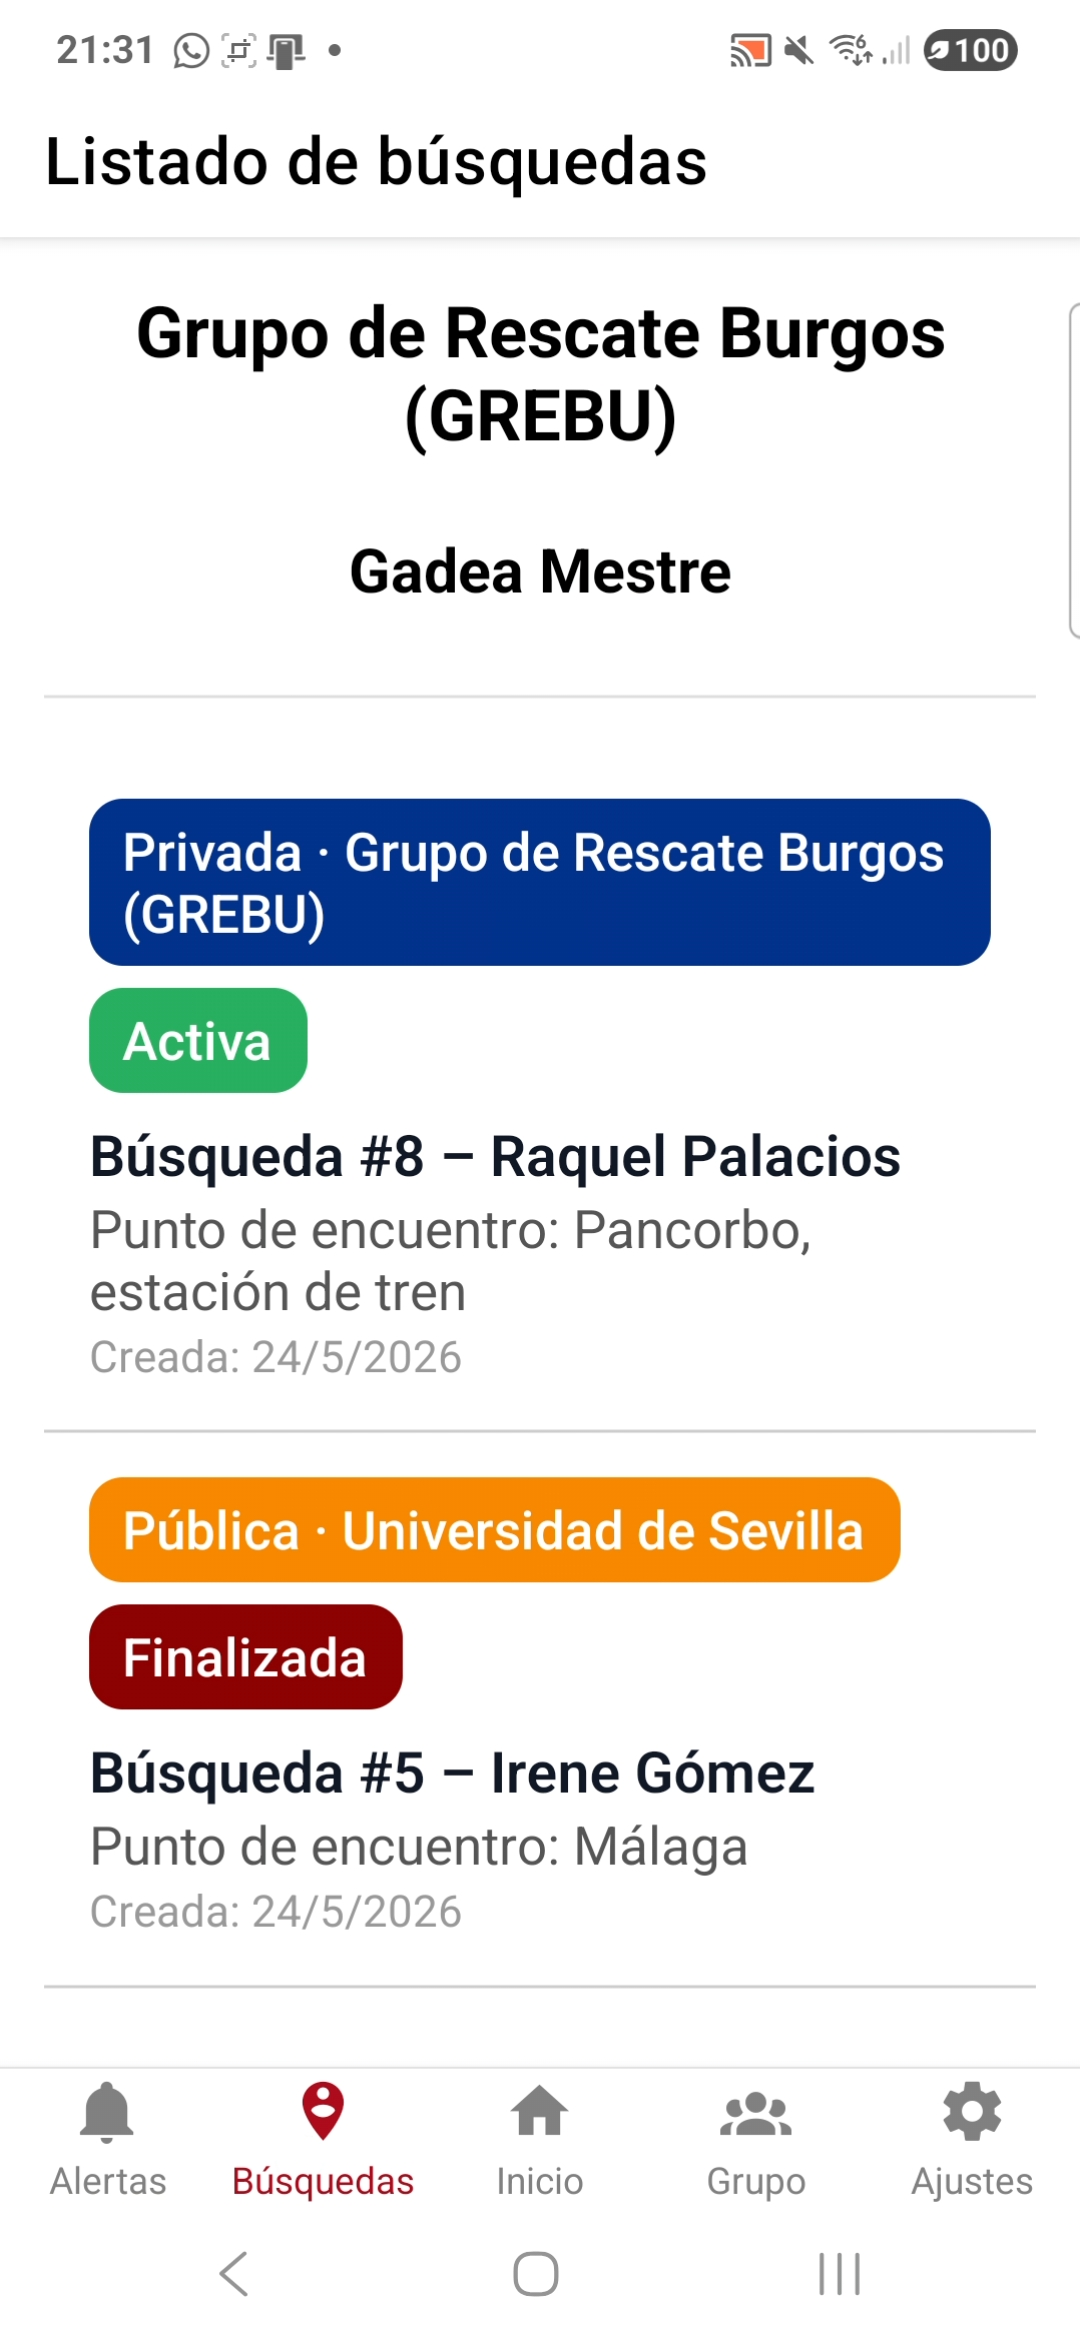
\includegraphics[width=0.26\linewidth]{img/Resultados/Captura_AlertRes_busquedasModal.jpg}
        \caption{Pantalla con el modal de aceptación en participación de una búsqueda. \textit{Fuente propia.}}
        \label{app_busquedasmodal}
    \end{figure}

    %\figura{0.31}{img/Resultados/Captura_AlertRes_busquedasModal.jpg}{Pantalla con el modal de aceptación en participación de una búsqueda. \textit{Fuente propia.}}{app_busquedasmodal}{keepaspectratio}



    \subsubsection{Pantalla de información de una búsqueda}

    Aquí se recoge toda la información relativa a la búsqueda.
 
    Se pueden diferenciar 4 campos principales:
    \begin{itemize}
        \item Información del desaparecido: nombre y apellidos, edad y otras características esenciales para su identificación.

        \item Botón de acceso al mapa que se activará una vez se de comienzo a la búsqueda y donde se podrá acceder a todo lo relacionado con la geolocalización de los participantes. Aunque, esta funcionalidad no se ha llegado a implementar correctamente por incopatibilidades con Expo Go y web.

        \item Información específica de la búsqueda, como el punto de encuentro, la fecha de realización de la búsqueda o el grupo organizador de la misma.

        \item Un modal de recomendaciones para todos los participantes en la búsqueda.
        
    \end{itemize}

    En la parte inferior se encuentra el menú principal que llevará al resto de pantallas a las que tiene acceso el usuario que ha iniciado sesión.
    
    \begin{figure}[h!]
        \centering
        % Primera imagen
        \begin{subfigure}{0.65\textwidth}
            \centering
            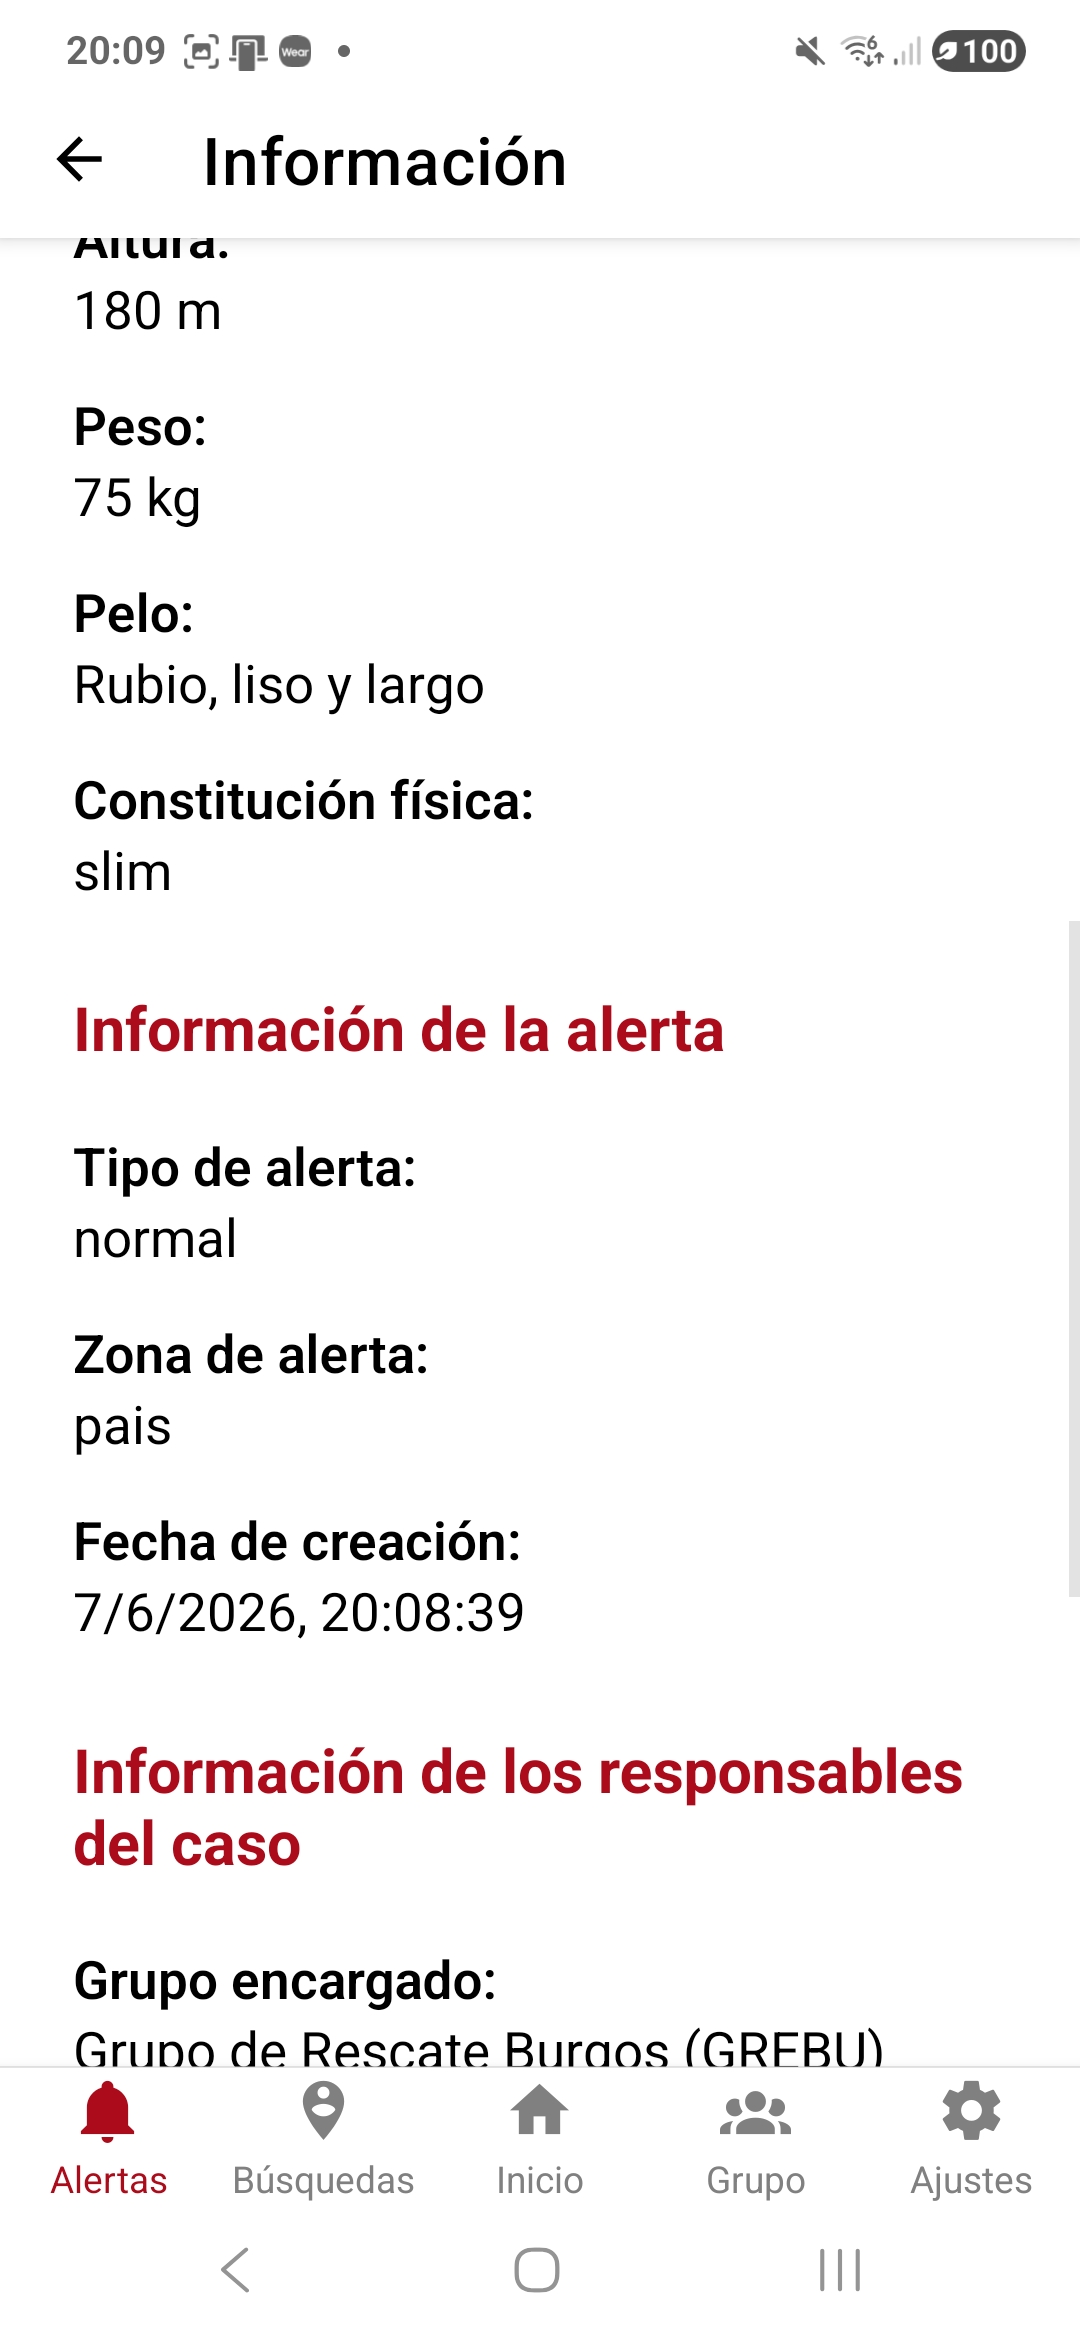
\includegraphics[width=0.49\linewidth]{img/Resultados/Captura_AlertRes_infoBusqueda.jpg}
            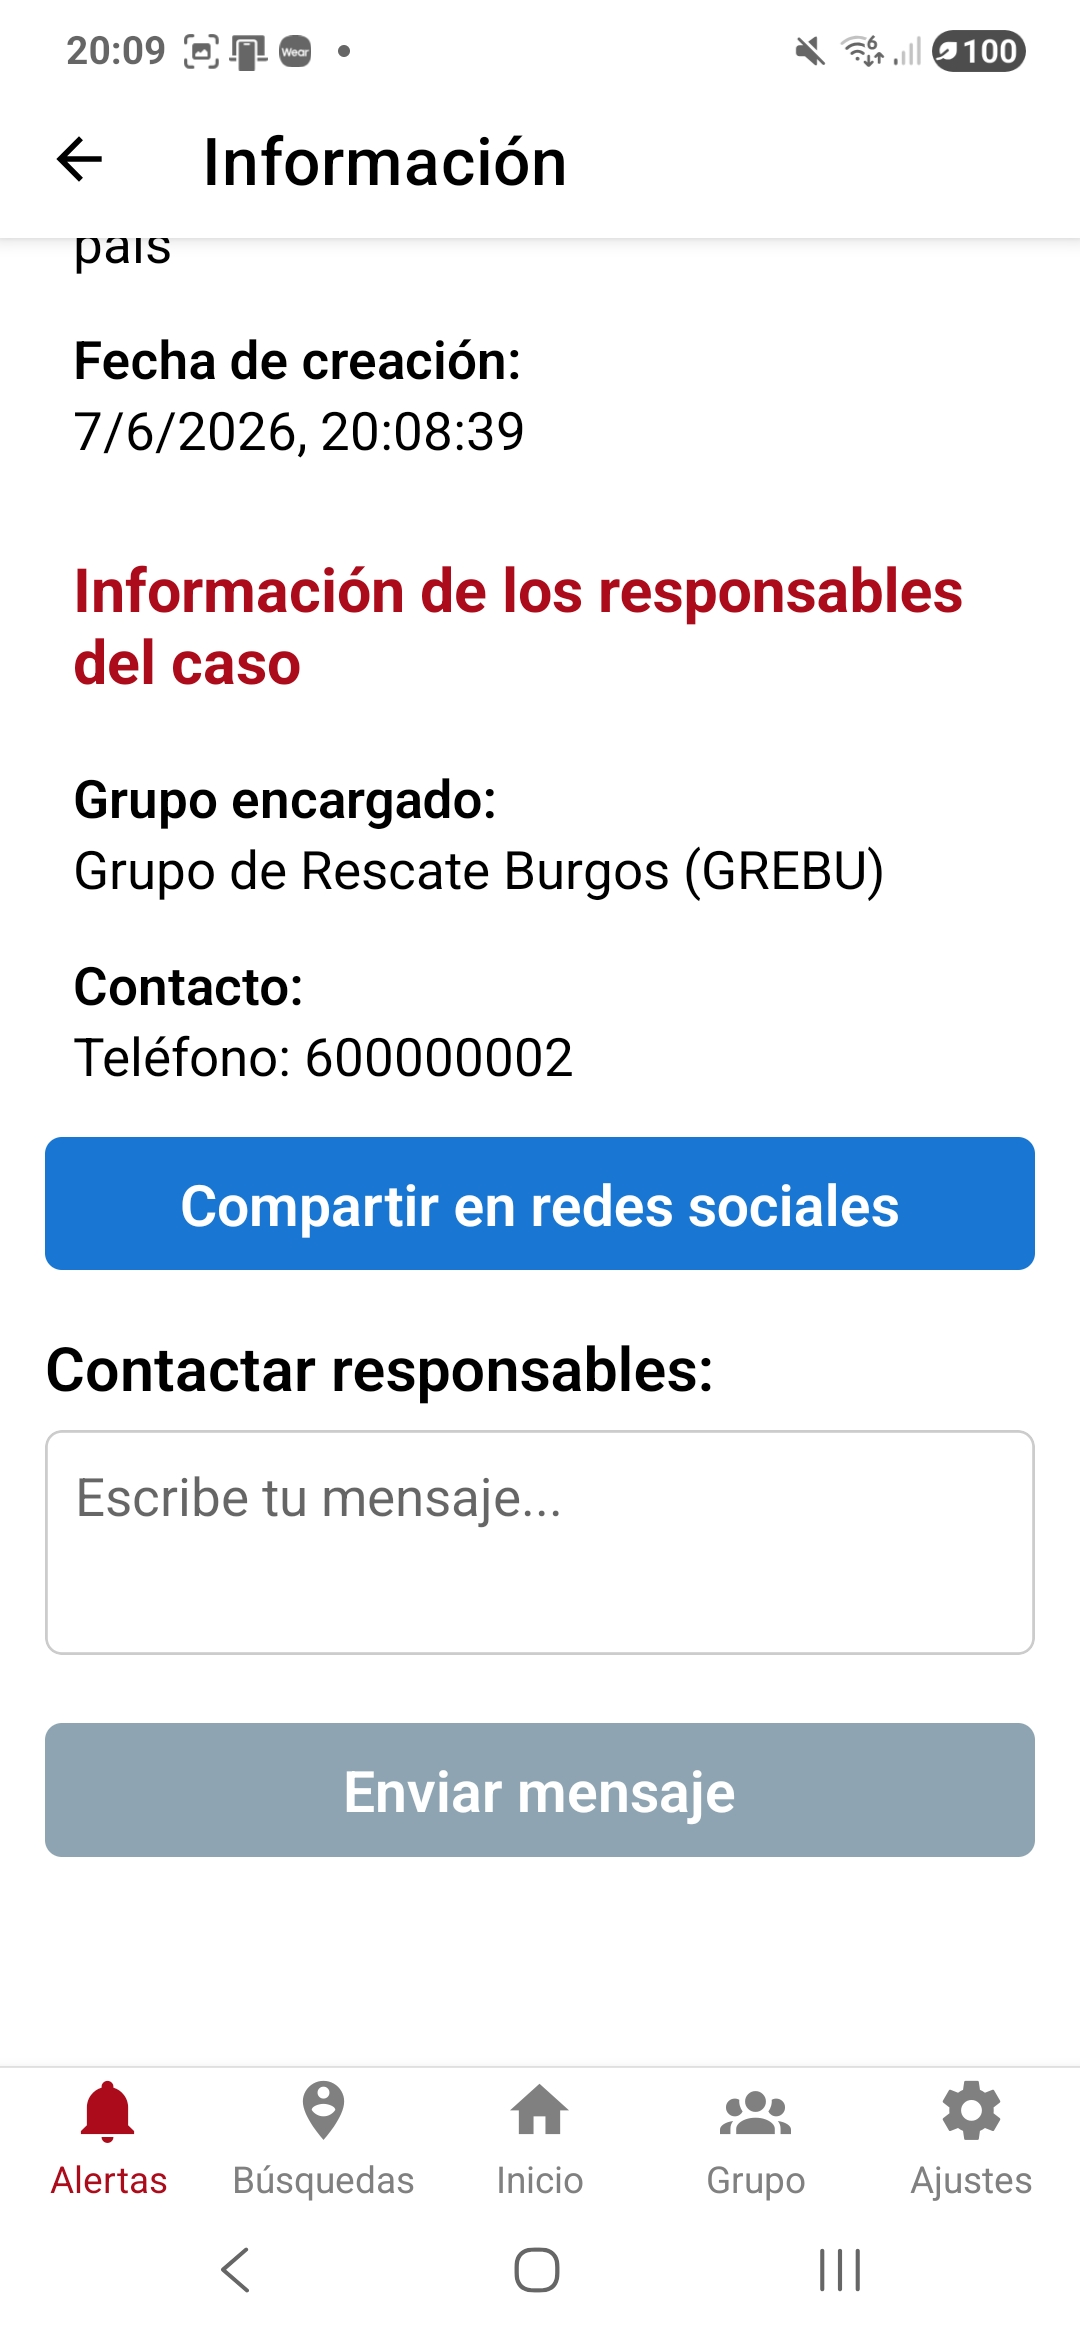
\includegraphics[width=0.49\linewidth]{img/Resultados/Captura_AlertRes_infoBusqueda2.jpg}
            \caption{Información de una búsqueda.}
        \end{subfigure}
        \hfill
        % Tercera imagen
        \begin{subfigure}{0.31\textwidth}
            \centering
            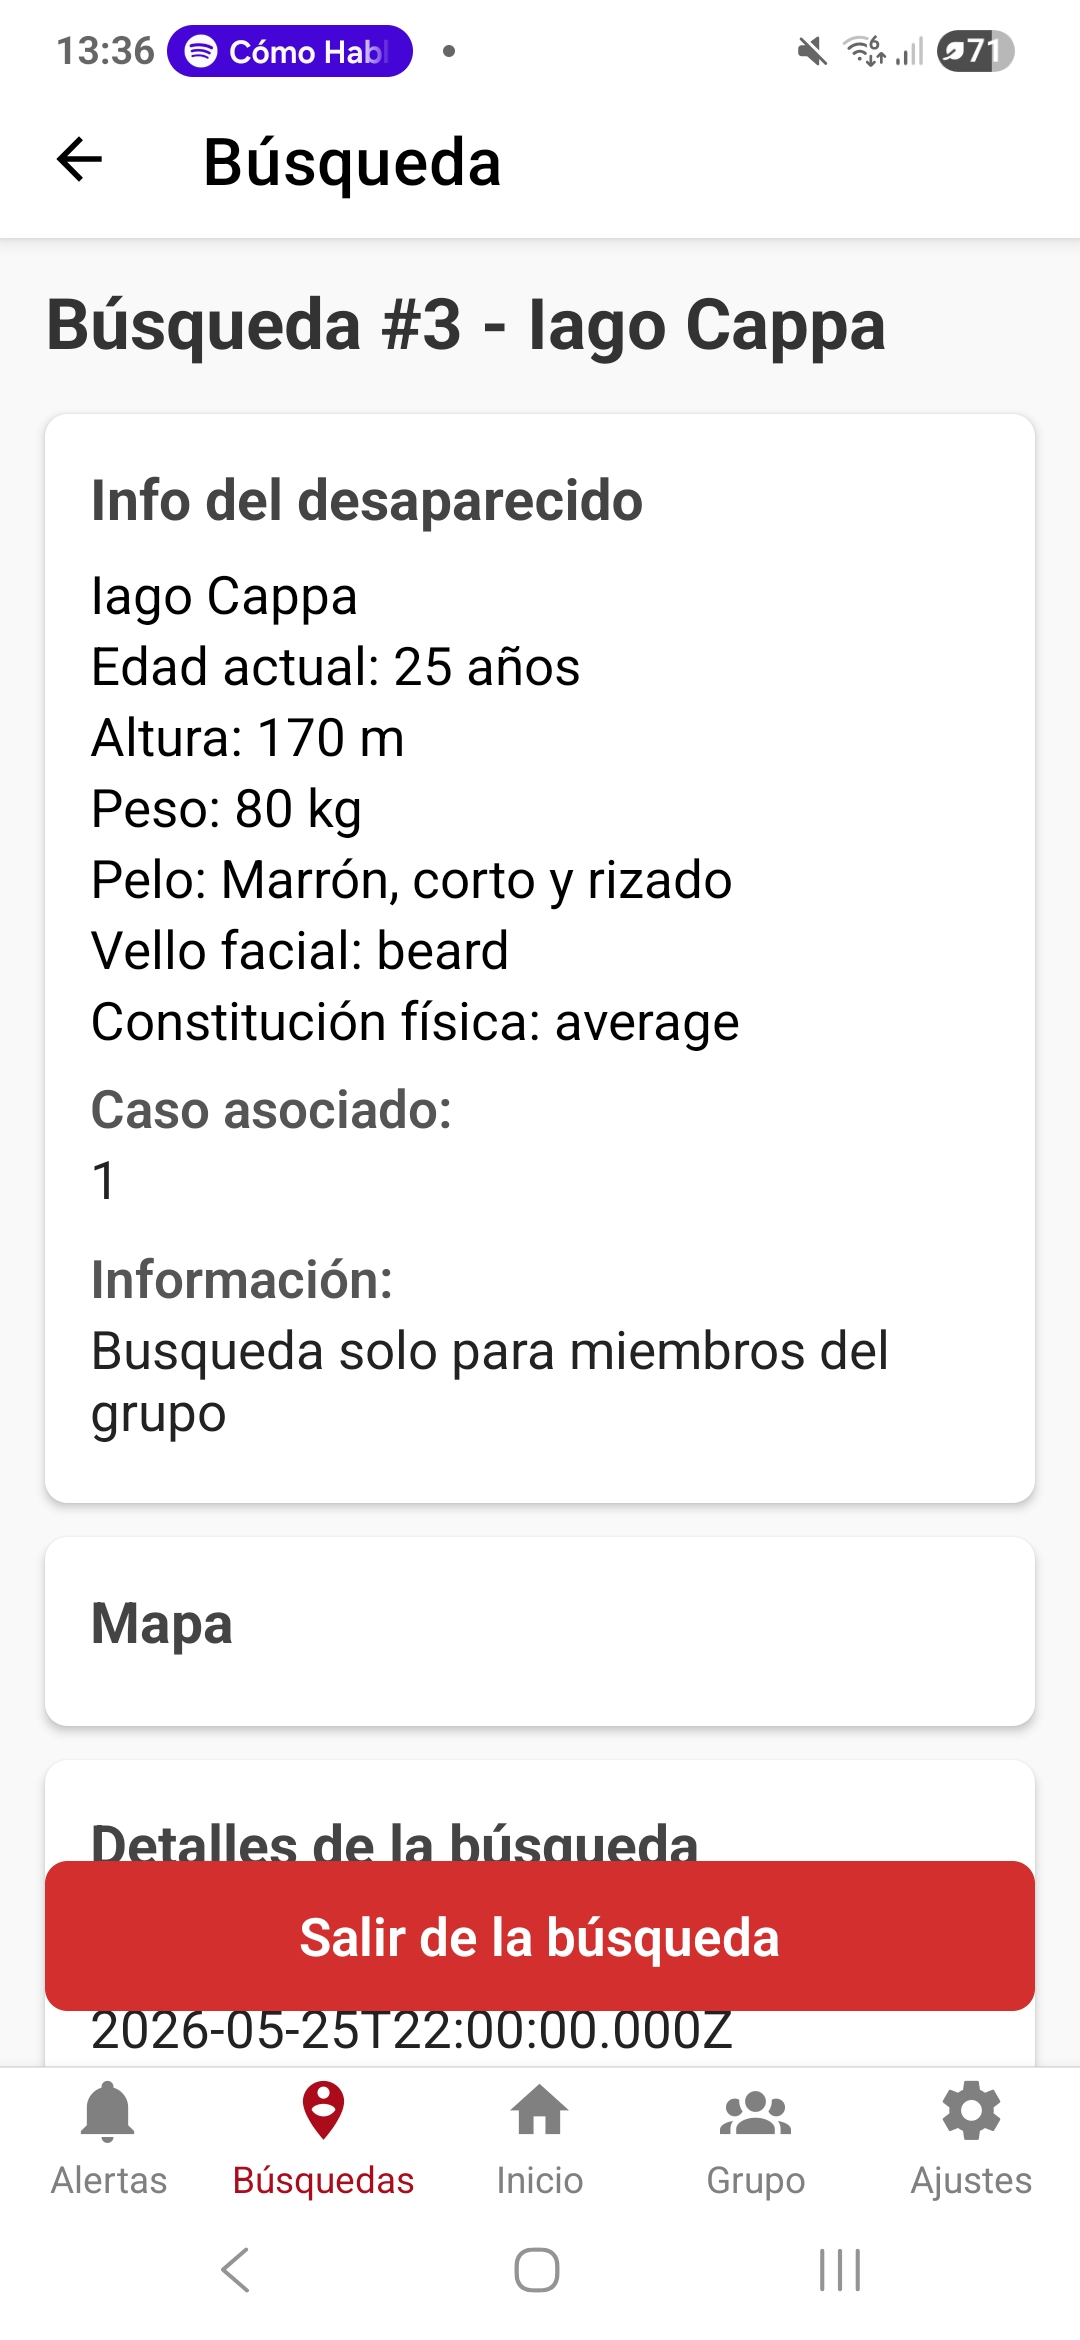
\includegraphics[width=\linewidth]{img/Resultados/Captura_AlertRes_infoBusquedaModal.jpg}
            \caption{Modal de recomendaciones para una búsqueda.}
        \end{subfigure}
        \caption{Pantalla de información de una búsqueda. \textit{Fuente propia.}}
        \label{app_infoBusqueda}
    \end{figure}


    \subsubsection{Pantalla con información del grupo}

    Esta pantalla recoge la información del grupo que ha iniciado sesión. En concreto, se presenta el nombre del grupo y de la persona encargada y semuestra una lista con todos los miembros actualmente registrados pertenecientes al grupo. 

    Por otro lado, esta pantalla cuenta con un botón para añadir miembros. Una vez se presione sobre el botón saltará un modal en la pantalla donde poder introducir el DNI y el rol del miembro del grupo que se quiera añadir.

    Toda la información relativa a los miembros se obtiene con solicitudes GET en las tablas de la base de datos de AlertRes: \texttt{group members}, \texttt{rescue groups}, \texttt{users} y \texttt{people}.
    
    En la parte inferior se encuentra el menú principal que llevará al resto de pantallas a las que tiene acceso el usuario que ha iniciado sesión con rol de grupo.

    \begin{figure}[h!]
        \centering
        % Primera imagen
        \begin{subfigure}{0.36\textwidth}
            \centering
            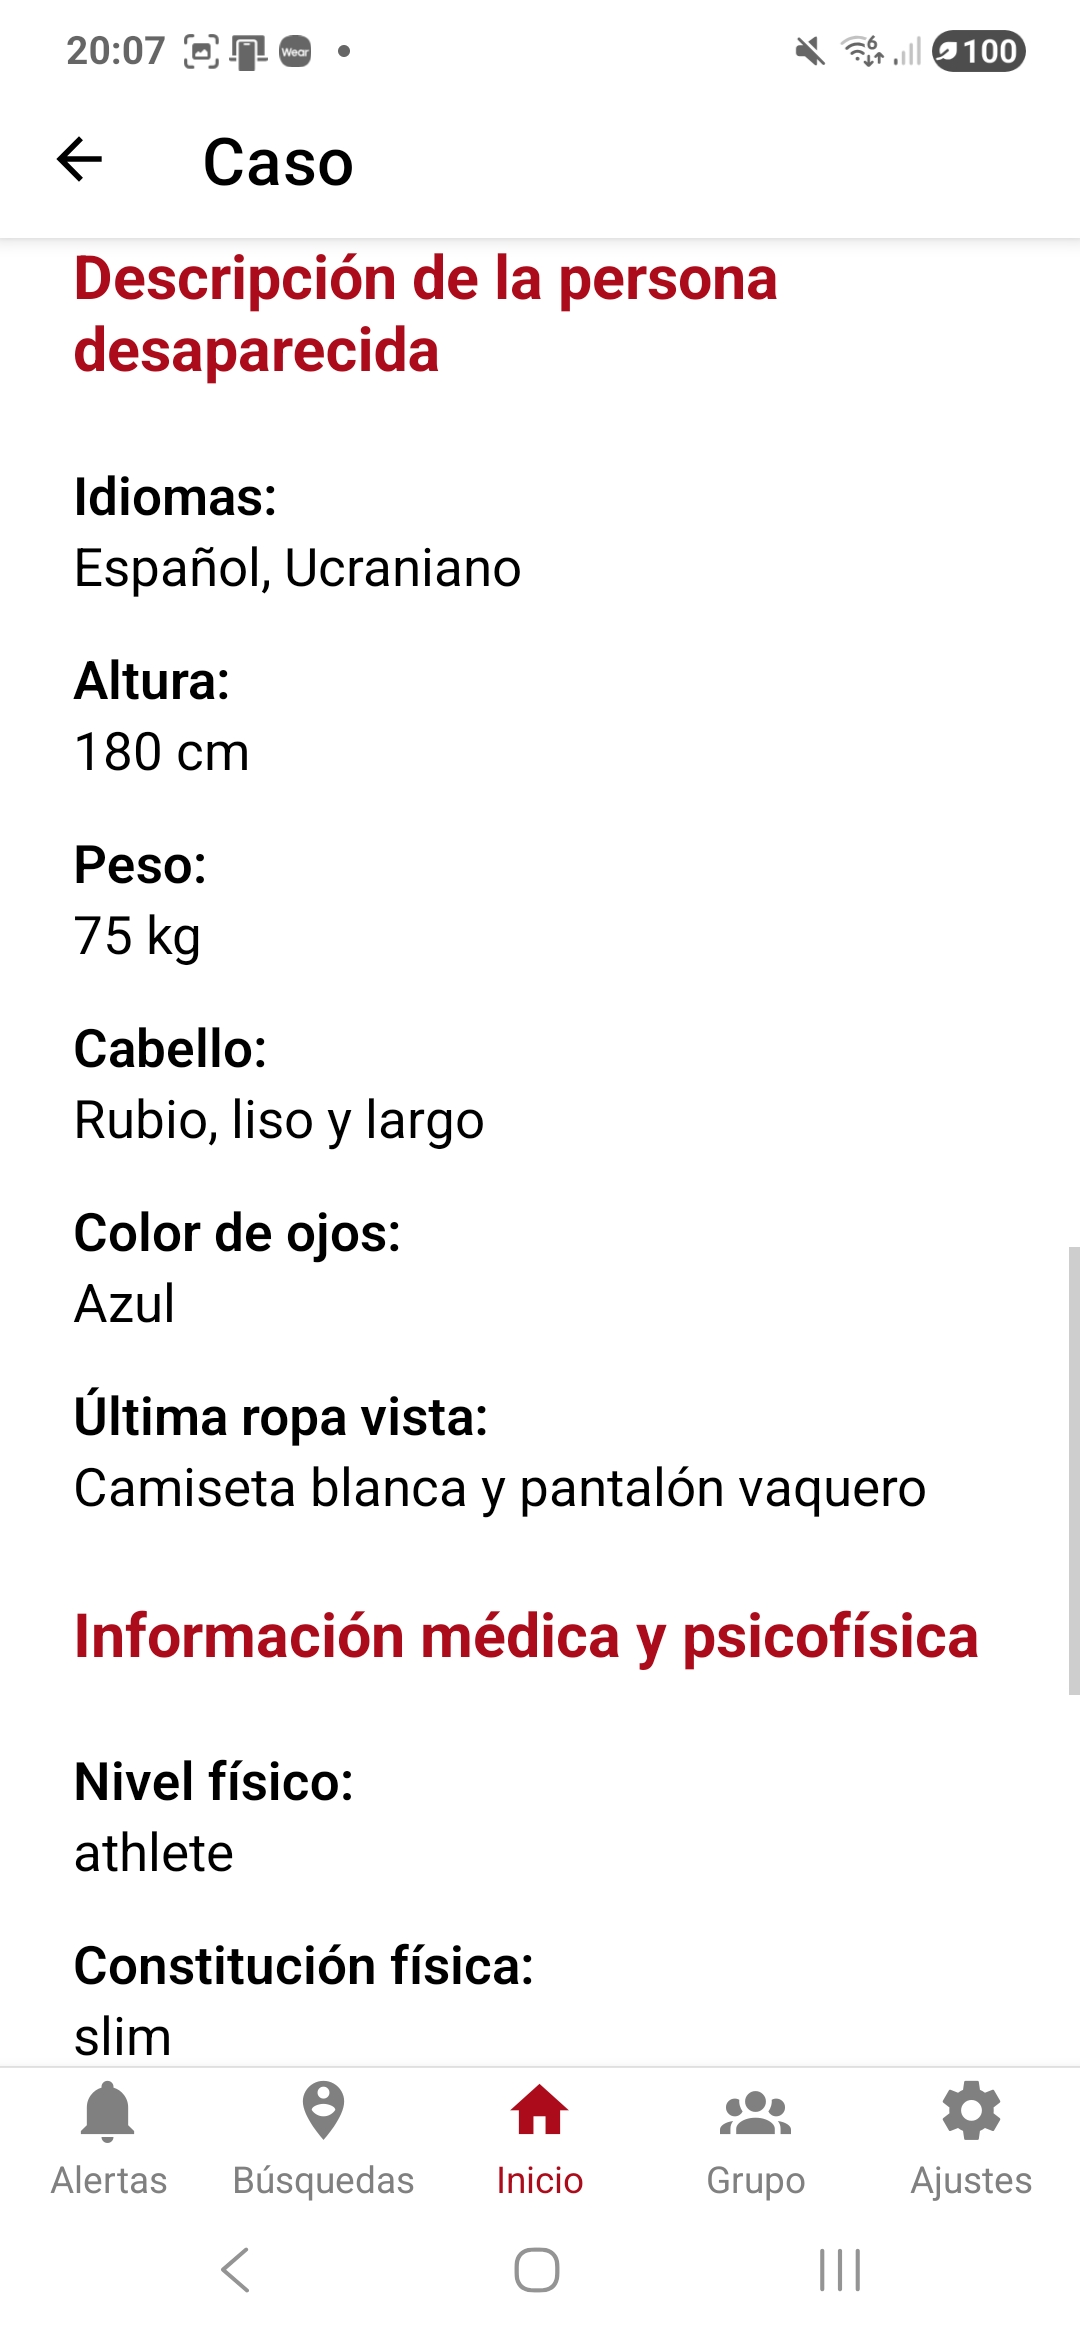
\includegraphics[width=\linewidth]{img/Resultados/Captura_AlertRes_infoGrupo.jpg}
            \caption{Información de un grupo.}
        \end{subfigure}
        \hfill
        % Tercera imagen
        \begin{subfigure}{0.33\textwidth}
            \centering
            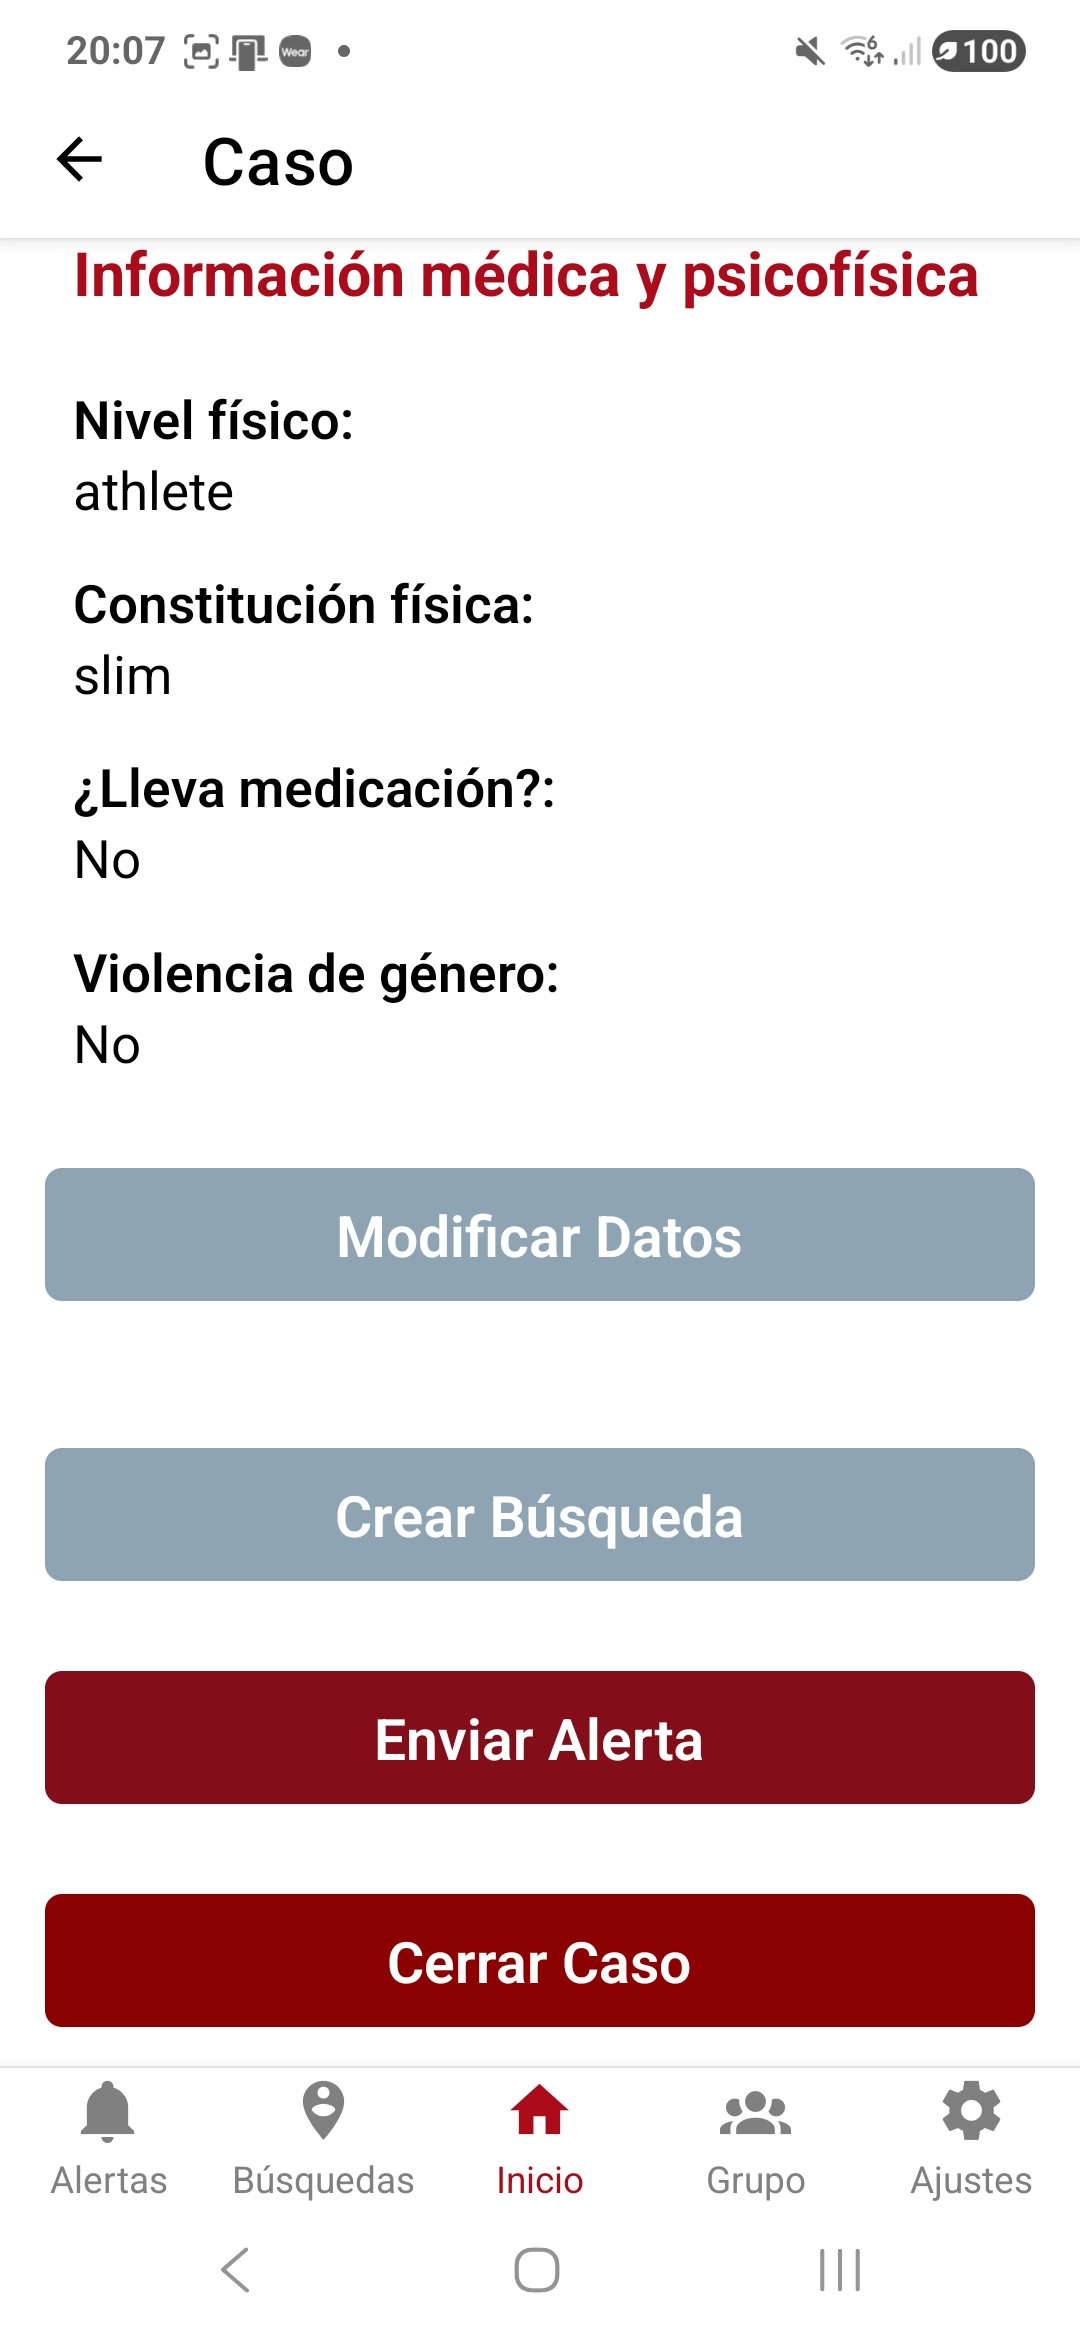
\includegraphics[width=\linewidth]{img/Resultados/Captura_AlertRes_infoGrupoModal.jpg}
            \caption{Modal de inserción de un nuevo miembro al grupo.}
            \label{app_nuevoMiembro}
        \end{subfigure}
        \caption{Pantalla de información de un grupo. \textit{Fuente propia.}}
        \label{app_infoGrupo}
    \end{figure}


\vspace{3cm}
    \subsubsection{Pantalla de cierre del caso}

    Esta pantalla se encuentra disponible una vez se presione sobre el botón de `Cerrar caso' que se encuentra en la pantalla con la información del caso, y únicamente para los usuarios con rol de `Grupo'.

    Aquí se recogen todos los campos para recuperar la información post-intervención de un incidente. Esta información se guarda en la tabla \texttt{found cases} de la base de datos y es muy importante para en el futuro poder entrenar un modelo de predicción como el que se ha propuesto previamente puesto que gracias a esta pantalla se recoge: lugar de localización, distancia y elevación que ha realizado, elevación, las horas de movilidad de la persona, el tipo de localización en el que se ha encontrado a la persona...
    
    Como en el resto de pantallas en la parte inferior se encuentra el menú principal que permite navegar al resto de pantallas a las que tiene acceso el usuario que ha iniciado sesión.

    \begin{figure}[h!]
        \centering
        % Primera imagen
        \begin{subfigure}{0.32\textwidth}
            \centering
            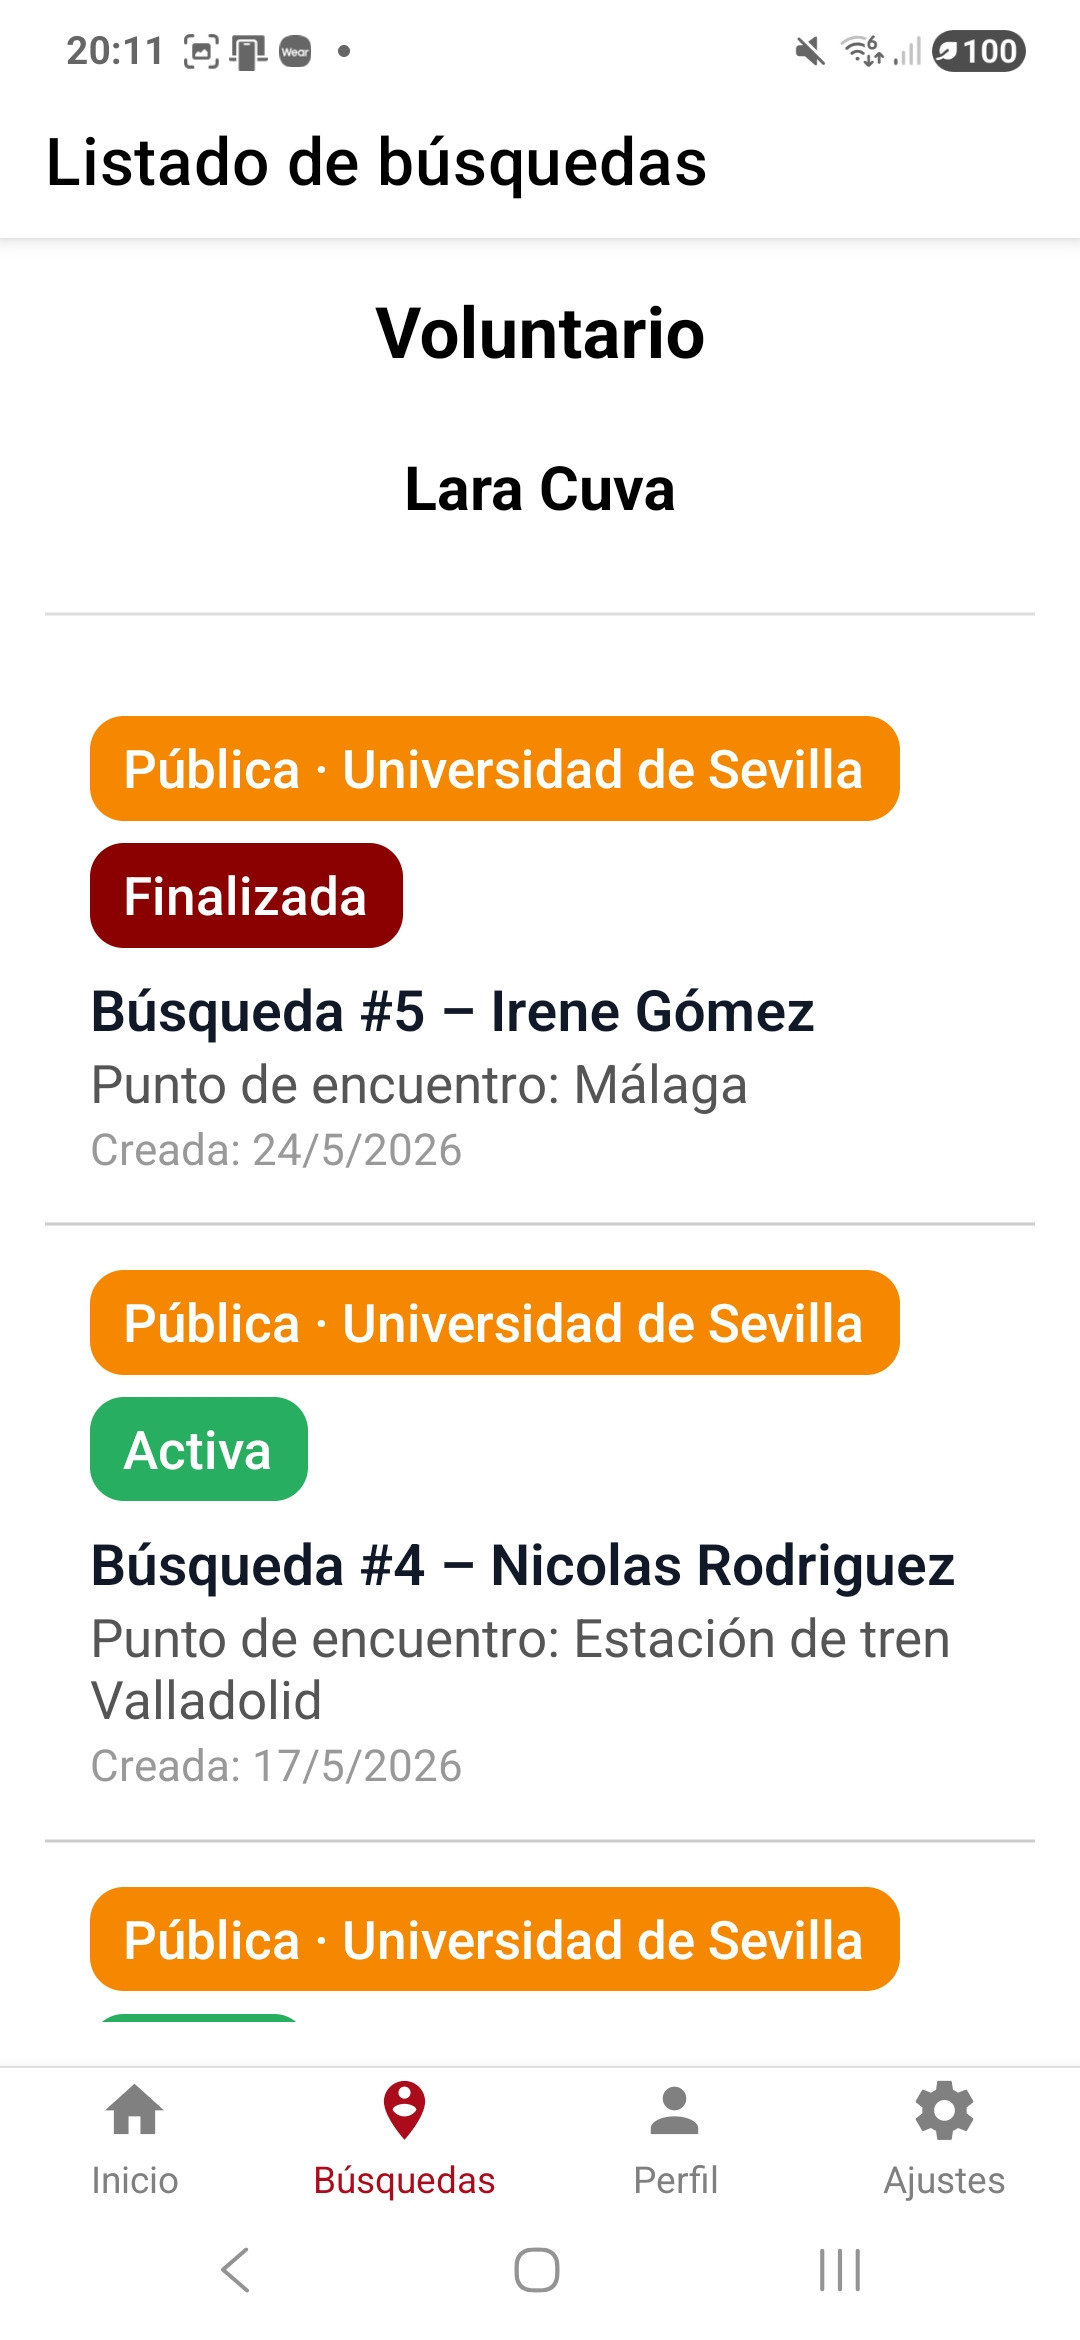
\includegraphics[width=\linewidth]{img/Resultados/Captura_AlertRes_cerrarCaso.jpg}
        \end{subfigure}
        \hfill
        % Segunda imagen
        \begin{subfigure}{0.32\textwidth}
            \centering
            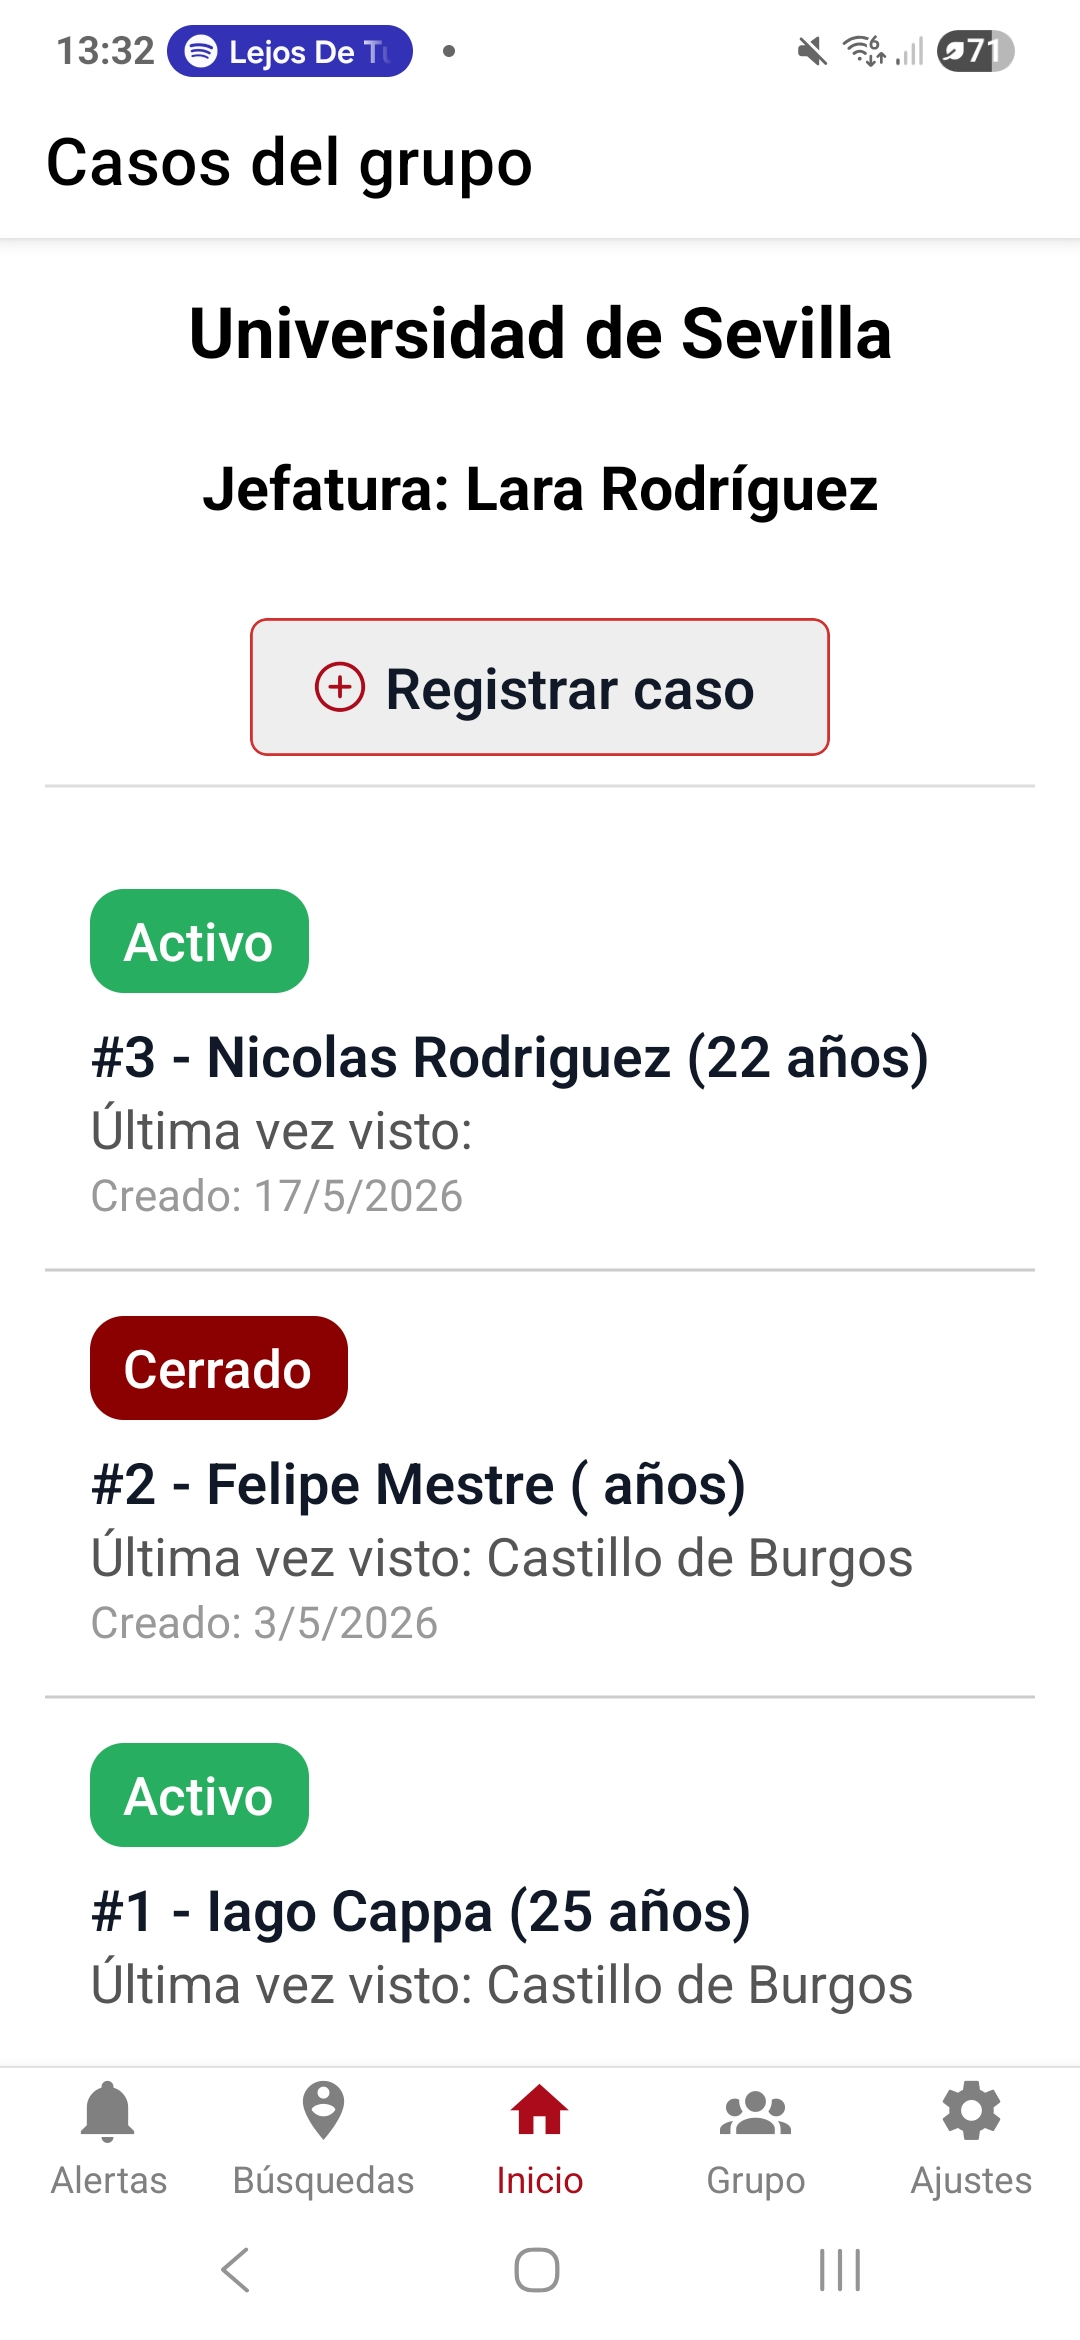
\includegraphics[width=\linewidth]{img/Resultados/Captura_AlertRes_cerrarCaso2.jpg}
        \end{subfigure}
        \hfill
        % Tercera imagen
        \begin{subfigure}{0.32\textwidth}
            \centering
            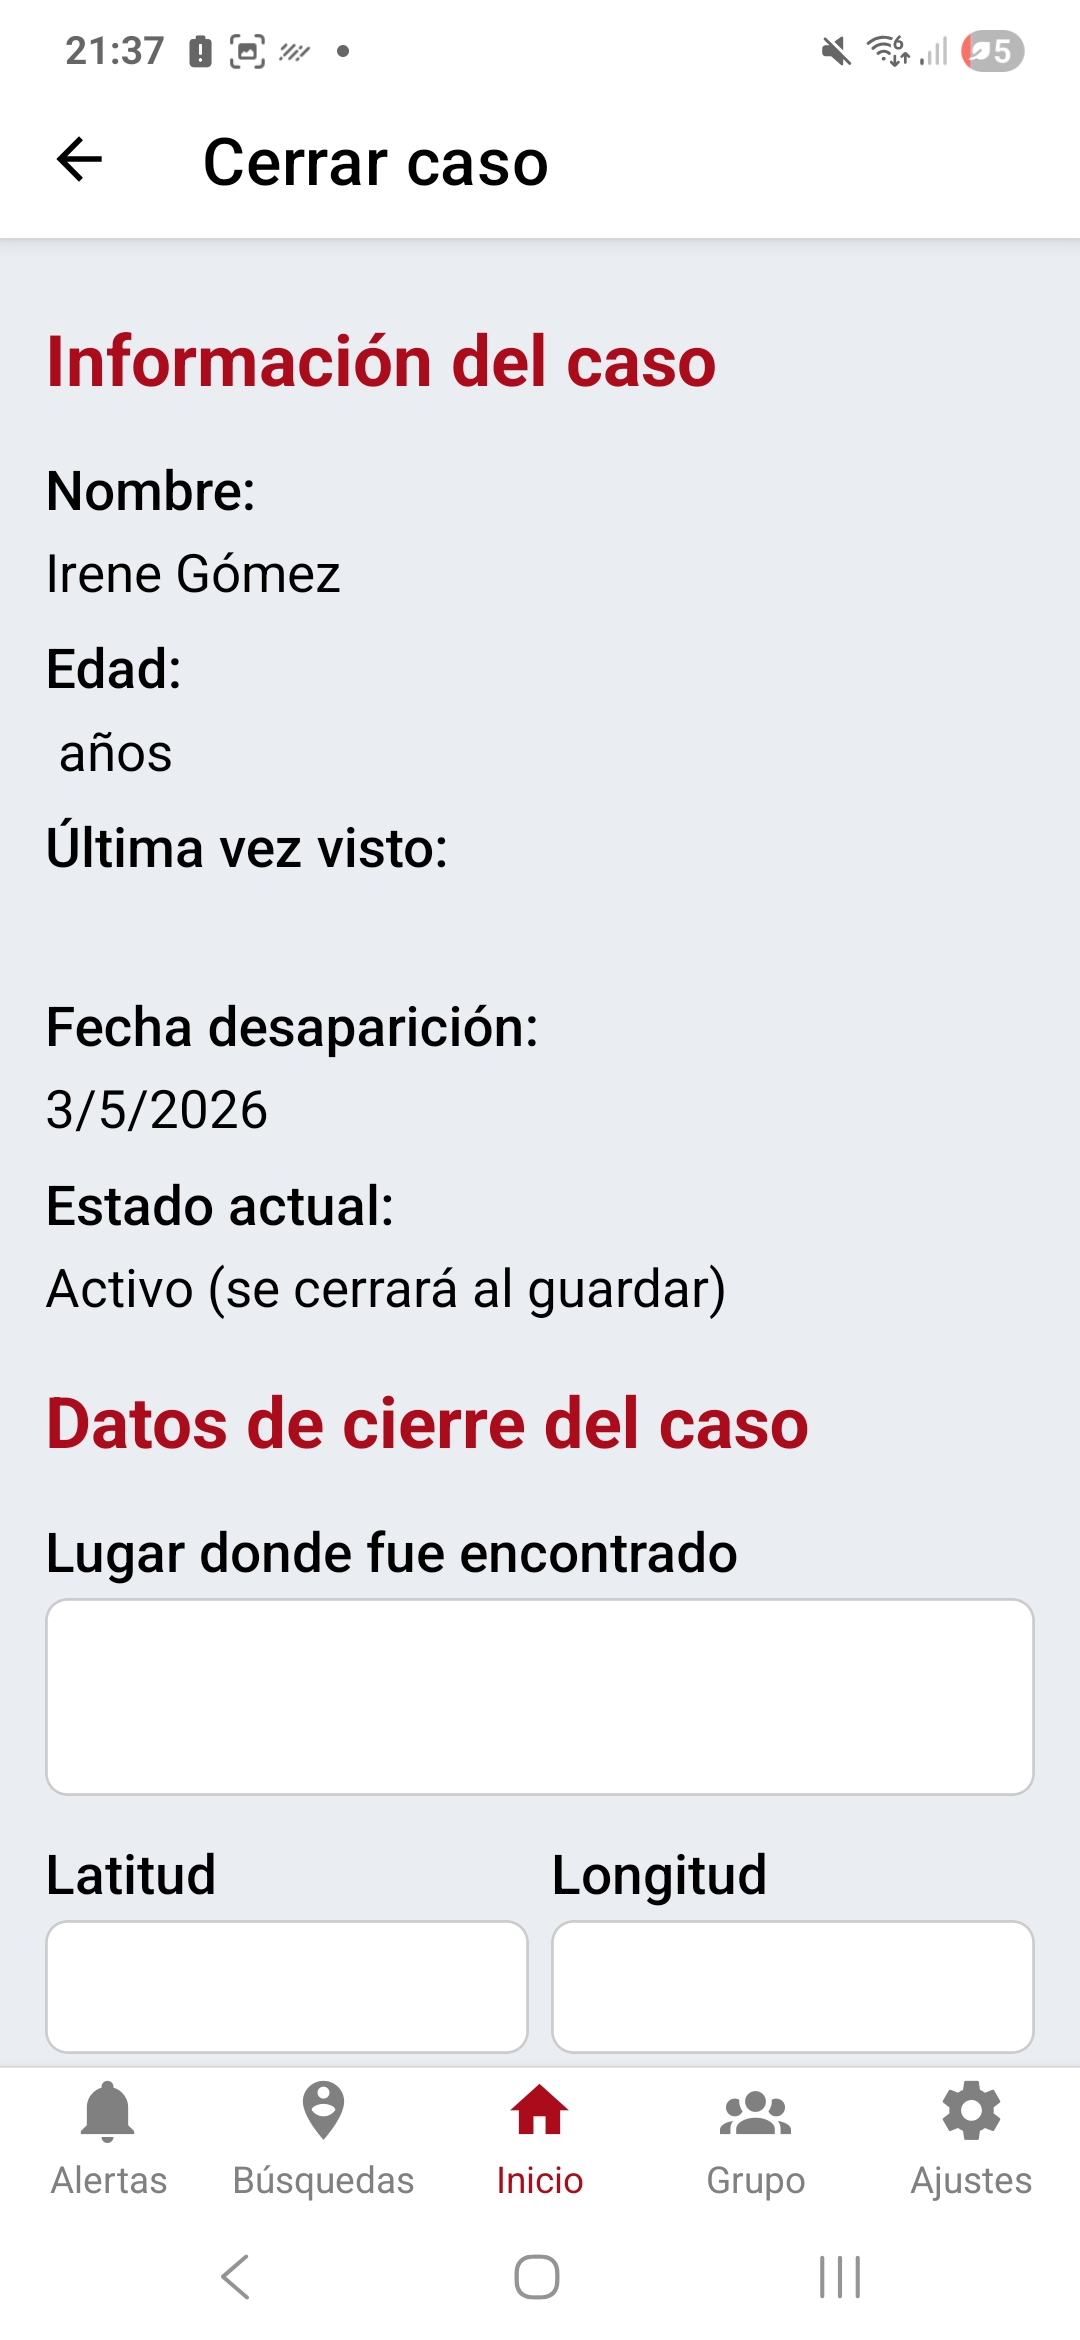
\includegraphics[width=\linewidth]{img/Resultados/Captura_AlertRes_cerrarCaso3.jpg}
        \end{subfigure}
        \caption{Pantalla de recogida de información del cierre de un caso. \textit{Fuente propia.}}
        \label{app_casoCerrado}
    \end{figure}

\vspace{3cm}
    \subsubsection{Pantalla de perfil}

    Esta pantalla es exclusivamente de los roles de `Miembros de grupo'~ y de `Voluntarios'~ y recoge la información básica del usuario. En concreto se ofrece la posibilidad de seleccionar una foto de perfil, se muestra el nombre y apellidos del usuario, un contador del número de búsquedas en las que se ha participado, sus datos de contacto, el nombre de la institución a la que pertrnece en caso de ser miembro de algún grupo y el rol que tiene como usuario.

    Además, se han incluido dos botones (actualemente sin funcionalidad real). Un primer botón que tendría em objetivo de acceder a una sere de formularios requeridos en los incidentes (confidencialidad, otros acompañantes en la búsqueda...); y, otro donde poder modificar los datos del usuario.

    Como en el resto de pantallas en la parte inferior se encuentra el menú principal que permite navegar al resto de pantallas a las que tiene acceso el usuario que ha iniciado sesión.

    \begin{figure}[h!]
        \centering
        % Primera imagen
        \begin{subfigure}{0.32\textwidth}
            \centering
            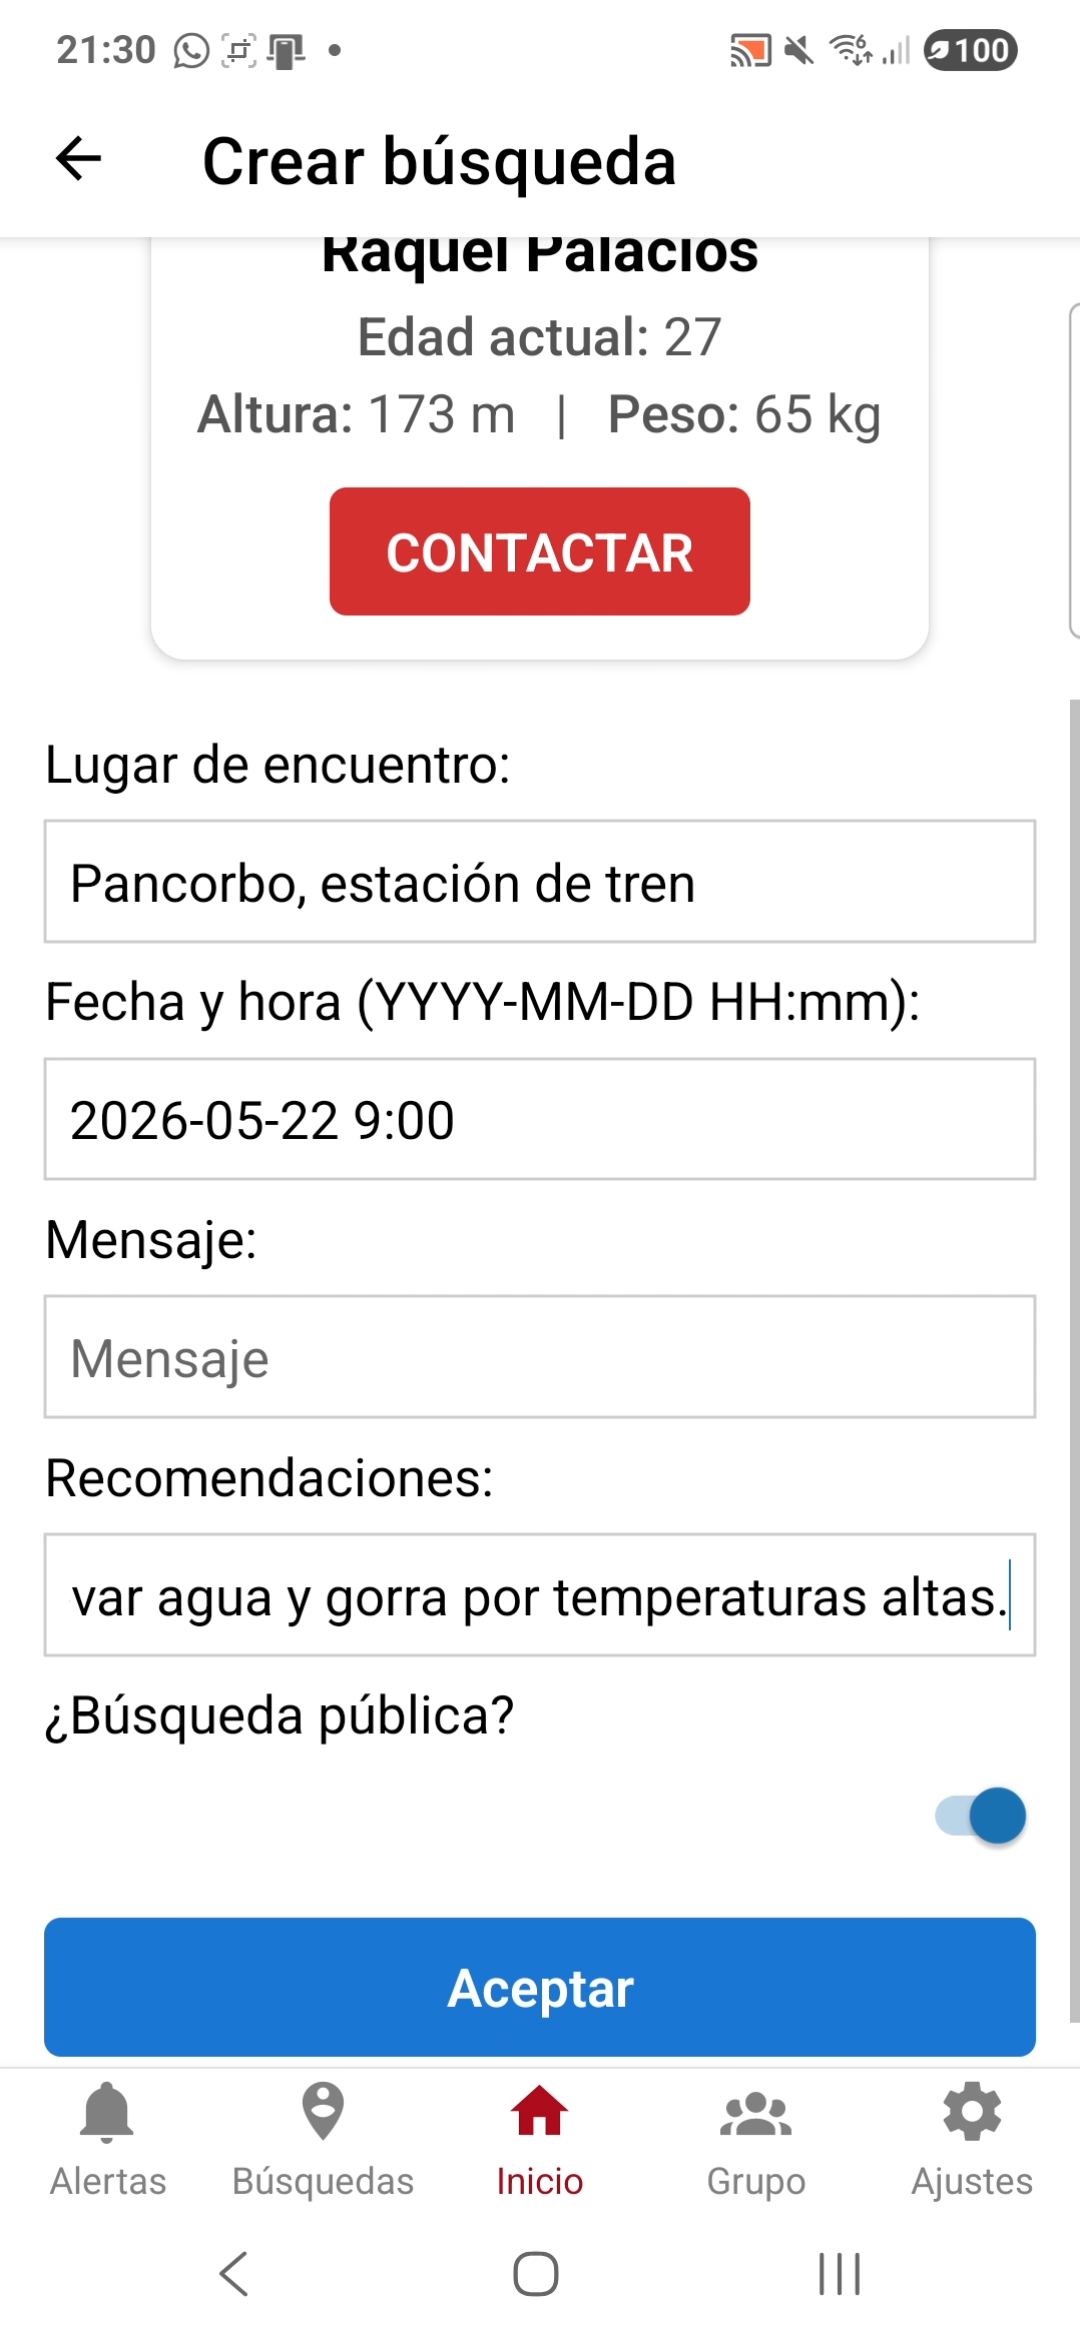
\includegraphics[width=\linewidth]{img/Resultados/Captura_AlertRes_perfilMiembro.jpg}
            \caption{Perfil de un miembro de un grupo.}
        \end{subfigure}
        \hfill
        % Segunda imagen
        \begin{subfigure}{0.32\textwidth}
            \centering
            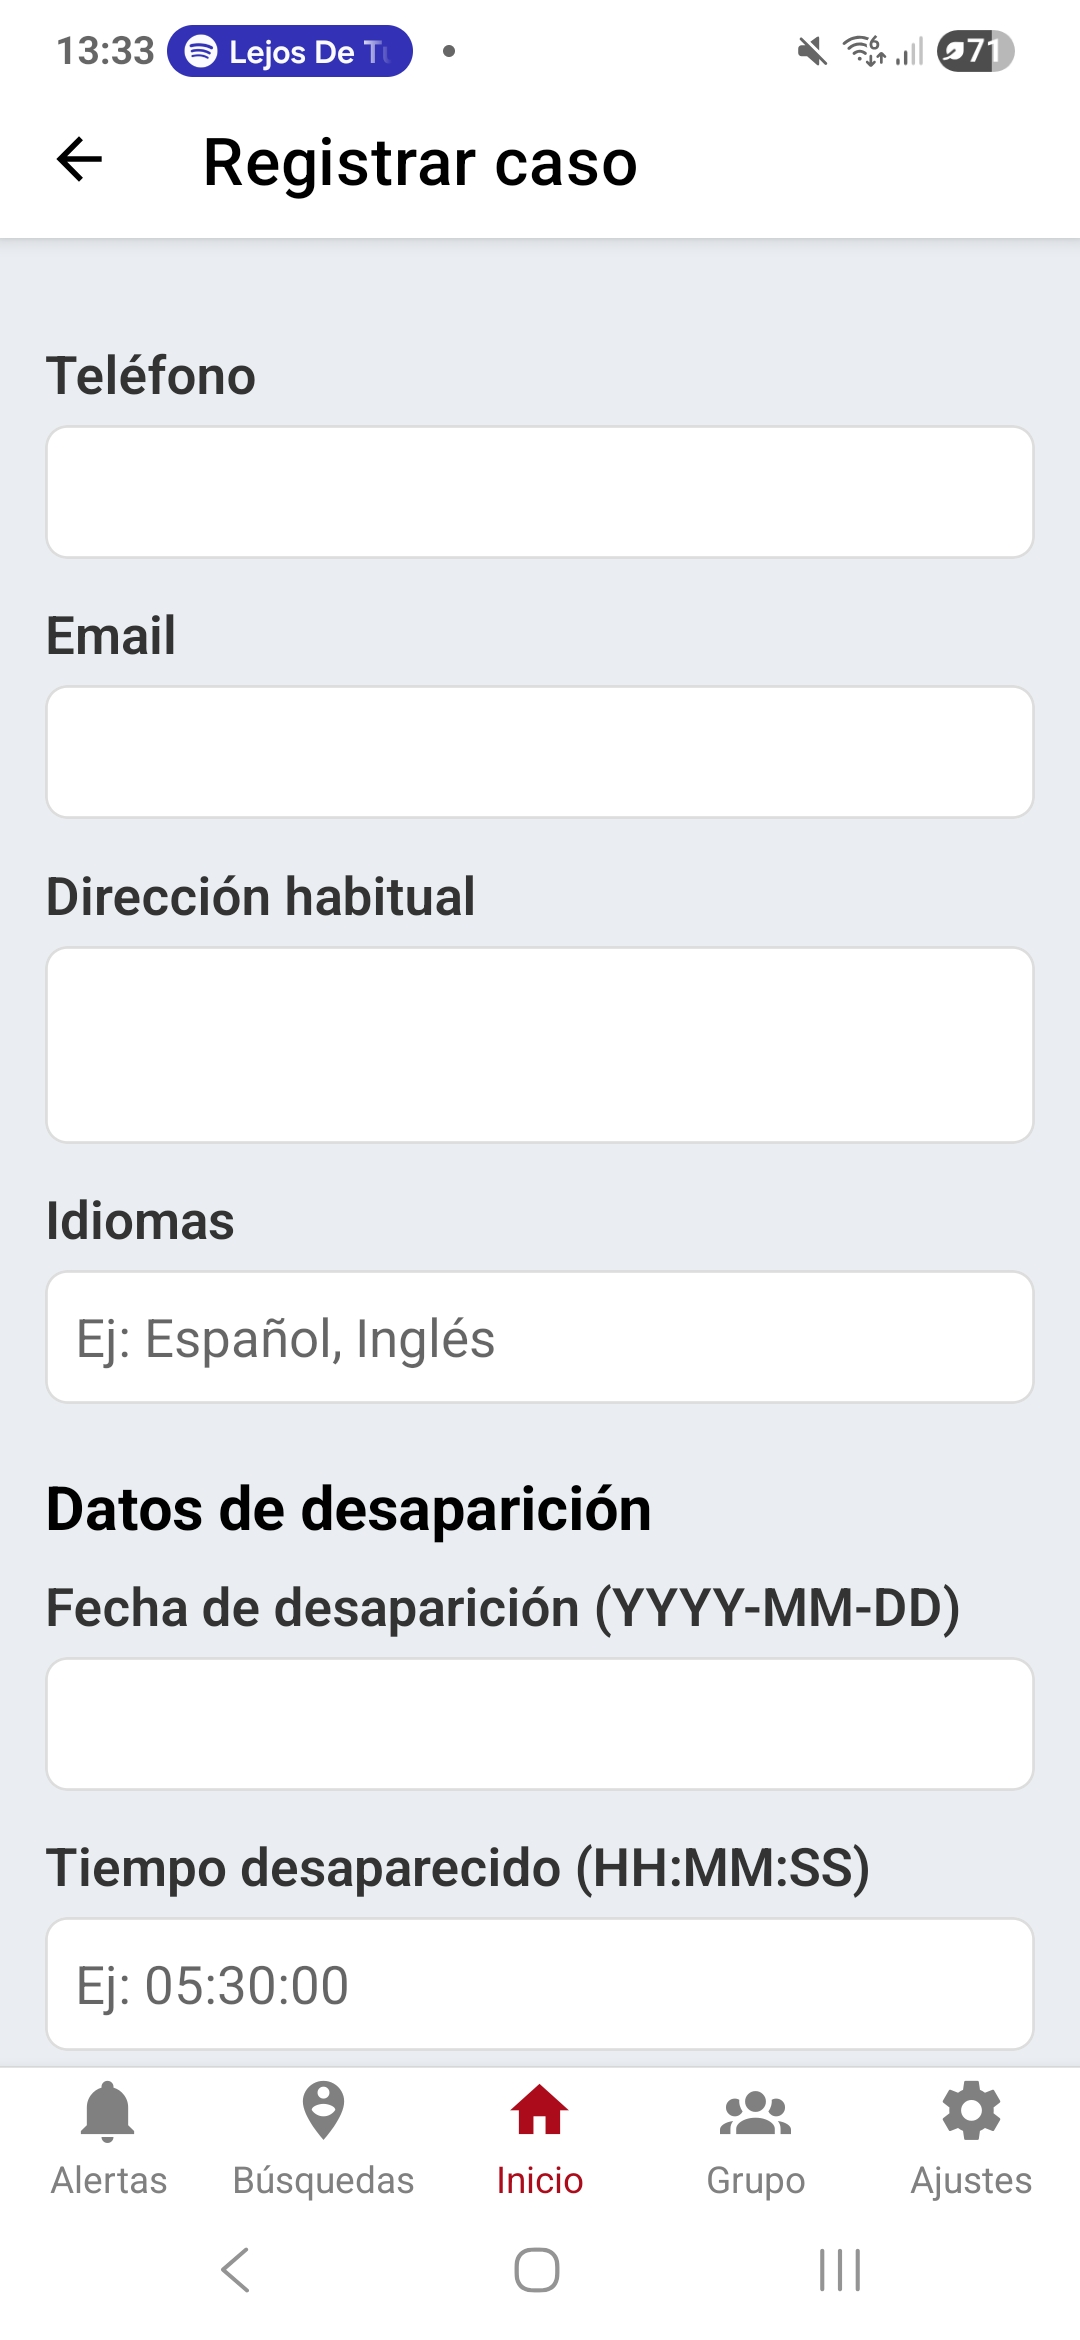
\includegraphics[width=\linewidth]{img/Resultados/Captura_AlertRes_perfilVoluntario.jpg}
            \caption{Perfil de un voluntario.}
        \end{subfigure}
        \caption{Pantalla de perfil de un usuario. \textit{Fuente propia.}}
        \label{app_perfil}
    \end{figure}

    %\figura{0.35}{img/Resultados/Web_AlertaEnviada.png}{Pantalla de perfil de un usuario. \textit{Fuente propia.}}{app_perfil}{keepaspectratio}


\vspace{3cm}
    \subsubsection{Pantalla de ajustes}

    La pantalla de ajustes de AlertRes cuenta con una serie de botones relativos a los ajustes, aunque actualmente no todos tienen funcionamiento real:
    \begin{itemize}
        \item Botón `Tutorial' que en un futuro redirigirá a un tutorial del funcionamiento de la aplicación, para apoyo a los usuarios.
        \item Switch de `Notificaciones' que en un futuro permitirá activar o desactivar las notificaciones.
        \item Botón `Cuenta' para acceder a toda la información del usuario.
        \item Botón `Privacidad' que llevará a la documentación relativa a la gestión de la privacidad por parte de AlertRes.
        \item Botón `Contacto' que muestra un modal con los datos de contacto de los encargados de la aplicación para que los usuarios puedan contactar en caso de cualquier inicidencia con la aplicación.
        \item Botón de `Cerrar sesión' que permite cerrar la cuenta y lleva automáticamente a la pantalla de inicio de sesión.
    \end{itemize}

    En la parte inferior se encuentra el menú principal que llevará al resto de pantallas a las que tiene acceso el usuario que ha iniciado sesión.

    \begin{figure}[h!]
        \centering
        % Primera imagen
        \begin{subfigure}{0.32\textwidth}
            \centering
            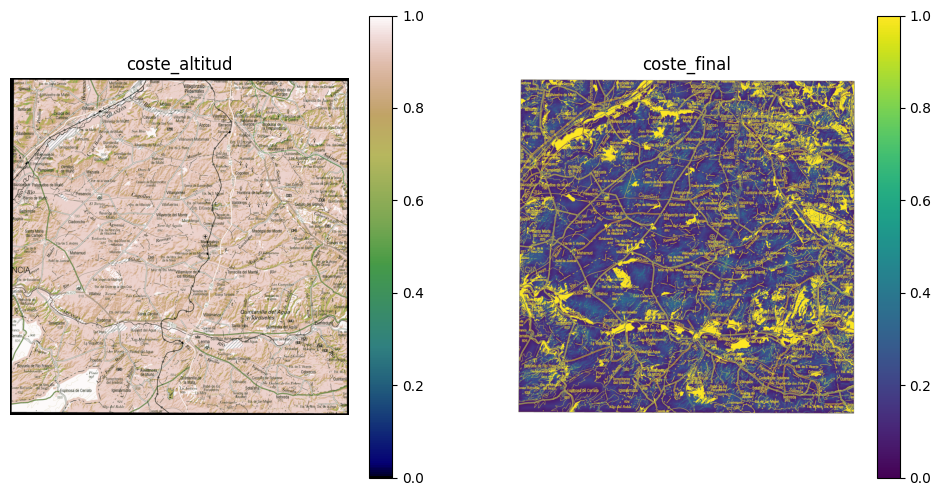
\includegraphics[width=\linewidth]{img/Resultados/Captura_AlertRes_ajustes.jpg}
        \end{subfigure}
        \hfill
        % Segunda imagen
        \begin{subfigure}{0.32\textwidth}
            \centering
            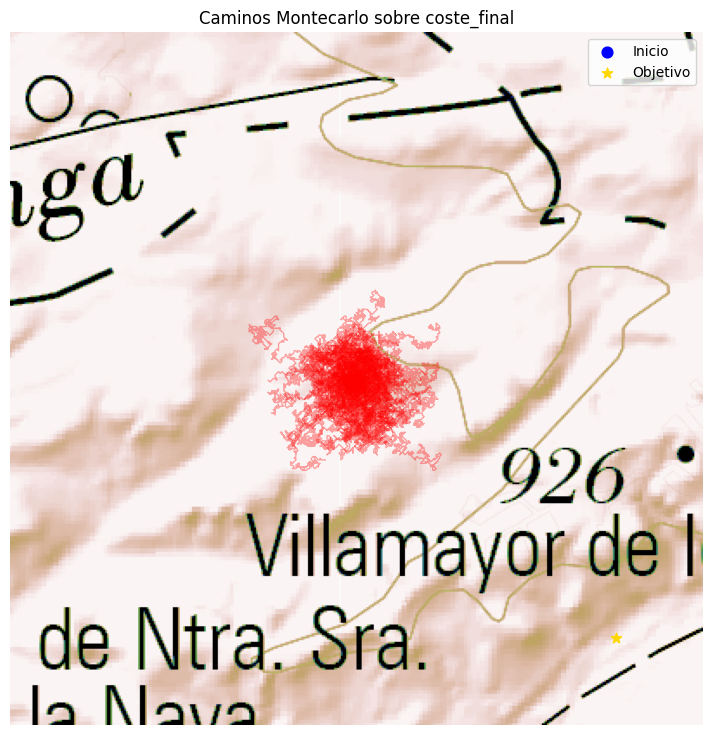
\includegraphics[width=\linewidth]{img/Resultados/Captura_AlertRes_ajustesModal.jpg}
        \end{subfigure}
        \caption{Pantalla de ajustes y modal del apartado de contacto. \textit{Fuente propia.}}
        \label{app_ajustes}
    \end{figure}



%%%%%%%%%%%%%%%%%%-------------- PRUEBAS --------------%%%%%%%%%%%%%%%%%%
    \section{Validación y pruebas}\label{pru}

   Debido a las limitaciones temporales y logísticas del proyecto, no ha sido posible llevar a cabo pruebas del prototipo. No obstante, con el objetivo de evaluar su viabilidad y adecuación a situaciones reales de búsqueda y rescate, se plantea realizar en el futuro una reunión con el grupo especializado de rescate GREM.
   
   El propósito de este encuentro será presentar el prototipo desarrollado, analizar su funcionalidad y recoger la opinión de profesionales experimentados en intervenciones reales. Asimismo, se pretende validar si el enfoque adoptado se ajusta a las necesidades operativas de este tipo de situaciones. La retroalimentación obtenida permitirá identificar posibles mejoras y ajustes necesarios.

   Como herramienta complementaria a dicha reunión, se ha diseñado un cuestionario de usabilidad dirigido a los posibles usuarios, cuyo contenido se encuentra disponible en el Anexo \ref{Anexo:CuestionarioUsabilidad}. Este cuestionario tiene como objetivo recoger información sobre aspectos clave como la facilidad de uso, la intuitividad de la interfaz, la relevancia de las funcionalidades y la adecuación general del sistema al contexto de búsqueda y rescate.
   
   Una vez realizada la reunión con el grupo GREM y aplicadas las modificaciones oportunas derivadas de sus aportaciones, se propone como siguiente fase la ejecución de simulacros controlados. Estos ensayos se llevarían a cabo tanto con miembros del propio grupo de rescate como con personas voluntarias, cuyos datos fueron recopilados durante el primer sondeo realizado al inicio del proyecto.

   En conjunto, se busca una validación progresiva del proyecto, orientado a su futura implementación en entornos reales.
%%%%%%%%%%%%%%%%%%%%%%%%%%%%%%%% INSTALACIÓN %%%%%%%%%%%%%%%%%%%%%%%%%%%%%%%%
    %\subsection{Instalación}
    

    
    %\subsection{Opiniones de usuarios}
    %He diseñado un cuestionario de usabilidad que si hubiera podido realizar pruebas se hubiese entregado a los usuarios para conocer su opinión para poder mejorar la aplicación.

%%%%%%%%%%%%%%%%%%%%%%%%%%%%%%%% PRUEBAS %%%%%%%%%%%%%%%%%%%%%%%%%%%%%%%%
    %\subsection{Pruebas de base de datos}
    %\subsection{Pruebas API(servidor)}
    %\subsection{Pruebas de la aplicación móvil}
        %\subsubsection{Android}
        %\subsubsection{iOS}